\documentclass[a4paper,UKenglish,cleveref, autoref, thm-restate]{lipics/socg-lipics-v2019}
%This is a template for producing LIPIcs articles.
%See lipics-manual.pdf for further information.
%for A4 paper format use option "a4paper", for US-letter use option "letterpaper"
%for british hyphenation rules use option "UKenglish", for american hyphenation rules use option "USenglish"
%for section-numbered lemmas etc., use "numberwithinsect"
%for enabling cleveref support, use "cleveref"
%for enabling autoref support, use "autoref"
%for anonymousing the authors (e.g. for double-blind review), add "anonymous"
%for enabling thm-restate support, use "thm-restate"

\usepackage{amsmath,amssymb,amsthm,xspace,enumitem,xcolor,tikz-cd,xspace}

\newcommand{\R}{\mathbb{R}}
\renewcommand{\S}{\mathbb{S}}
\newcommand{\T}{\mathbb{T}}
\newcommand{\W}{\mathbb{W}}
\newcommand{\X}{\mathbb{X}}
\newcommand{\Y}{\mathbb{Y}}
\newcommand{\Z}{\mathbb{Z}}

\renewcommand{\AA}{\mathbb{A}}
\newcommand{\BB}{\mathbb{B}}
\newcommand{\FF}{\mathbb{F}}
\newcommand{\LL}{\mathbb{L}}
\newcommand{\UU}{\mathbb{U}}
\newcommand{\VV}{\mathbb{V}}

\newcommand{\A}{\mathcal{A}}
\newcommand{\E}{\mathcal{E}}
\newcommand{\F}{\mathcal{F}}
\newcommand{\I}{{\mathcal{I}}}
\newcommand{\J}{\mathcal{J}}
\newcommand{\N}{\mathcal{N}}
\newcommand{\U}{\mathcal{U}}
\newcommand{\V}{\mathcal{V}}

\newcommand{\e}{\varepsilon}
\newcommand{\im}{\mathbf{im}\xspace}
\renewcommand{\ker}{\mathbf{ker}\xspace}
\newcommand{\rk}{\mathbf{rk\xspace}}
\renewcommand{\dim}{\mathbf{dim}\xspace}
\newcommand{\rest}{\mathord{\mid}}

\newcommand{\cech}{\check{\mathcal{C}}}
\newcommand{\rips}{\mathcal{R}}
\newcommand{\ball}{\mathbf{ball}}
\newcommand{\dist}{\mathbf{d}}

\newcommand{\cl}{\mathbf{cl\xspace}}
\newcommand{\intr}{\mathbf{int\xspace}}

\newcommand{\Hom}{\mathrm{Hom}}
\renewcommand{\hom}{\mathrm{H}}

\newcommand{\subi}[2]{_{\scriptscriptstyle #2\mid #1}}

\newcommand{\D}[2]{\mathcal{D}\subi{#1}{#2}}
\newcommand{\DD}[1]{\mathbb{D}_{#1}}

\renewcommand{\P}[3]{\mathcal{P}\subi{#1}{#3}^{#2}}
\newcommand{\CP}[3]{\cech\P{#1}{#2}{#3}}
\newcommand{\RP}[3]{\rips\P{#1}{#2}{#3}}

\newcommand{\PP}[2]{\mathbb{P}_{#1}^{#2}}
\newcommand{\CPP}[2]{\cech\PP{#1}{#2}}
\newcommand{\RPP}[2]{\rips\PP{#1}{#2}}

\newcommand{\ext}[1]{\E\xspace #1}

\newcommand{\fullversion}{Appendix} %{full version of this paper}

\bibliographystyle{plainurl}

\title{From Coverage Testing to Topological Scalar Field Analysis}

% Please enter author specific funding statements as fifth argument of the \author macro.
\author{Kirk P. Gardner}{North Carolina State University, United States}{kpgardn2@ncsu.edu}{https://orcid.org/0000-0001-5306-2174}{}
\author{Donald R. Sheehy}{North Carolina State University, United States}{don.r.sheehy@gmail.com}{https://orcid.org/0000-0002-9177-2713}{}

\authorrunning{K.\,P. Gardner and D.\,R. Sheehy}

\Copyright{Kirk P. Gardner and Donald R. Sheehy}

\begin{CCSXML}
  <ccs2012>
    <concept>
      <concept_id>10002950.10003741.10003742.10003744</concept_id>
      <concept_desc>Mathematics of computing~Algebraic topology</concept_desc>
      <concept_significance>500</concept_significance>
    </concept>
    <concept>
      <concept_id>10003752.10010061.10010063</concept_id>
      <concept_desc>Theory of computation~Computational geometry</concept_desc>
      <concept_significance>300</concept_significance>
    </concept>
  </ccs2012>
\end{CCSXML}

\ccsdesc[500]{Mathematics of computing~Algebraic topology}
\ccsdesc[300]{Theory of computation~Computational geometry}


\keywords{topology, homology, coverage, scalar fields, persistent homology, relative homology}

% \category{} %optional, e.g. invited paper

% \relatedversion{} %optional, e.g. full version hosted on arXiv, HAL, or other respository/website
%\relatedversion{A full version of the paper is available at \url{...}.}

% \supplement{}%optional, e.g. related research data, source code, ... hosted on a repository like zenodo, figshare, GitHub, ...

 %optional, to capture a funding statement, which applies to all authors.
\funding{This research was supported by the NSF under grants CCF-1525978 and CCF-1652218.}

% \acknowledgements{I want to thank \dots}%optional

%\nolinenumbers %uncomment to disable line numbering

%\hideLIPIcs  %uncomment to remove references to LIPIcs series (logo, DOI, ...), e.g. when preparing a pre-final version to be uploaded to arXiv or another public repository

%Editor-only macros:: begin (do not touch as author)%%%%%%%%%%%%%%%%%%%%%%%%%%%%%%%%%%
\EventEditors{John Q. Open and Joan R. Access}
\EventNoEds{2}
\EventLongTitle{42nd Conference on Very Important Topics (CVIT 2016)}
\EventShortTitle{CVIT 2016}
\EventAcronym{CVIT}
\EventYear{2016}
\EventDate{December 24--27, 2016}
\EventLocation{Little Whinging, United Kingdom}
\EventLogo{}
\SeriesVolume{42}
\ArticleNo{23}
%%%%%%%%%%%%%%%%%%%%%%%%%%%%%%%%%%%%%%%%%%%%%%%%%%%%%%

\begin{document}

\maketitle

% !TeX root = ../main.tex

\begin{abstract}
  The topological coverage criterion (TCC) can be used to test whether an underlying space is sufficiently well covered by a given data set.
  Given a sufficiently dense sample, topological scalar field analysis (SFA) can give a summary of the shape of a real-valued function on its domain.
  The goal of this paper is to put these theories together so that one can test coverage with the TCC while computing a summary with SFA.
  The challenge is that the TCC requires a well-defined boundary that is not generally available in the setting of SFA.
  To overcome this, we show how the scalar field itself can be used to define a boundary that can be used to confirm coverage.
  % This requires a generalization of the TCC proof and resolves one of the major barriers to wider use of the TCC.
  This requires an interpretation of the TCC that resolves one of the major barriers to wider use.
  % It also extends SFA methods to a wider class of spaces.
  It also extends SFA methods to the setting in which coverage is only confirmed in a subset of the domain. %a space surrounded by a sub-levelset.
  % We show how the intersection of these two theories can be used to approximate the persistent homology relative to a static sublevel set.
  % We then discuss how this persistent relative homology relates to that of the scalar field as a whole.
\end{abstract}


\section{Introduction}\label{sec:introduction}
% !TeX root = ../main.tex

In the topological analysis of scalar fields (SFA), one computes a topological summary capturing qualitative and quantitative shape information from a set of points endowed with a metric and a real-valued function.
That is, we have points with distances and a real number assigned to each point.
More generally, it usually suffices to have a neighborhood graph on the points identifying the pairs of points that close.
The topological computation often takes the form of persistent homology and integrates the local information from the function into global information about the behavior of the function on the entire space.
In prior work, Chazal et al.~\cite{XXX} showed that for sufficiently dense samples on sufficiently smooth spaces, the persistence diagram can be computed with some guarantees.
In followup work, Buchet et al.~\cite{XXX} extended this result to show how to work with noisy inputs.
A fundamental assumption required to have strong guarantees on the output of these methods is that the underlying space be sufficiently well-sampled.
In this paper, we show how to combine scalar fields analysis with the theory of topological coverage testing to simultaneously compute the persistence diagram and also to test that the underlying space is sufficiently well-sampled.

Initiated by De Silva and Ghrist~\cite{XXX,XXX,XXX}, the theory of homological sensor networks addresses the problem of testing coverage of a bounded domain by a collection of sensors without localization.
The main result is the topological coverage criterion, which, in its most general form, states that under reasonable geometric assumptions, the $d$-dimensional homology of a pair of simplicial complex built on the neighborhood graph will be nontrivial if and only if there is sufficient coverage (see Section~\ref{sec:tcc} for the precise statements).
This relative persistent homology test is called the Topological Coverage Criterion (TCC).
Cavanna et al.~\ref{cavanna2017when} generalized the TCC to allow for more general spaces and robust coverage guarantees.

Superficially, the methods of SFA and TCC are very similar.
Both construct similar complexes and compute the persistent homology of the homological image of a complex on one scale into that of a larger scale.
They even overlap on some common techniques in their analysis including the use of the Nerve theorem and the Rips-\v{C}ech interleaving.
However, they differ in some fundamental way that makes it difficult to combine them into a single technique.
The main difference is that the TCC requires a clearly defined boundary.
Not only must the underlying space be a bounded subset of $\R^d$, the data must also be labeled to indicate which input points are close to the boundary.
This requirement is perhaps the main reason why the TCC can so rarely be applied in practice.

Moreover, as a necessary but not sufficient condition for coverage there is room to question what can go wrong in the case of false positives.
In fact, the efficacy of the condition relies on having enough sensors close enough to approximate the boundary in homology.
This leads us to believe the condition checks for something more specific than coverage alone.
Specifically, that we have a sample as well as a subsample that reflect the topology of the space and its boundary as a pair.


\section{Summary}\label{sec:summary}
% !TeX root = ../main.tex

Let $\X$ denote an orientable $d$-manifold and $D\subset\X$ a compact subspace.
For a $c$-Lipschitz functon $f : D\to \R$ and $\alpha\in\R$ let $B_\alpha := f^{-1}((-\infty,\alpha])$ denote the $\alpha$-sublevel set of $f$.
Our sample will be denoted $P$, and the subset of points sampling $B_\alpha$ will be denoted $Q_\alpha := P\cap B_\alpha$.
For $\e > 0$ let $P^\e$ denote the union of open metric balls centered at points in $P$.
For ease of exposition let
\[ D\subi{z}{\alpha} := B_\alpha\cup B_z \]
denote the \emph{$z$-truncated} sublevel sets of $f$ and % of the restricted function $f\rest_{D\setminus B_w}$ for all $\alpha,w\in\R$.
\[ P\subi{z}{\alpha} := Q_\alpha\cup Q_z\]
for all $z,\alpha\in\R$.

We will select a sublevel set $B_\omega$ of $f$ that \emph{surrounds} $D$ to serve as our boundary.
Given a sample of $f$ at a finite number of points $P$ in $D$ we would like to confirm $P^\delta$ not only covers the interior $D\setminus B_\omega$, but also that $Q^\delta$ surrounds $P^\delta$ for some $Q\subset P$.
That is, we would like to verify that a pair $(P^\delta, Q^\delta)$ is representative of the pair $(D,B_\omega)$ in homology.
Our goal is to use this fact to approximate the persistence of $f$ relative to $B_\omega$.

Our approximation will be by a nested pair of (Vietoris-)Rips complexes, denoted $\rips^\e(P, Q) = (\rips^\e(P), \rips^\e(Q))$ for $\e > 0$.
Under mild regularity assumptions it can be shown that
\[ \rk~\hom_d(\rips^\delta(P, Q_{\omega - 2c\delta})\hookrightarrow \rips^{2\delta}(P, Q_{\omega+c\delta}))\geq \dim~\hom_0(\rips^\delta(P\setminus Q_{\omega-2c\delta}))\]
implies $D\setminus B_\omega\subseteq P^\delta$ and $Q_{\omega-2c\delta}^\delta$ surrounds $P^\delta$ in $D$.
Proof of this fact generalizes that of the TCC to boundaries defined in terms of a function $f$, eliminating unnatural assumptions made in previous work.
Not only are our subsamples $Q_{\omega-2c\delta}$ and $Q_{\omega+c\delta}$ defined by their function values, but our regularity assumptions can now be stated directly in terms of the persistent homology of $f$.

Given a sample $P$ that satisfies the TCC we can approximate the persistent homology of $f$ as follows.
The nested pair of Rips complexes used to confirm coverage can be extended to a filtration
\[ \{\rips^{2\delta}(P\subi{\omega-2c\delta}{\alpha}, Q_{\omega-2c\delta})\hookrightarrow \rips^{4\delta}(P\subi{\omega+c\delta}{\alpha}, Q_{\omega+c\delta})\}_{\alpha\in\R}\]
that can be used to approximate the persistent homology of $\{(D\subi{\omega}{\alpha}, B_\omega)\}_{\alpha\in\R}$.
% Indeed, we could use existing methods to approximate the persistent homology of $f$ \emph{restricted} to the subspace $D\setminus B_\omega$ that we cover.
% However, the question of what this would approximate is important to consider.
% {\color{red} Restricting the domain of the function can not only introduce noise close to the boundary, \textbf{but also perturb global structure in our signature.}\footnote{\color{red} close.}}
% As an alternative, we approximate the persistence of $f$ \emph{relative} to the sublevel set $B_\omega$.
The use of images of relative persistence modules is not only to eliminate noise at the boundary, but also to \emph{truncate} the persistence of $f$ in a way that isolates global structure.

\paragraph*{Outline}

We will begin with our statement of the TCC in Section~\ref{sec:tcc}.
A Part of the proof of the TCC will be generalized to properties of \emph{surrounding pairs}, simplifying our reformulation of the TCC in Theorem~\ref{thm:algo_tcc}.
Section~\ref{sec:middle} introduces extensions of surrounding pairs, as well as partial interleavings of image modules.
These are the main technical results used to show that a positive result from the TCC verifies that a surrounding pair of samples can be used to approximate the persistence of a function relative to a sublevel set in Theorem~\ref{thm:interleaving_main_2}.
In Section~\ref{sec:truncations} we provide an interpretation of this relative persistence as a truncation of the full diagram (i.e., the persistence of $f$ on all of $D$) that is motivated by examples from a proof-of-concept implementation in Section~\ref{sec:experiments}.


\section{The Topological Coverage Criterion (TCC)}\label{sec:tcc}
% !TeX root = ../main.tex

A positive result from the TCC requires that we have a subset of our cover to serve as the boundary.
That is, the the condition not only checks that we have coverage, but also that we have a pair of spaces that reflects the pair $(D, B)$ topologically.
We call such a pair a \emph{surrounding pair} defined in terms of separating sets.
It has been shown that the TCC can be stated in terms of these surrounding pairs and that assumptions can be made directly in terms of their persistent homology~\cite{cavanna2017when}.
This allows allows us enough flexibility to define our surrounding set as a sublevel of a $c$-Lipschitz function $f$ and state our assumptions in terms of its persistent homology.

\begin{definition}[Surrounding Pair]
  Let $X$ be a topological space and $(D,B)$ a pair in $X$.
  The set $B$ \textbf{surrounds $D$ in $X$} if $B$ separates $X$ with the pair $(D\setminus B, X\setminus D)$.
  We will refer to such a pair as a \textbf{surrounding pair in $X$}.
\end{definition}

For a surrounding pair $(D,B)$ in $X$  the complement $\overline{B} = X\setminus B$ is the union of disconnected sets $X\setminus D$ and $D\setminus B$.
Therefore, $\hom_k(\overline{B}) \cong \hom_k(\overline{D})\oplus \hom_k(D\setminus B)$ thus $\hom_k(\overline{B},\overline{D})\cong \hom_k(D\setminus B)$ for all $k$.
The following lemma generalizes the proof of the TCC as a property of surrounding sets.
We will then combine these results on the homology of surrounding pairs with information about both $X$ as a metric space and our function.

\begin{lemma}\label{lem:coverage}
  Let $(D, B)$ be a surrounding pair in $X$ and $U\subseteq D$, $V\subseteq U\cap B$ be subsets.
  Let $\ell: \hom_0(X\setminus B, X\setminus D)\to \hom_0(X\setminus V, X\setminus U)$ be induced by inclusion.

  If $\ell$ is injective then $D\setminus B\subseteq U$ and $V$ surrounds $U$ in $D$.
\end{lemma}

Let $(\X,\dist)$ be a metric space and $D\subseteq \X$ be a compact subspace.
For a $c$-Lipschitz function $f : D\to \R$ we introduce a constant $\omega$ as a threshold that defines our ``boundary'' as a sublevel set $B_\omega$ of the function $f$.
Let $P$ be a finite subset of $D$ and $\zeta\geq\delta > 0 $ be constants such that $P^\delta\subseteq \intr_\X(D)$.
Here, $\delta$ will serve as our communication radius where $\zeta$ is reserved for use in Section~\ref{sec:middle}.
  \footnote{We will set $\zeta = 2\delta$ in the proof of our interleaving with Rips complexes but the TCC holds for all $\zeta\geq\delta$.}

\begin{lemma}\label{lem:psurj}
  Let $i : \hom_0(\overline{Q_{\omega+c\delta}^\delta}, \overline{P^\delta})\to \hom_0(\overline{Q_{\omega-c\zeta}^\delta}, \overline{P^\delta})$.

  If $B_\omega$ surrounds $D$ in $\X$ then $\dim~\hom_0(\overline{B_\omega}, \overline{D})\geq \rk~i$.
\end{lemma}
\begin{proof}
  Choose a basis for $\im~i$ such that each basis element is represented by a point in $P^\delta\setminus Q_{\omega+c\delta}^\delta$.
  Let $x\in P^\delta\setminus Q_{\omega+c\delta}^\delta$ be such that $i[x]$ is non-trivial.
  So there exits some $p\in P$ such that $\dist(p, x) < \delta$ and $p\notin Q_{\omega+c\delta}$, otherwise $x\in Q_{\omega+c\delta}^\delta$.
  Therefore, because $f$ is $c$-Lipschitz,
  \[ f(x)\geq f(p) - c\dist(x, p) > \omega.\]

  So $x\in\overline{B_\omega}$ and, because $x\in P^\delta\subseteq D$ it follows that $x\in D\setminus B_\omega$.
  Because $i$ and $\ell : \hom_0(\overline{B_\omega}, \overline{D})\to \hom_0(\overline{Q_{\omega-c\zeta}^\delta}, \overline{P^\delta})$ are induced by inclusion $\ell[x] = i[x]$ is non-trivial in $\hom_0(\overline{Q_{\omega-c\zeta}^\delta}, \overline{P^\delta})$.
  That is, every element of $\im~i$ has a preimage in $\hom_0(\overline{B_\omega}, \overline{D})$, so we may conclude that $\dim~\hom_0(\overline{B_\omega}, \overline{D})\geq \rk~i$.
\end{proof}

While there is a surjective map from $\hom_0(\overline{B_\omega}, \overline{D})$ to $\im~i$ this map is not necessarily induced by inclusion.
We will therefore introduce a larger space $B_{\omega+c(\delta+\zeta)}$ that contains $Q_{\omega+c\delta}^\delta$ in order to provide a criteria for the injectivity of $\ell : \hom_0(\overline{B_\omega}, \overline{D})\to\hom_0(\overline{Q_{\omega-c\zeta}^\delta}, \overline{P^\delta})$ in terms of $\rk~i$.
We have the following commutative diagrams of inclusion maps and maps induced by inclusion between complements in $\X$.

\begin{equation}\label{dgm:1}
\begin{tikzcd}
  (P^\delta, Q_{\omega-c\zeta}^\delta) \arrow[hookrightarrow]{r}\arrow[hookrightarrow]{d} &
  (P^\delta, Q_{\omega+c\delta}^\delta) \arrow[hookrightarrow]{d} \\
  %
  (D, B_\omega) \arrow[hookrightarrow]{r} &
  (D, B_{\omega+c(\delta+\zeta)}),
\end{tikzcd}
\begin{tikzcd}
  \hom_0(\overline{B_{\omega+c(\delta+\zeta)}},\overline{D})\arrow{d}{m} \arrow{r}{j} &
  \hom_0(\overline{B_\omega}, \overline{D}) \arrow{d}{\ell} \\
  %
  \hom_0(\overline{Q_{\omega+c\delta}^\delta}, \overline{P^\delta}) \arrow{r}{i} &
  \hom_0(\overline{Q_{\omega-c\zeta}^\delta}, \overline{P^\delta}).
\end{tikzcd}\end{equation}

\paragraph*{Assumptions}

We will first require the map $\hom_0(D\setminus B_{\omega+c(\delta+\zeta)}\hookrightarrow D\setminus B_\omega)$ to be \emph{surjective}---as we approach $\omega$ from \emph{above} no components \emph{appear}.
This ensures that the rank of the map $j$ is equal to the dimension of $\dim~\hom_0(\overline{B_\omega}, \overline{D})$ so $\ell$ depends only on $\hom_0(\overline{B_\omega}, \overline{D})$ and $\im~i$.

We also assume that $\hom_0(D\setminus B_\omega\hookrightarrow D\setminus B_{\omega-c(\delta+\zeta)})$ is \emph{injective}---as we move away from $\omega$ moving \emph{down} no components \emph{disappear}.
Lemma~\ref{lem:assumption2} uses Assumption 2 to provide a computable upper bound on $\rk~j$.%TODO, its proof can be found in the \fullversion.

\begin{figure}[htbp]
  \centering
  
\includegraphics[trim=200 300 200 200, clip, width=0.3\textwidth]{figures/surf/ass2_B_side.png}
  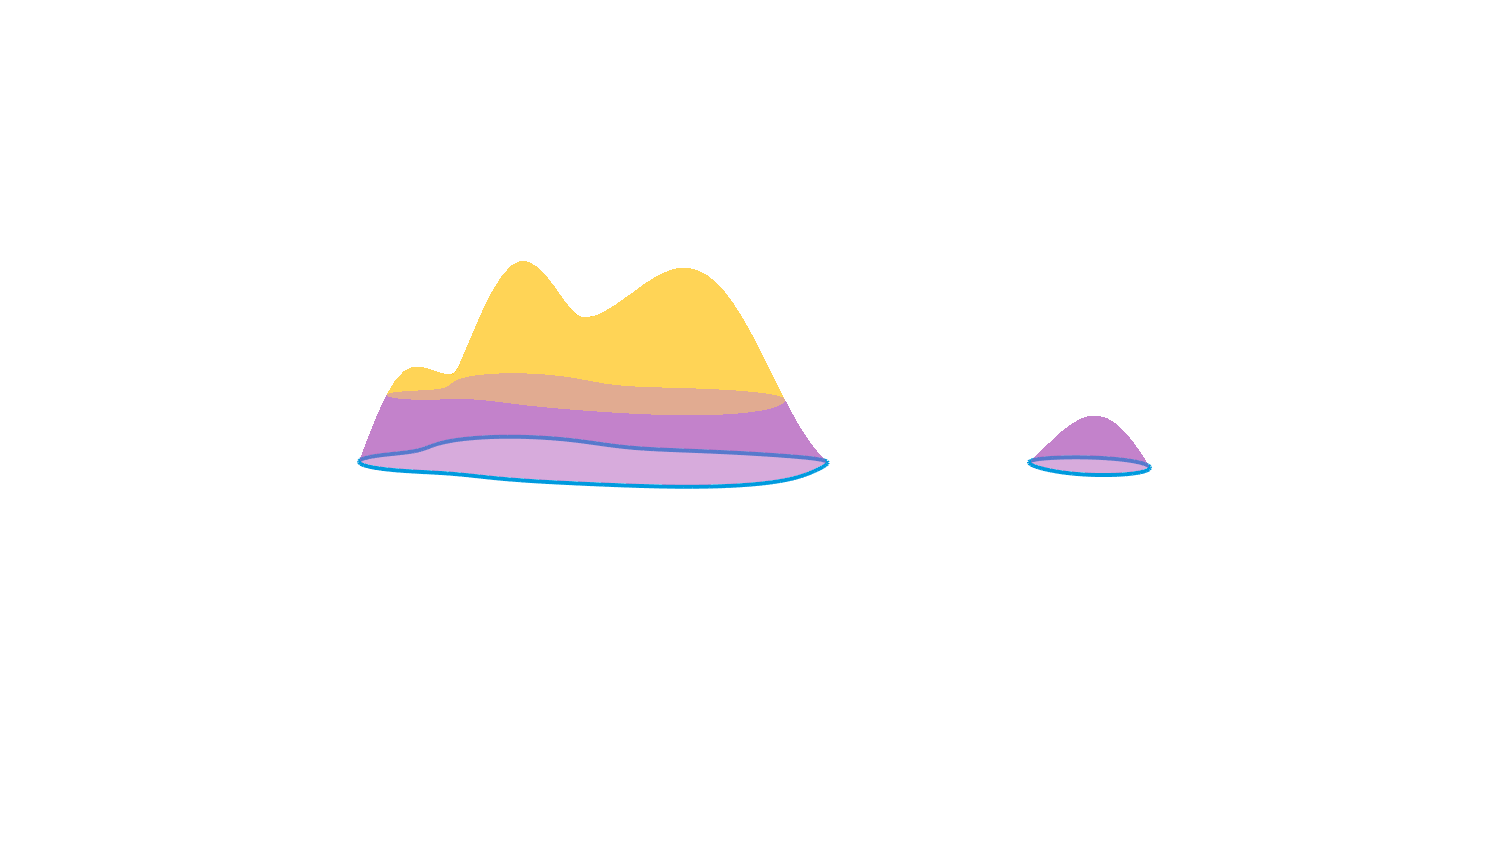
\includegraphics[trim=200 300 200 200, clip, width=0.3\textwidth]{figures/surf/ass1_C_side.png}
  
\includegraphics[trim=200 300 200 200, clip, width=0.3\textwidth]{figures/surf/ass1_D_side.png}
  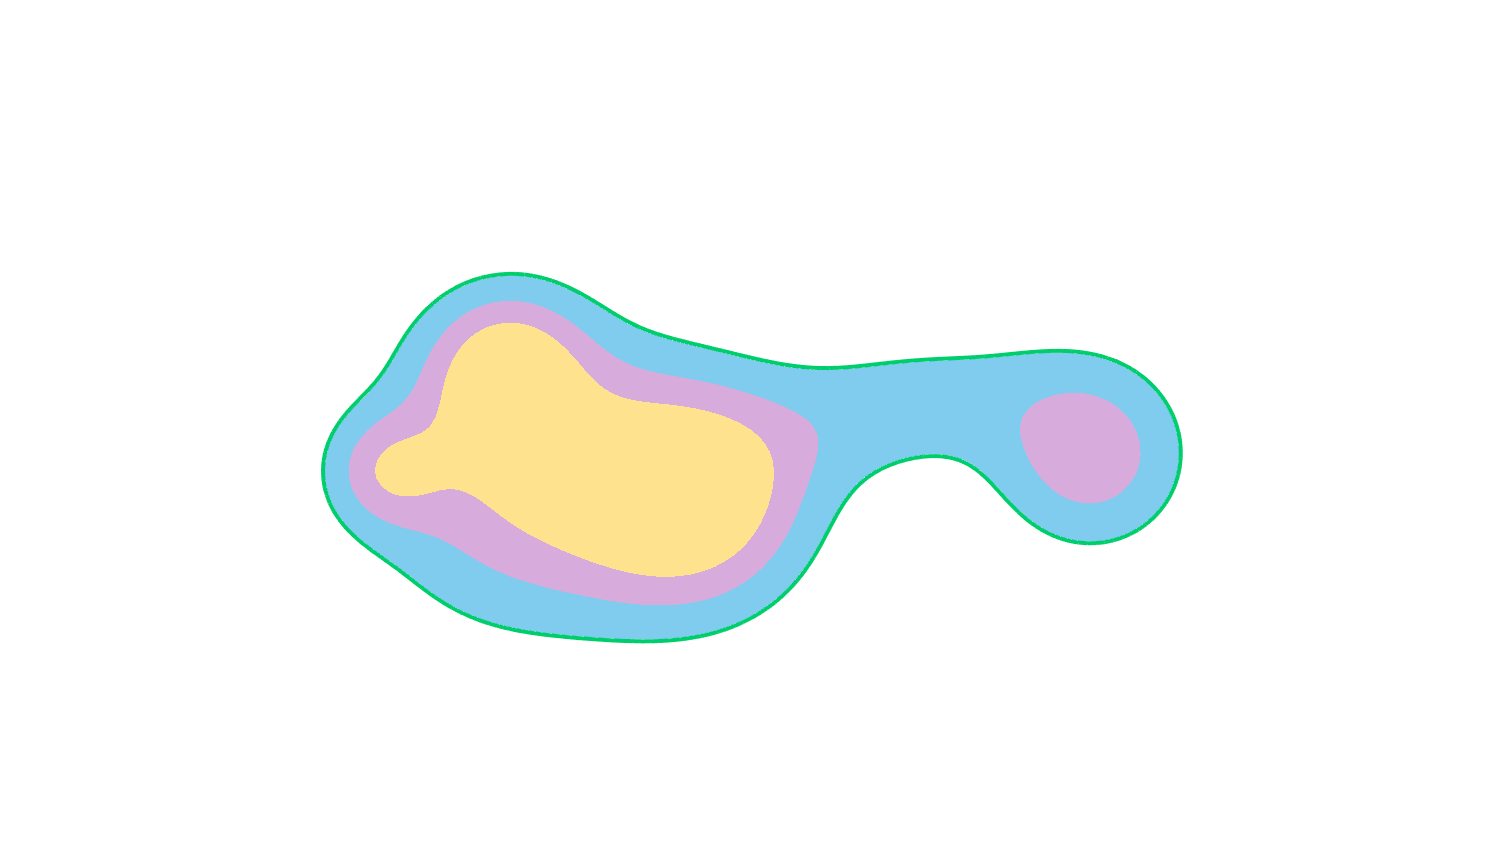
\includegraphics[trim=300 100 200 200, clip, width=0.3\textwidth]{figures/surf/ass2_B_top.png}
  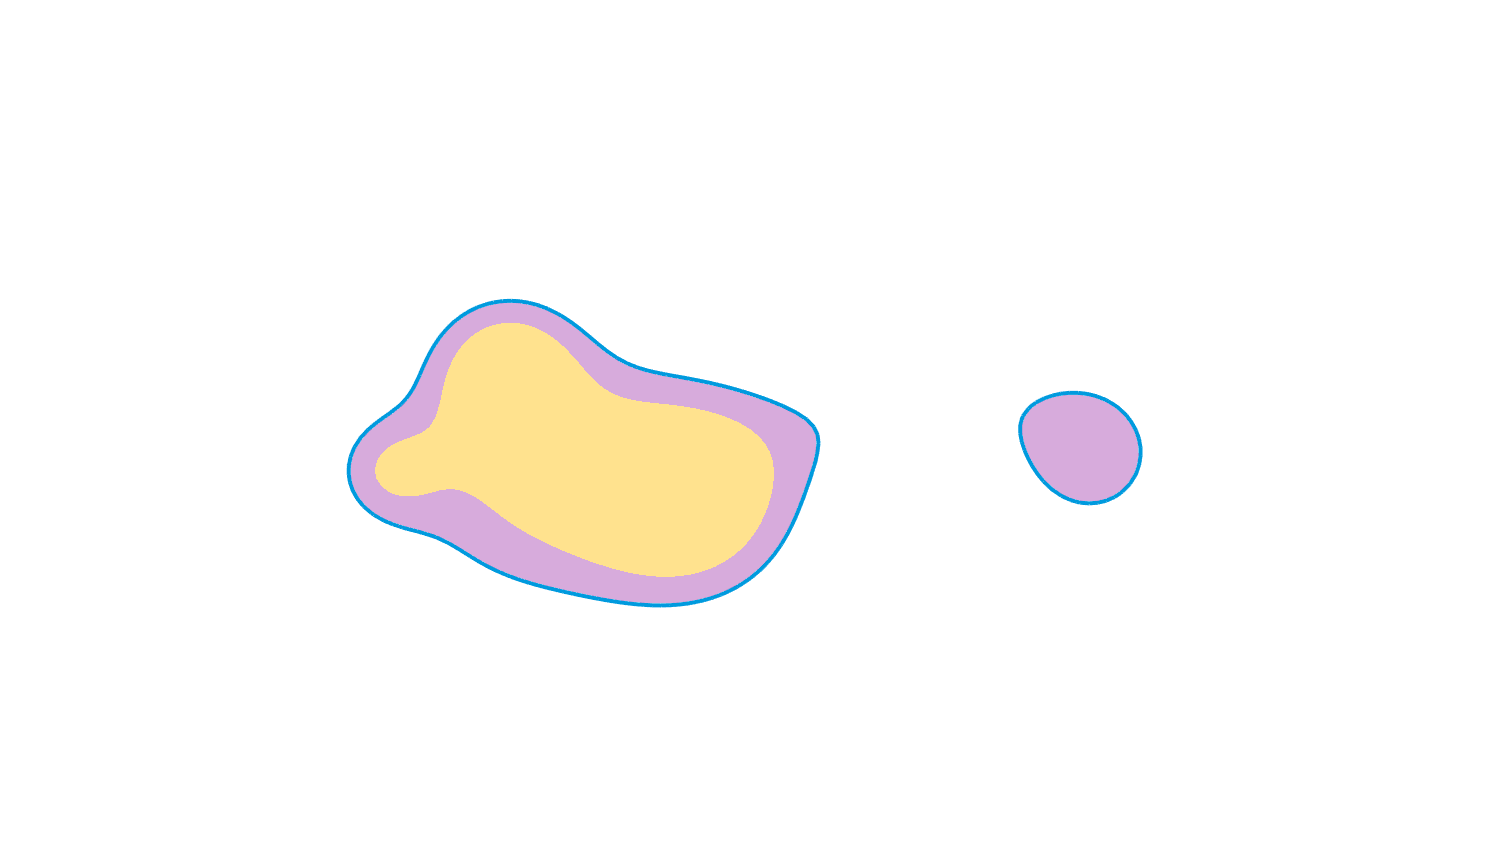
\includegraphics[trim=300 150 300 200, clip, width=0.3\textwidth]{figures/surf/ass1_C_top.png}
  
\includegraphics[trim=300 150 300 200, clip, width=0.3\textwidth]{figures/surf/ass1_D_top.png}
  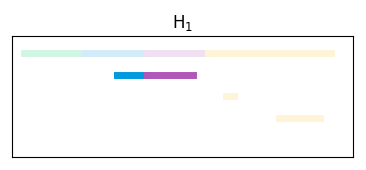
\includegraphics[width=0.5\textwidth]{figures/scalar_barcode_H1-masked.png}
  \caption{The blue level set in the middle does not satisfy either assumption.
    The inclusion from the right is not \emph{surjective} as the smaller component appears in the middle (in the sublevel barcode, a $\hom_{d-1}$ feature dies in the purple region).
    The inclusion to the left is not \emph{injective} as the smaller component is merged with the larger (in the sublevel barcode, a $\hom_{d-1}$ feature is born in the blue region).}\label{fig:assumption1}
\end{figure}

\begin{lemma}\label{lem:assumption2}
  If $\hom_0(D\setminus B_\omega\hookrightarrow D\setminus B_{\omega+c(\delta+\zeta)})$ is injective and each component of $D\setminus B_\omega$ contains a point in $P$ then $\dim~\hom_0(\rips^\delta(P\setminus Q_{\omega-c\zeta})) \geq \dim~\hom_0(D\setminus B_\omega)$.
\end{lemma}

\paragraph*{Nerves and Duality}

The Nerve Theorem states that for a good open cover $\U$ of a space $X$ the inclusion map from the \emph{Nerve} of the cover to the space $\N(\U)\hookrightarrow X$ is a homotopy equivalence.\footnote{In a good open cover every nonempty intersection of sets in the cover is contractible.}
The Persistent Nerve Lemma~\cite{chazal08towards} states that this homotopy equivalence commutes with inclusion on the level of homology.
The standard proof of the Nerve Theorem~\cite{kozlov07combinatorial}, and therefore the Persistent Nerve Lemma, extends directly to pairs of good open covers $(\U, \V)$ of pairs $(X, Y)$ such that $\V$ is a subcover of $\U$.\footnote{$\{V_i\}_{i\in I}$ is a subcover of $\{U_i\}_{i\in I}$ if $V_i\subseteq U_i$ for all $i\in I$.}

Recalling the definition of the strong convexity radius $\varrho_D$ (see Chazal et al.~\cite{chazal09analysis}) $\U$ is a good open cover whenever $\varrho_D > \e$.
As the \v Cech complex is the Nerve of a cover by metric balls we will let $\N_z^\e : \hom_k(\cech^\e(P,Q_z))\to \hom_k(P^\e, Q_z^\e)$ denote the isomorphism on homology provided by the Nerve Theorem for all $z\in\R$, $\e < \varrho_D$ and $k$.

Under certain conditions Alexander Duality provides an isomorphism between the $k$th relative cohomology of a compact pair in an orientable $d$-manifold $\X$ with the $d - k$ dimensional homology of their complements in $\X$ (see Spanier~\cite{spanier1989algebraic}).
For finitely generated (co)homology over a field the Universal Coefficient Theorem can be used with Alexander Duality to show $\hom_d(P^\e,Q_z^\e)\cong\hom_0(D\setminus Q_z^\e, D\setminus P^\e)$.
 % give a natural isomorphism $\xi_z^\e : \hom_d(P^\e,Q_z^\e)\to \hom_0(D\setminus Q_z^\e, D\setminus P^\e)$.\footnote{For the construction of this isomorphism see the \fullversion.}
This isomorphism holds in the specific case when $P^\e\subseteq \intr_\X(D)$ and $D\setminus P^\e$, $D\setminus Q_z^\e$ are locally contractible.
We therefore provide the following definition for ease of exposition.
\begin{definition}[$(\omega, \delta,\zeta)$-Sample]
  For $\zeta\geq \delta > 0$, $\omega\in\R$, and a $c$-Lipschitz function $f: D\to \R$ a finite point set $P\subset D$ is said to be an \textbf{$(\omega, \delta, \zeta)$-sample} of $f$ if \begin{itemize}
    \item $P^\delta\subset\intr_\X(D)$ and
    \item $D\setminus P^\delta$, $D\setminus Q_{\omega-c\zeta}^\delta$, and $D\setminus Q_{\omega+c\delta}^\delta$ are locally path connected in $\X$.
  \end{itemize}
\end{definition}

\begin{theorem}[Algorithmic TCC]\label{thm:algo_tcc}
  Let $\X$ be an orientable $d$-manifold and let $D$ be a compact subset of $\X$.
  Let $f : D\to\R$ be $c$-Lipschitz function and $\omega\in\R$, $\delta\leq\zeta < \varrho_D$ be constants such that $B_{\omega - c(\zeta +\delta)}$ surrounds $D$ in $\X$.
  Let $P$ be an $(\omega, \delta,\zeta)$-sample of $f$ such that every component of $D\setminus B_\omega$ contains a point in $P$.
  Suppose $\hom_0(D\setminus B_{\omega+c(\delta+\zeta)}\hookrightarrow D\setminus B_\omega)$ is surjective and $\hom_0(D\setminus B_\omega\hookrightarrow D\setminus B_{\omega-c(\delta+\zeta)})$ is injective.

   If $\rk~\hom_d(\rips^\delta(P, Q_{\omega -c\zeta})\hookrightarrow \rips^{2\delta}(P, Q_{\omega+c\delta})) \geq \dim~\hom_0(\rips^\delta(P\setminus Q_{\omega-c\zeta}))$ then $D\setminus B_\omega\subseteq P^\delta$ and $Q_{\omega-c\zeta}^\delta$ surrounds $P^\delta$ in $D$.
\end{theorem}
\begin{proof}
  Let $q : \hom_d(P^\delta, Q_{\omega-c\zeta}^\delta)\to \hom_d(P^\delta, Q_{\omega+c\delta}^\delta)$,
  $q_{\cech} : \hom_d(\cech^{\delta}(P, Q_{\omega-c\zeta}))\to\hom_d(\cech^{\delta}(P, Q_{\omega+c\delta}))$, and
  $q_{\rips} : \hom_d(\rips^{\delta}(P, Q_{\omega-c\zeta}))\to\hom_d(\rips^{2\delta}(P, Q_{\omega+c\delta}))$ be induced by inclusion.
  Then $\rk~q_{\cech} \geq\rk~q_{\rips}$ as $q_{\rips}$ factors through $q_{\cech}$ by the Rips-\v Cech interleaving.
  Moreover, $\rk~q = \rk~q_{\cech}$ by the Persistent Nerve Lemma, so $\rk~q\geq \rk~q_{\rips}$.
  As we have assumed $\hom_0(D\setminus B_\omega\hookrightarrow D\setminus B_{\omega-c(\delta+\zeta)})$ is injective Lemma~\ref{lem:assumption2} implies $\dim~\hom_0(\rips^\delta(P\setminus Q_{\omega-c\zeta}))\geq \dim~\hom_0(D\setminus B_\omega)$.
  Because $P$ is an $(\omega, \delta, \zeta)$-sample of $f$ we have $\hom_d(P^\delta, Q_{\omega-c\zeta}^\delta)\cong \hom_0(D\setminus Q_{\omega-c\zeta}^\delta, D\setminus P^\delta)$ and $\hom_d(P^\delta, Q_{\omega+c\delta}^\delta)\cong \hom_0(D\setminus Q_{\omega-2c\delta}^\delta, D\setminus P^\delta)$ so $\rk~i\geq \rk~q$ by Alexander Duality and the Universal Coefficient Theorem.
  So, by our hypothesis that $\rk~q_{\rips}\geq\dim~\hom_0(\rips^\delta(P\setminus Q_{\omega-c\zeta}))$ we have $\rk~i\geq\dim~\hom_0(D\setminus B_\omega)$.

  Because $j : \hom_0(D\setminus B_{\omega+c(\delta+\zeta)}\hookrightarrow D\setminus B_\omega)$ is surjective by hypothesis $\rk~j = \dim~\hom_0(D\setminus B_\omega)$ so $\rk~j\geq \rk~i$ by Lemma~\ref{lem:psurj}.
  As we have shown $\rk~i\geq \dim~\hom_0(D\setminus B_\omega)$ it follows that $\rk~j = \rk~i$.
  Because $P$ is a finite point set we know that $\im~i$ is finite-dimensional and, because $\rk~i = \rk~j$, $\im~j=\hom_0(\overline{B_\omega}, \overline{D})$ is finite dimensional as well.
  So $\im~j$ is isomorphic to $\im~i$ as a subspace of $\hom_0(\overline{Q_{\omega-c\zeta}^\delta}, \overline{P^\delta})$ which, because $j$ is surjective, requires the map $\ell$ to be injective.
  Therefore $D\setminus B_\omega\subseteq P^\delta$ and $Q_{\omega-c\zeta}^\delta$ surrounds $P^\delta$ in $D$ by Lemma~\ref{lem:coverage}.
\end{proof}

% Because this isomorphism is natural with respect to maps induced by inclusion, and isomorphism provided by the Nerve Theorem commutes with maps induced by inclusion the composition $\xi\N_w^\e := \xi_w^\e\circ\N_w^\e$ gives an isomorphism that commutes with maps induced by inclusion for all $w\in\R$ and $\e < \varrho_D$.

% \begin{theorem}[Algorithmic TCC]\label{thm:algo_tcc}
%   Let $\X$ be an orientable $d$-manifold and let $D$ be a compact subset of $\X$.
%   Let $f : D\to\R$ be $c$-Lipschitz function and $\omega\in\R$, $\delta\leq\zeta < \varrho_D$ be constants such that $B_{\omega - c(\zeta +\delta)}$ surrounds $D$ in $\X$.
%   Let $P$ be an $(\omega, \delta,\zeta)$-sample of $f$ such that every component of $D\setminus B_\omega$ contains a point in $P$.
%   Suppose $\hom_0(D\setminus B_{\omega+c(\delta+\zeta)}\hookrightarrow D\setminus B_\omega)$ is surjective and $\hom_0(D\setminus B_\omega\hookrightarrow D\setminus B_{\omega-c(\delta+\zeta)})$ is injective.
%
%    If $\rk~\hom_d(\rips^\delta(P, Q_{\omega -c\zeta})\hookrightarrow \rips^{2\delta}(P, Q_{\omega+c\delta})) \geq \dim~\hom_0(\rips^\delta(P\setminus Q_{\omega-c\zeta}))$ then $D\setminus B_\omega\subseteq P^\delta$ and $Q_{\omega-c\zeta}^\delta$ surrounds $P^\delta$ in $D$.
% \end{theorem}
% \begin{proof}
%   % We have the following commutative diagram
%   % \[\begin{tikzcd}
%   %   \hom_d(\cech^\delta(P, Q_{\omega-c\zeta})) \arrow{r}{q_{\cech}}\arrow{d}{\N_{\omega-c\zeta}^{\delta}} &
%   %   \hom_d(\cech^\delta(P, Q_{\omega+c\delta})) \arrow{d}{\N_{\omega-c\zeta}^\delta}\\
%   %   %
%   %   \hom_d(P^\delta, Q_{\omega-c\zeta}^\delta))\arrow{r}{q} &
%   %   \hom_d(P^\delta, Q_{\omega+c\delta}^\delta).
%   % \end{tikzcd}\]
%   % where vertical maps are isomorphisms provided by the Nerve Theorem and horizontal maps are induced by inclusions.
%
%   Because $P$ is an $(\omega, \delta, \zeta)$-sublevel sample we have isomorphisms $\xi\N_{\omega-c\zeta}^\delta$ and $\xi\N_{\omega+c\delta}^\delta$ that commute with $q_{\cech} : \hom_d(\cech^{\delta}(P, Q_{\omega-c\zeta}))\to\hom_d(\cech^{2\delta}(P, Q_{\omega+c\delta}))$ and $i : \hom_0(D\setminus Q_{\omega+c\delta}^\delta, D\setminus P^\delta)\to \hom_0(D\setminus Q_{\omega-c\zeta}^\delta, D\setminus P^\delta)$.
%   Let $q_{\rips} : \hom_d(\rips^{\delta}(P, Q_{\omega-c\zeta}))\to\hom_d(\rips^{2\delta}(P, Q_{\omega+c\delta}))$ be induced by inclusion.
%   Then $\rk~q_{\cech} \geq\rk~q_{\rips}$ as $q_{\rips}$ factors through $q_{\cech}$.
%   As we have assumed $\hom_0(D\setminus B_\omega\hookrightarrow D\setminus B_{\omega-c(\delta+\zeta)})$ Lemma~\ref{lem:assumption2} implies $\dim~\hom_0(\rips^\delta(P\setminus Q_{\omega-c\zeta}))\geq \dim~\hom_0(D\setminus B_\omega)$.
%   It follows that, whenever $\rk~q_{\rips} \geq \dim~\hom_0(\rips^\delta(P\setminus Q_{\omega-c\zeta}))$, we have
%   \[ \rk~i = \rk~q_{\cech} \geq \rk~q_{\rips} \geq \dim~\hom_0(\rips^\delta(P\setminus Q_{\omega-c\zeta})) \geq \dim~\hom_0(D\setminus B_\omega).\]
%
%   Because $j$ is surjective by hypothesis $\rk~j = \dim~\hom_0(\overline{B_\omega},\overline{D}) = \dim~\hom_0(D\setminus B_\omega)$ so $\rk~j\geq \rk~i$ by Lemma~\ref{lem:psurj}.
%   As we have shown $\rk~i\geq \dim~\hom_0(D\setminus B_\omega)$ it follows that $\rk~j = \rk~i$.
%   Because $P$ is a finite point set we know that $\im~i$ is finite-dimensional and, because $\rk~i = \rk~j$, $\im~j=\hom_0(\overline{B_\omega}, \overline{D})$ is finite dimensional as well.
%   So $\im~j$ is isomorphic to $\im~i$ as a subspace of $\hom_0(\overline{Q_{\omega-c\zeta}^\delta}, \overline{P^\delta})$ which, because $j$ is surjective, requires the map $\ell$ to be injective.
%   Therefore $D\setminusB_\omega\subseteq P^\delta$ and $Q_{\omega-c\zeta}^\delta$ surrounds $P^\delta$ in $D$ by Lemma~\ref{lem:coverage}.
%   %, Lemma~\ref{lem:cov_surrounds}.
%   % As $j : \hom_0(D\setminus B_{\omega+c(\delta+\zeta)})\to \hom_0(D\setminus B_\omega)$ is surjective by assumption $\rk~j = \dim~\hom_0(D\setminus B_\omega)$, so $D\setminus B_\omega\subseteq P^\delta$ and $Q_{\omega-c\zeta}^\delta$ surrounds $P^\delta$ in $D$ by Theorem~\ref{thm:geo_tcc} as desired.
% \end{proof}


\section{From Coverage Testing to the Analysis of Scalar Fields}\label{sec:middle}
% !TeX root = ../main.tex

Because the TCC only confirms coverage of a \emph{superlevel} set $D\setminus B_\omega$, we cannot guarantee coverage of the entire domain.
Indeed, with sufficient smoothness assumptions on the boundary we could compute the persistent homology of the \emph{restriction} of $f$ to the superlevel set we cover in the standard way~\cite{chazal09analysis}.
Instead, we will approximate the persistent homology of the sublevel set filtration \emph{relative to} the sublevel set $B_\omega$.
In the next section we will discuss an interpretation of the relative diagram that is motivated by examples in Section~\ref{sec:experiments}.

We will first introduce the notion of an extension which will provide us with maps on relative homology induced by inclusion via excision.
However, even then, a map that factors through our pair $(D, B_\omega)$ is not enough to prove an interleaving of persistence modules by inclusion directly.
To address this we impose conditions on sublevel sets near $B_\omega$ which generalize the assumptions made in the TCC.

\subsection{Extensions and Image Persistence Modules}

Suppose $D$ is a subspace of a topological space $X$.
We define the extension of a surrounding pair in $D$ to a surrounding pair in $X$ with isomorphic relative homology.

\begin{definition}[Extension]
  If $V$ surrounds $U$ in a subspace $D$ of $X$ let $\ext{V} := V\sqcup (D\setminus U)$ denote the (disjoint) union of the separating set $V$ with the complement of $U$ in $D$.
  The \textbf{extension of $(U, V)$ in $D$} is the pair $(D, \ext{V}) = (U\sqcup (D\setminus U), V\sqcup (D\setminus U)).$
\end{definition}

Lemma~\ref{lem:surround_and_cover} states that we can use these extensions to interleave a pair $(U, V)$ with a sequence of subsets of $(D, B)$.
Lemma~\ref{lem:excision} states that we can apply excision to the relative homology groups in order to get equivalent maps on homology that are induced by inclusions.

\begin{lemma}\label{lem:surround_and_cover}
  Suppose $V$ surrounds $U$ in $D$ and $B'\subseteq B\subset D$.

  If $D\setminus B\subseteq U$ and $U\cap B'\subseteq V\subseteq B'$ then $B'\subseteq \ext{V}\subseteq B$.
\end{lemma}

\begin{lemma}\label{lem:excision}
  Let $(U, V)$ be an open surrounding pair in a subspace $D$ of $X$.

  Then $\hom_k((U\cap A, V)\hookrightarrow (A, \ext{V}))$ is an isomorphism for all $k$ and $A\subseteq D$ with $\ext{V}\subset A$.
\end{lemma}

The TCC uses a nested pair of spaces in order to filter out noise introduced by the sample.
This same technique is used to approximate the persistent homology of a scalar field~\cite{chazal09analysis}.
As modules, these nested pairs are the images of homomorphisms between homology groups induced by inclusion, which we refer to as image persistence modules.
For a full background on persistence modules, shifted homomorphisms, and interleavings of persistence modules see Chazal et al.~\cite{chazal13structure}.

\begin{definition}[Image Persistence Module]
  The \textbf{image persistence module} of a homomorphism $\Gamma\in\Hom(\UU,\VV)$ is the family of subspaces $\{\Gamma_\alpha :=\im~\gamma_\alpha\}$ in $\VV$ along with linear maps $\{\gamma_\alpha^\beta := v_\alpha^\beta\rest_{\im~\gamma_\alpha} : \Gamma_\alpha\to\Gamma_\beta\}$ and will be denoted by $\im~\Gamma$.
\end{definition}

For a homomorphism $\Gamma\in\Hom(\UU, \VV)$ let $\Gamma[\delta]\in \Hom^{\delta}(\UU, \VV)$ denote the shifted homomorphism defined to be the family of linear maps $\{\gamma_\alpha[\delta] := v_\alpha^\delta\circ \gamma_\alpha : U_\alpha\to V_{\alpha+\delta}\}$.
While we will primarily work with homomorphisms of persistence modules induced by inclusions, in general, defining homomorphisms between images simply as subspaces of the codomain is not sufficient.
Instead, we require that homomorphisms between image modules commute not only with shifts in scale, but also with the functions themselves.

\begin{definition}[Image Module Homomorphism]
  Given $\Gamma\in\Hom(\UU,\VV)$ and $\Lambda\in\Hom(\S,\T)$ along with $(F,G)\in\Hom^\delta(\UU,\S)\times\Hom^\delta(\VV,\T)$ let $\Phi(F, G) : \im~\Gamma\to\im~\Lambda$ denote the family of linear maps $\{\phi_\alpha := g_\alpha\rest_{\Gamma_\alpha} : \Gamma_\alpha\to\Lambda_{\alpha+\delta}\}$.
  $\Phi(F, G)$ is an \textbf{image module homomorphism of degree $\delta$} if the following diagram commutes for all $\alpha\leq\beta$.
  \begin{equation}\label{dgm:image_homomorphism}
    \begin{tikzcd}[column sep=large]
        U_\alpha\arrow{r}{\gamma_\alpha[\beta-\alpha]}\arrow{d}{f_\alpha} &
      V_\beta\arrow{d}{g_\beta}\\
      %
      S_{\alpha+\delta}\arrow{r}{\lambda_{\alpha+\delta}[\beta-\alpha]} &
      T_{\beta +\delta}
  \end{tikzcd}\end{equation}
  The space of image module homomorphisms of degree $\delta$ between $\im~\Gamma$ and $\im~\Lambda$ will be denoted $\Hom^\delta(\im~\Gamma,\im~\Lambda)$.
\end{definition}

\begin{lemma}\label{lem:image_composition}
  Suppose $\Gamma\in\Hom(\UU,\VV)$, $\Lambda\in\Hom(\S,\T)$, and $\Lambda'\in\Hom(\S',\T')$.
  If $\Phi(F, G)\in\Hom^\delta(\im~\Gamma, \im~\Lambda)$ and $\Phi'(F', G')\in\Hom^{\delta'}(\im~\Lambda, \im~\Lambda')$ then $\Phi''(F'\circ F, G'\circ G) := \Phi'\circ\Phi\in\Hom^{\delta+\delta'}(\im~\Gamma,\im~\Lambda')$.
\end{lemma}

\paragraph*{Partial Interleavings of Image Modules}

Image module homomorphisms introduce a direction to the traditional notion of interleaving.
As we will see, our interleaving via Lemma~\ref{thm:interleaving_main} involves partially interleaving an image module to two other image modules whose composition is isomorphic to our target.

\begin{definition}[Partial Interleaving of Image Modules]
  An image module homomorphism $\Phi(F, G)$ is a \textbf{partial $\delta$-interleaving of image modules}, and denoted $\Phi_M(F, G)$, if there exists $M\in\Hom^\delta(\S,\VV)$ such that $\Gamma[2\delta] = M\circ F$ and $\Lambda[2\delta] = G\circ M$.
\end{definition}

Lemma~\ref{thm:interleaving_main} uses partial interleavings of a map $\Lambda$ with $\UU\to\VV$ and $\VV\to\W$ along with the hypothesis that $\im(\UU\to \W)$ is isomorphic to $\VV$ to interleave $\im~\Lambda$ with $\VV$.
When applied, this hypothesis will be satisfied by assumptions on our sublevel set similar to those made in the TCC.

\begin{lemma}\label{thm:interleaving_main}
  Suppose $\Gamma\in\Hom(\UU,\VV)$, $\Pi\in\Hom(\VV,\W)$, and $\Lambda\in\Hom(\S, \T)$.

  If $\Phi_M(F, G)\in\Hom^\delta(\im~\Gamma, \im~\Lambda)$ and $\Psi_G(M, N)\in\Hom^\delta(\im~\Lambda, \im~\Pi)$ are partial $\delta$-interleavings of image modules such that $\Gamma$ is a epimorphism and $\Pi$ is a monomorphism then $\im~\Lambda$ is $\delta$-interleaved with $\VV$.
\end{lemma}

% !TeX root = ../main.tex

\subsection{Proof of the Interleaving}

For $z,\alpha\in\R$ let $\DD{z}^k$ denote the $k$th persistent (relative) homology module of the filtration $\{(D\subi{z}{\alpha},B_z)\}_{\alpha\in\R}$ with respect to $B_z$, and let $\PP{z}{\e,k}$ denote the $k$th persistent (relative) homology module of $\{(P\subi{z}{\alpha}^\e,Q_z^\e)\}_{\alpha\in\R}$.
Similarly, let $\CPP{z}{\e,k}$ and $\RPP{z}{\e,k}$ denote the corresponding \v Cech and Rips filtrations, respectively.
We will omit the dimension $k$ and write $\DD{z}$ (resp. $\PP{z}{\e}$) if a statement holds for all dimensions.
If $Q_z^\delta$ surrounds $P^\delta$ in $D$ let $\ext{\PP{z}{\e}}$ denote the $k$th persistent homology module of the filtration of extensions $\{(\ext{P\subi{z}{\alpha}^\e},\ext{Q_z^\e})\}$ for any $\e\geq\delta$, where $\ext{P\subi{z}{\alpha}^\e} = P\subi{z}{\alpha}^\e \cup (D\setminus P^\delta)$.

Lemma~\ref{lem:inclusions} follows directly from the definition of truncated sublevel sets.
This is used to extend Lemma~\ref{lem:surround_and_cover} to persistence modules in Lemma~\ref{lem:inclusion_hom} in order to provide a sequence of shifted homomorphisms $\DD{\omega-3c\delta}\xrightarrow{F}\E\PP{\omega-2c\delta}{\e}\xrightarrow{M}\DD{\omega}\xrightarrow{G}\E\PP{\omega+c\delta}{2\e}\xrightarrow{N}\DD{\omega+5c\delta}$ of varying degree.
These homomorphisms are then combined with those given by the Nerve Theorem and the Rips-\v Cech interleaving in Lemma~\ref{lem:partial_interleaving} to obtain partial interleavings required for our proof of Theorem~\ref{thm:interleaving_main_2}.

\begin{lemma}\label{lem:inclusions}
  If $\delta\leq\e$ and $t,\alpha\in\R$ then $P^\delta\cap D\subi{t-c\e}{\alpha-c\e}\subseteq P\subi{t}{\alpha}^\e\subseteq D\subi{t+c\e}{\alpha+c\e}$.
\end{lemma}

\begin{lemma}\label{lem:inclusion_hom}
  Let $s + 3c\delta\leq t + 2c\delta\leq u\leq v-c\delta\leq w-5c\delta$ and $\e\in [\delta,2\delta]$.
  If $Q_{t}^\delta$ surrounds $P^\delta$ in $D$ and $D\setminus B_u\subseteq P^\delta$ then the following homomorphisms are induced by inclusions:
  \[(F, G)\in \Hom^{c\delta}(\DD{s}, \E\PP{t}{\e})\times \Hom^{2c\delta}(\DD{u}, \E\PP{v}{2\e}),\ (M, N)\in \Hom^{c\e}(\E\PP{t}{\e},\DD{u})\times\Hom^{2c\e}(\E\PP{v}{2\e}, \DD{w}).\]
\end{lemma}

\begin{lemma}\label{lem:partial_interleaving}
  For $\delta < \varrho_D$ and $s + 3c\delta\leq t + 2c\delta\leq u\leq v-c\delta\leq w-5c\delta$ let
  $\Gamma\in\Hom(\DD{s},\DD{u})$,
  $\Pi\in\Hom(\DD{u},\DD{w})$, and
  $\Lambda\in\Hom(\RPP{t}{2\delta}, \RPP{v}{4\delta})$ be induced by inclusions.

  If $Q_{t}^\delta$ surrounds $P^\delta$ in $D$ and $D\setminus B_u\subseteq P^\delta$ then there is a partial $2c\delta$ interleaving $\Phi^*\in\Hom^{2c\delta}(\im~\Gamma, \im~\Lambda)$ and a partial $4c\delta$ interleaving $\Psi^*\in\Hom^{4c\delta}(\im~\Lambda, \im~\Pi)$.
\end{lemma}
\begin{proof}
  Because the shifted homomorphisms provided by Lemma~\ref{lem:inclusion_hom} are all induced by inclusions the following diagram commutes for all $\alpha\leq\beta$.
  So we have image module homomorphisms $\Phi(F, G)\in\Hom^{2c\delta}(\im~\Gamma, \im~C\circ A)$ and $\Psi(M, N)\in\Hom^{4c\delta}(\im~E\circ C, \im~\Pi)$.
  \[\begin{tikzcd}
      \hom_k(D\subi{s}{\alpha-2c\delta}, B_s) \arrow{r}{f_{\alpha-2c\delta}}\arrow{d}{\gamma_{\alpha-2c\delta}[\beta-\alpha]} &
      \hom_k(\E P\subi{t}{\alpha}^\delta, \E Q_t^\delta)\arrow{d}{c_\alpha[\beta-\alpha]\circ a_\alpha}\\
      %
      \hom_k(D\subi{u}{\beta-2c\delta}, B_u)\arrow{r}{g_{\beta-2c\delta}} &
      \hom_k(\E P\subi{v}{\beta}^{2\delta}, \E Q_v^{2\delta})
    \end{tikzcd}
    \begin{tikzcd}
      \hom_k(\E P\subi{t}{\alpha}^{2\delta}, \E Q_t^{2\delta})\arrow{d}{e_\beta\circ c_\alpha[\beta-\alpha]}\arrow{r}{m_{\alpha}} &
      \hom_k(D\subi{u}{\alpha+4c\delta}, B_u)\arrow{d}{\gamma_{\alpha+4c\delta}[\beta-\alpha]}\\
      %
      \hom_k(\E P\subi{v}{\beta}^{4\delta}, \E Q_v^{4\delta})\arrow{r}{n_\beta} &
      \hom_k(D\subi{w}{\beta+4c\delta}, B_w)
    \end{tikzcd}\]

  Because the isomorphisms provided by Lemma~\ref{lem:excision} are given by excision they are induced by inclusion, and therefore give isomorphisms $\E_z^\e \in \Hom(\PP{z}{\e},\ext{\PP{z}{\e}})$ for any $z\in\R$ such that $Q_z^\e$ surrounds $P^\delta$ in $D$.
  For any $\e < \varrho_D$ we have isomorphisms $\N_z^\e\in\Hom(\CPP{z}{\e}, \PP{z}{\e})$ that commute with maps induced by inclusions by the Persistent Nerve Lemma.
  So the compositions $\E_z^\e\circ \N_z^\e$ are isomorphisms that commute with maps induced by inclusion as well.
  These compositions, along with the Rips-\v Cech interleaving, provide maps $\E\PP{t}{\delta}\xrightarrow{F'}\RPP{t}{2\delta}\xrightarrow{M'} \E\PP{t}{2\delta}$ and $\E\PP{v}{2\delta}\xrightarrow{G'}\RPP{v}{4\delta}\xrightarrow{N'} \E\PP{v}{4\delta}$ that commute with maps induced by inclusions.
  So we have the following commutative diagram:
  %
  \begin{equation}
    \begin{tikzcd}
      \E\PP{t}{\delta}\arrow{rr}{A}\arrow{dr}{F'} & &
      \E\PP{t}{2\delta}\arrow{r}{C} &
      \E\PP{v}{2\delta}\arrow{rr}{E}\arrow{dr}{G'} & &
      \E\PP{v}{4\delta}\\
      %
      & \RPP{t}{2\delta}\arrow{ur}{M'}\arrow[to=RV, "\Lambda"] & &
      & |[alias=RV]|\RPP{v}{4\delta}\arrow{ur}{N'} &
    \end{tikzcd}
  \end{equation}
  %
  That is, we have image module homomorphisms $\Phi'(F', G')$ and $\Psi'(M', N')$ such that $A = M'\circ F'$, $E = N'\circ G'$, and $\Lambda = G'\circ C\circ M'$.
  Because all maps are induced by inclusions or commute with maps induced by inclusions $\Phi^* = \Phi'\circ \Phi\in\Hom^{2c\delta}(\im~\Gamma, \im~\Lambda)$ and $\Psi^* = \Psi\circ\Psi'\in\Hom^{4c\delta}(\im~\Lambda, \im~\Pi)$ by Lemm~\ref{lem:image_composition}.

  Because $G,M,C$ are induced by inclusions $C[3c\delta] = G\circ M$, so $\Lambda[3c\delta] = G'\circ C[3c\delta]\circ M' = G'\circ (G\circ M)\circ M'$ as $G', M'$ commute with maps induced by inclusions.
  In the same way, $\Gamma[3c\delta] = M\circ (A\circ F) = M\circ (M'\circ F')\circ F$ and $\Pi[5c\delta] = N\circ (E\circ G) = N\circ (N'\circ G')\circ G$.

  Let $F^*:= F'\circ F$, $G^*:= G'\circ G$, $M^*:=M'\circ M$, and $N^*:=N'\circ N$.
  So $\Phi^*_{M^*}$ is a partial $2c\delta$ interleaving as $\Gamma[3c\delta] = M^*\circ F^*$ and $\Lambda[3c\delta] = G^*\circ M^*$, and $\Psi^*_{G^*}$ is a partial $4c\delta$ interleaving as $\Lambda[3c\delta] = G^*\circ M^*$ and $\Pi[5c\delta] = N^*\circ G^*$.
\end{proof}

The partial interleavings given by Lemma~\ref{lem:partial_interleaving}, along with assumptions that imply $\im(\DD{\omega-3c\delta}\to \DD{\omega+5c\delta})\cong \DD{\omega}$, provide the proof of Theorem~\ref{thm:interleaving_main_2} by Lemma~\ref{thm:interleaving_main}.

\begin{theorem}\label{thm:interleaving_main_2}
  Let $\X$ be a $d$-manifold, $D\subset\X$ and $f : D\to\R$ be a $c$-Lipschitz function.
  Let $\omega\in\R$, $\delta < \varrho_D/4$ be constants such that $B_{\omega-3c\delta}$ surrounds $D$ in $\X$.
  Let $P\subset D$ be a finite subset and suppose $\hom_k(B_{\omega-3c\delta}\hookrightarrow B_\omega)$ is surjective and $\hom_k(B_\omega\hookrightarrow B_{\omega+5c\delta})$ is an isomorphism for all $k$.

  If $D\setminus B_\omega\subseteq P^\delta$ and $Q_{\omega-2c\delta}^\delta$ surrounds $P^\delta$ in $D$ then the $k$th persistent homology module of $\{\rips^{2\delta}(P\subi{\omega-2c\delta}{\alpha}, Q_{\omega-2c\delta})\hookrightarrow \rips^{4\delta}(P\subi{\omega+c\delta}{\alpha}, Q_{\omega+c\delta})\}_{\alpha\in\R}$ is $4c\delta$-interleaved with that of $\{(D\subi{\omega}{\alpha}, B_\omega)\}_{\alpha\in\R}$.
\end{theorem}
\begin{proof}
  Let $\Lambda \in\Hom(\RPP{\omega-2c\delta}{2c\delta}, \RPP{\omega+c\delta}{4c\delta})$, $\Gamma\in\Hom(\DD{\omega-3c\delta}, \DD{\omega})$, and $\Pi\in\Hom(\DD{\omega},\DD{\omega+5c\delta})$ be induced by inclusions.
  Because $\delta < \varrho_D/4$, $D\setminus B_\omega\subseteq P^\delta$ and $Q_{\omega-2c\delta}^\delta$ surrounds $P^\delta$ in $D$ we have a partial $2c\delta$ interleaving $\Phi^*\in\Hom^{2c\delta}(\im~\Gamma, \im~\Lambda)$ and a partial $4c\delta$ interleaving $\Psi^*\in\Hom^{4c\delta}(\im~\Lambda, \im~\Pi)$ by Lemma~\ref{lem:partial_interleaving}.
  As we have assumed that $\hom_k(B_{\omega-3c\delta}\hookrightarrow B_\omega)$ is surjective and $\hom_k(B_\omega)\cong\hom_k(B_{\omega+5c\delta})$ the five-lemma implies $\gamma_\alpha$ is surjective and $\pi_\alpha$ is an isomorphism (and therefore injective) for all $\alpha$.
  So $\Gamma$ is an epimorphism and $\Pi$ is a monomorphism, thus $\im~\Lambda$ is $4c\delta$-interleaved with $\DD{\omega}$ by Lemma~\ref{thm:interleaving_main} as desired.
\end{proof}


\section{Approximation of the Truncated Diagram}\label{sec:truncations}
% !TeX root = ../main.tex

% \paragraph*{Relative, Truncated, and Restricted Persistence Diagrams}

For fixed $\omega\in\R$ we will refer to the persistence diagram associated with the filtration $\{(D\subi{\omega}{\alpha}, B_\omega)\}_{\alpha\in\R}$  as the \textbf{relative diagram} of $f$.
In this section we will relate the relative diagram to the \emph{full} diagram of the sublevel set filtration $\{B_\alpha\}_{\alpha\in\R}$.
Specifically, we define the \textbf{truncated diagram} to be the subdiagram of the full consisting of features born \emph{after} $\omega$.
In the following section we will compare the relative and truncated diagrams to the \textbf{restricted diagram}, defined to be that of the sublevel set filtration of $f\rest_{D\setminus B_\omega}$.%

Note that the truncated sublevel sets $D\subi{\omega}{\alpha}$ are equal to the union of $B_\omega$ and the restricted sublevel sets.
It is in this sense that $B_\omega$ is \emph{static} throughout---it is contained in every sublevel set of the relative filtration.
As we will not have verified coverage in $B_\omega$ we cannot analyze the function in this region directly.
We therefore have two alternatives: \emph{restrict} the domain of the function to $D\setminus B_\omega$, or use relative homology to analyze the function \emph{relative} to this region using excision.

\begin{figure}[htbp]
  \centering
  \begin{minipage}[b]{0.27\textwidth}
    
\includegraphics[trim=200 200 200 100, clip, width=\textwidth]{figures/surf/ass2_C_side.png}\\
    
\includegraphics[trim=200 100 200 200, clip, width=\textwidth]{figures/surf/ass2_C_top.png}
  \end{minipage}
  \begin{minipage}[b]{0.7\textwidth}
    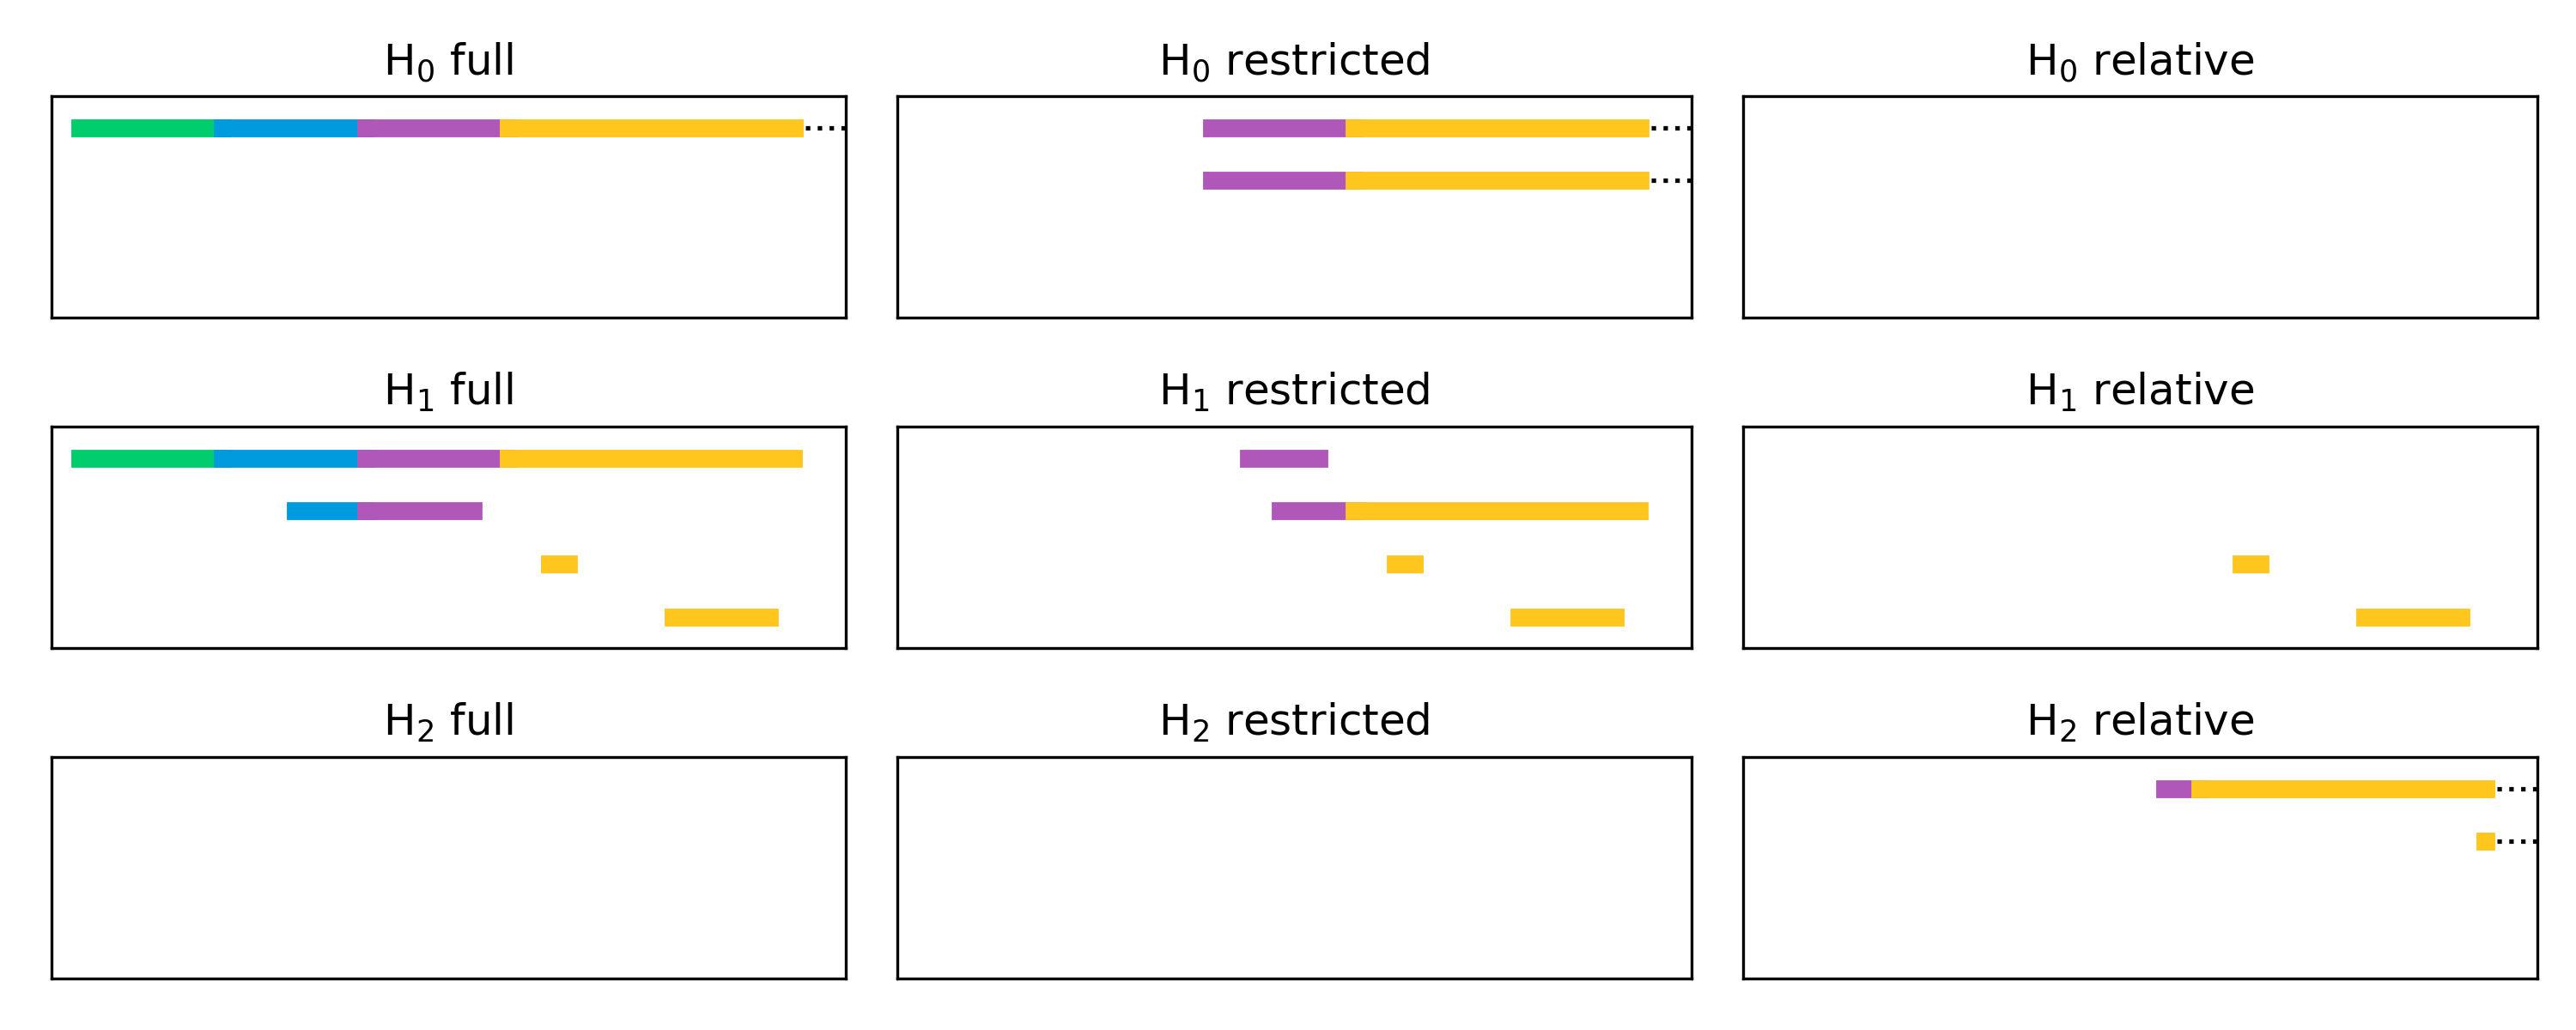
\includegraphics[width=\textwidth]{figures/barcodes/res_rel.png}
  \end{minipage}
  \caption{Full, restricted, and relative barcodes of the function (left).}
\end{figure}

Let $\LL^k$ denote the $k$th persistent homology module of the sublevel set filtration $\{B_\alpha\}_{\alpha\in\R}$.
As in the previous section, let $\DD{\omega}^k$ denote the $k$th persistent (relative) homology module of $\{(D\subi{\omega}{\alpha}, B_\omega)\}_{\alpha\in\R}$.
Throughout we will assume that we are taking homology in a field $\FF$ and that the homology groups $\hom_k(B_\alpha)$ and $\hom_k(D\subi{\omega}{\alpha}, B_\omega)$ are finite dimensional vector spaces for all $k$ and $\alpha\in\R$.
We will use the interval decomposition of $\LL^k$ to give a decomposition of the relative module $\DD{\omega}^k$ in terms of a \emph{truncation} of $\LL^k$.
For fixed $\omega\in\R$ we will define the truncation $\T^k_\omega$ of $\LL^k$ in terms of the intervals decomposing $\LL^k$ that are in $[\omega, \infty)$.

\paragraph*{Truncated Interval Modules}

For an interval $I = [s,t)\subseteq \R$ let $I_+ := [t,\infty)$ and $I_- := (-\infty, s]$.
For $\omega\in\R$ let $\FF_{\omega}^I$ denote the interval module consisting of vector spaces $\{F\subi{\omega}{\alpha}^I\}_{\alpha\in\R}$ and linear maps $\{f\subi{\omega}{\alpha,\beta}^I : F\subi{\omega}{\alpha}^I\to F\subi{\omega}{\beta}^I\}_{\alpha\leq\beta}$ where
\[ F\subi{\omega}{\alpha}^I := \begin{cases} F_\alpha^I&\text{ if } \omega\in I_-\\ 0&\text{ otherwise,}\end{cases}\ \text{ and }\ \ f\subi{\omega}{\alpha,\beta}^I := \begin{cases} f_{\alpha,\beta}^I&\text{ if } \omega\in I_-\\ 0&\text{ otherwise.}\end{cases}\]
For a collection $\I$ of intervals let $\I_\omega := \{I\in\I\mid \omega\in I\}$.

\begin{lemma}\label{lem:decomposition}
  Suppose $\I^k$ and $\I^{k-1}$ are collections of intervals that decompose $\LL^k$ and $\LL^{k-1}$, respectively.
  Then for all $k$ the $k$th persistent homology module of $\{(D\subi{\omega}{\alpha}, B_\omega)\}_{\alpha\in\R}$ is isomorphic to
  \[\bigoplus_{I\in\I^k} \FF_\omega^I \oplus \bigoplus_{I\in \I_\omega^{k-1}} \FF^{I_+}.\]
\end{lemma}
\begin{proof}
  Suppose $\alpha\leq\omega$.
  So $\hom_k(D\subi{\omega}{\alpha}, B_\omega) = 0$ as $D\subi{\omega}{\alpha} = B_\omega\cup B_\alpha$ and $\T^k_\omega = 0$ as $F_\alpha^I = 0$ for any $I\in \I^k$ such that $\omega\in I_-$.
  Moreover, $\omega\in I$ for all $I\in \I_\omega^{k-1}$, thus $F_\alpha^{I_+} = 0$ for all $\alpha\leq\omega$.
  So it suffices to assume $\omega < \alpha$.

  Consider the long exact sequence of the pair $\hom_k(D\subi{\omega}{\alpha}, B_\omega) = \hom_k(B_\alpha, B_\omega)$
  \[ \ldots\to \hom_k(B_\omega)\xrightarrow{p_\alpha^k} \hom_k(B_\alpha)\xrightarrow{q_\alpha^k}\hom_k(D\subi{\omega}{\alpha}, B_\omega)\xrightarrow{r_\alpha^k} \hom_{k-1}(B_\omega)\xrightarrow{p_\alpha^{k-1}}\hom_{k-1}(B_\alpha)\to\ldots\]
  where $\hom_k(B_\alpha) = \bigoplus_{I\in \I^k}F_\alpha^I$, $\hom_k(B_\omega) = \bigoplus_{I\in \I^k}F_\omega^I$, and $p_\alpha^k = \displaystyle\bigoplus_{I\in\I^k} f_{\omega,\alpha}^I$.

  Noting that $\im~q_\alpha^k \cong \hom_k(B_\alpha) / \ker~q_\alpha^k$ where $\ker~q_\alpha^k = \im~p_\alpha^k$ by exactness we have $\ker~r_\alpha^k \cong \hom_k(B_\alpha) / \im~p_\alpha^k$.
  By the definition of $F_\alpha^I$ and $f_{\omega,\alpha}^I$ we know $\im~f_{\omega,\alpha}^I$ is $F_\alpha^I$ if $\omega\in I$ and 0 otherwise.
  As $\im~p_\alpha^k$ is equal to the direct sum of images $\im~f_{\omega,\alpha}^I$ over $I\in\I^k$ it follows that $\im~p_\alpha^k$ is the direct sum of those $F_\alpha^I$ over those $I\in\I^k$ such that $\omega\in I$.
  Now, because $\hom_k(B_\alpha) = \bigoplus_{I\in \I^k}F_\alpha^I$ and each $F_\alpha^I$ is either 0 or $\FF$ the quotient $\hom_k(B_\alpha) / \im~p_\alpha^k$ is the direct sum of those $F_\alpha^I$ such that $\omega\notin I$.
  Therefore, by the definition of $F\subi{\omega}{\alpha}^I$ we have
  \[ \ker~r_\alpha^k = \bigoplus_{I\in\I_\omega^k} F\subi{\omega}{\alpha}^I.\]

  Similarly, $\im~r_\alpha^k = \ker~p_\alpha^{k-1}$ by exactness where $\ker~p_\alpha^{k-1}$ is the direct sum of kernels $\ker~f_{\omega,\alpha}^I$ over $I\in\I^{k-1}$.
  By the definition of $F_\alpha^I$ and $f_{\omega,\alpha}^I$ we know that $\ker~f_{\omega,\alpha}^I$ is $F_\alpha^I$ if $\omega\notin I$ and $0$ otherwise.
  Noting that $\ker~f_{\omega,\alpha}^I = 0$ for any $I\in \I^{k-1}$ such that $\omega\notin I$ it suffices to consider only those $I\in \I_\omega^{k-1}$.
  It follows that $\ker~f_{\omega,\alpha}^I = F_\alpha^{I_+}$ for any $I$ containing $\omega$ as $\omega < \alpha$.
  Therefore,
  \[\im~r_\alpha^k = \bigoplus_{I\in\I^{k-1}} F_\alpha^{I_+}.\]

  We have the following split exact sequence associated with $r_\alpha^k$
  \[ 0\to \ker~r_\alpha^k\to \hom_k(D\subi{\omega}{\alpha}, B_\omega)\to\im~r_\alpha^k\to 0.\]
  The desired result follows from the fact that for all $\alpha\in\R$
  \begin{align*}
    \hom_k(D\subi{\omega}{\alpha}, B_\omega) &\cong \ker~r_\alpha^k\oplus \im~r_\alpha^k =\bigoplus_{I\in\I^k} F\subi{\omega}{\alpha}^I\oplus \bigoplus_{I\in\I_\omega^{k-1}} F_\alpha^{I_+}.
  \end{align*}
\end{proof}

Letting $\I^k$ denote the decomposing intervals of $\LL^k$ for all $k$ we can define the \textbf{$\omega$-truncated $k$th persistent homology module} of $\LL^k$ as
\[ \T_\omega^k := \bigoplus_{I\in\I^k} \FF_\omega^I\ \text{ and let }\ \LL_\omega^{k-1} := \bigoplus_{I\in \I_\omega^{k-1}} \FF^{I_+}\]
denote the submodule of $\DD{\omega}^k$ consisting of intervals $[\beta,\infty)$ corresponding to features $[\alpha,\beta)$ in $\LL^{k-1}$ such that $\alpha\leq\omega <\beta$.
Now, by Lemma~\ref{lem:decomposition} the $k$th persistent (relative) homology module of $\{(D\subi{\omega}{\alpha}, B_\omega)\}_{\alpha\in\R}$ is $\DD{\omega}^k = \T_\omega^k\oplus \LL_\omega^{k-1}.$
Theorems~\ref{thm:algo_tcc} and~\ref{thm:interleaving_main_2} can then be used to show that
\[ \{\rips^{2\delta}(P\subi{\omega-2c\delta}{\alpha}, Q_{\omega-2c\delta})\hookrightarrow \rips^{4\delta}(P\subi{\omega+c\delta}{\alpha}, Q_{\omega+c\delta})\}_{\alpha\in\R} \]
is $4c\delta$ interleaved with $\T_\omega^k\oplus \LL_\omega^{k-1}$ whenever
\[ \rk~\hom_d(\rips^\delta(P, Q_{\omega - 2c\delta})\hookrightarrow \rips^{2\delta}(P, Q_{\omega+c\delta})) \geq \dim~\hom_0(\rips^\delta(P\setminus Q_{\omega-2c\delta})).\]


%   If $\rk~\hom_d(\rips^\delta(P, Q_{\omega - 2c\delta})\hookrightarrow \rips^{2\delta}(P, Q_{\omega+c\delta})) \geq \dim~\hom_0(\rips^\delta(P\setminus Q_{\omega-2c\delta}))$ then the $k$th (relative) homology module of $\{\rips^{2\delta}(P\subi{\omega-2c\delta}{\alpha}, Q_{\omega-2c\delta})\hookrightarrow \rips^{4\delta}(P\subi{\omega+c\delta}{\alpha}, Q_{\omega+c\delta})\}_{\alpha\in\R}$ is $4c\delta$-interleaved with $\T_{\omega}^k \oplus \LL_\omega^{k-1}$: the $k$th persistent homology module of $\{(D\subi{\omega}{\alpha}, B_\omega)\}_{\alpha\in\R}$.
%
% Our main theorem combines this decomposition with our coverage and interleaving results of Theorems~\ref{thm:algo_tcc} and~\ref{thm:interleaving_main_2}.% as a method for certified approximation of the truncated persistence diagram.\textbf{TODO: GROSS}

% \begin{lemma}\label{lem:dual_ass}
%   Let $\X$ be an orientable $d$-manifold and suppose $(D, B)$ and $(D, B')$ are compact, locally contractible, surrounding pairs in $\X$ such that $\hom_d(D, B)$ and $\hom_d(D, B')$ are finitely generated.
%
%   If $\hom_{d-1}(B\hookrightarrow B')$ is surjective then $\hom_0(D\setminus B'\hookrightarrow D\setminus B)$ is injective.
%   If $\hom_{d-1}(B\hookrightarrow B')$ is injective then $\hom_0(D\setminus B'\hookrightarrow D\setminus B)$ is surjective.
% \end{lemma}
% \begin{proof}
%   If $\hom_{d-1}(B\hookrightarrow B')$ is surjective for all $k$ then $\hom_d((D, B)\hookrightarrow (D, B'))$ is surjective by the five lemma.
%   Taking homology with coefficients in a field $\FF$ we can dualize to obtain an \emph{injective} map $\Hom(\hom_d(D,B'), \FF)\to \Hom(\hom_d(D, B), \FF)$.
%   Therefore, because we are taking coefficients in a field, we have an injective map $\hom^d(D,B')\to \hom^d(D, B)$ by the Universal Coefficient Theorem.
%
%   Because $(D, B)$ and $(D,B')$ are compact and locally connected we can apply Alexander Duality to obtain an injective map $\hom_0(\X\setminus B', \X\setminus D)\to\hom_0(\X\setminus B, \X\setminus D)$.
%   Because $B,B'$ surround $D$ in $\X$ it follows that $\hom_0(D\setminus B'\hookrightarrow D\setminus B)$ is injective.
%   It can be shown $\hom_{d-1}(B\hookrightarrow B')$ injective implies $\hom_0(D\setminus B'\hookrightarrow D\setminus B)$ surjective by a similar argument.
% \end{proof}
%
% \begin{theorem}\label{thm:main}
%   Let $\X$ be an orientable $d$-manifold and let $D$ be a compact subset of $\X$.
%   Let $f : D\to\R$ be a $c$-Lipschitz function and $\omega\in\R$, $\delta < \varrho_D/4$ be constants such that $P\subset D$ is a $(\delta, 2\delta,\omega)$-sublevel sample of $f$ and $B_{\omega-3c\delta}$ surrounds $D$ in $\X$.
%   % Let $P$ be a finite subset of $D$ such that $(P, Q_{\omega-2c\delta})$ and $(P, Q_{\omega+c\delta})$ are $\delta$-good samples of $(D, B_\omega)$.
%   % Let $P\subset \intr_\X(D)$ and suppose $D\setminus P^\delta$, $D\setminus Q_{\omega-2c\delta}^\delta$, and $D\setminus Q_{\omega+c\delta}^\delta$ are locally path connected.
%
%   Suppose $\hom_k(B_{\omega-3c\delta}\hookrightarrow B_\omega)$ is surjective and $\hom_k(B_\omega\hookrightarrow B_{\omega+5c\delta})$ is an isomorphism for all $k$.
%   If $\rk~\hom_d(\rips^\delta(P, Q_{\omega - 2c\delta})\hookrightarrow \rips^{2\delta}(P, Q_{\omega+c\delta})) \geq \dim~\hom_0(\rips^\delta(P\setminus Q_{\omega-2c\delta}))$ then the $k$th (relative) homology module of $\{\rips^{2\delta}(P\subi{\omega-2c\delta}{\alpha}, Q_{\omega-2c\delta})\hookrightarrow \rips^{4\delta}(P\subi{\omega+c\delta}{\alpha}, Q_{\omega+c\delta})\}_{\alpha\in\R}$ is $4c\delta$-interleaved with $\T_{\omega}^k \oplus \LL_\omega^{k-1}$: the $k$th persistent homology module of $\{(D\subi{\omega}{\alpha}, B_\omega)\}_{\alpha\in\R}$.
%    % that of $\{(D\subi{\omega}{\alpha}, B_\omega)\}_{\alpha\in\R}$.
% \end{theorem}
% \begin{proof}
%   If $\hom_k(B_{\omega-3c\delta}\hookrightarrow B_\omega)$ is surjective for all $k$ then, in particular, $\hom_{d-1}(B_{\omega-3c\delta}\hookrightarrow B_\omega)$ is surjective.
%   If $\hom_k(B_{\omega-3c\delta}\hookrightarrow B_\omega)$ is surjective for all $k$ then, in particular, $\hom_{d-1}(B_{\omega-3c\delta}\hookrightarrow B_\omega)$ is surjective.
%   Because $B_{\omega-3c\delta}, B_\omega$ are closed in $D$, and $D$ is compact, $(D, B_{\omega-3c\delta})$ and $(D,B_\omega)$ are compact pairs.
%   If our pairs are locally contractible then $\hom_0(D\setminus B_\omega\hookrightarrow D\setminus B_{\omega-3c\delta})$ is injective and $\hom_0(D\setminus B_{\omega-5c\delta}\hookrightarrow D\setminus B_\omega)$ is surjective by Lemma~\ref{lem:dual_ass}.
%
%   Because $\rk~\hom_d(\rips^\delta(P, Q_{\omega - 2c\delta})\hookrightarrow \rips^{2\delta}(P, Q_{\omega+c\delta})) \geq \dim~\hom_0(\rips^\delta(P\setminus Q_{\omega-2c\delta}))$ and $P\subset D$ is a $(\delta, 2\delta,\omega)$-sublevel sample of $f$ we have $D\setminus B_\omega\subseteq P^\delta$ and $Q_{\omega-2c\delta}^\delta$ surrounds $P^\delta$ in $D$ by Theorem~\ref{thm:algo_tcc}.
%   So the persistent homology modules of $\{\rips^{2\delta}(P\subi{\omega-2c\delta}{\alpha}, Q_{\omega-2c\delta})\hookrightarrow \rips^{4\delta}(P\subi{\omega+c\delta}{\alpha}, Q_{\omega+c\delta})\}_{\alpha\in\R}$ are $4c\delta$ interleaved with those of $\{(D\subi{\omega}{\alpha}, B_\omega)\}_{\alpha\in\R}$ by Theorem~\ref{thm:interleaving_main_2}, and therefore $\T_{\omega}^k \oplus \LL_\omega^{k-1}$ by Lemma~\ref{lem:decomposition}.
% \end{proof}


\section{Experiments}\label{sec:experiments}
% !TeX root = ../main.tex

In this section we will discuss a number of experiments that illustrate the benefit of truncated diagrams, and their approximation by relative diagrams, in comparison to their restricted counterparts.
We will focus on the persistent homology of functions on a square 2D grid.
%---that is, functions with non-trivial persistent homology in dimensions zero and one.
% While these experiments can be conducted in dimension zero or one we will focus on $\hom_1$.
We chose as our function a radially symmetric damped sinusoid with random noise, depicted in Figure~\ref{fig:ripple1}, as it has prominent persistent homology in dimension one.

\paragraph*{Experimental setup.}

\begin{figure}[htbp]
  \centering
  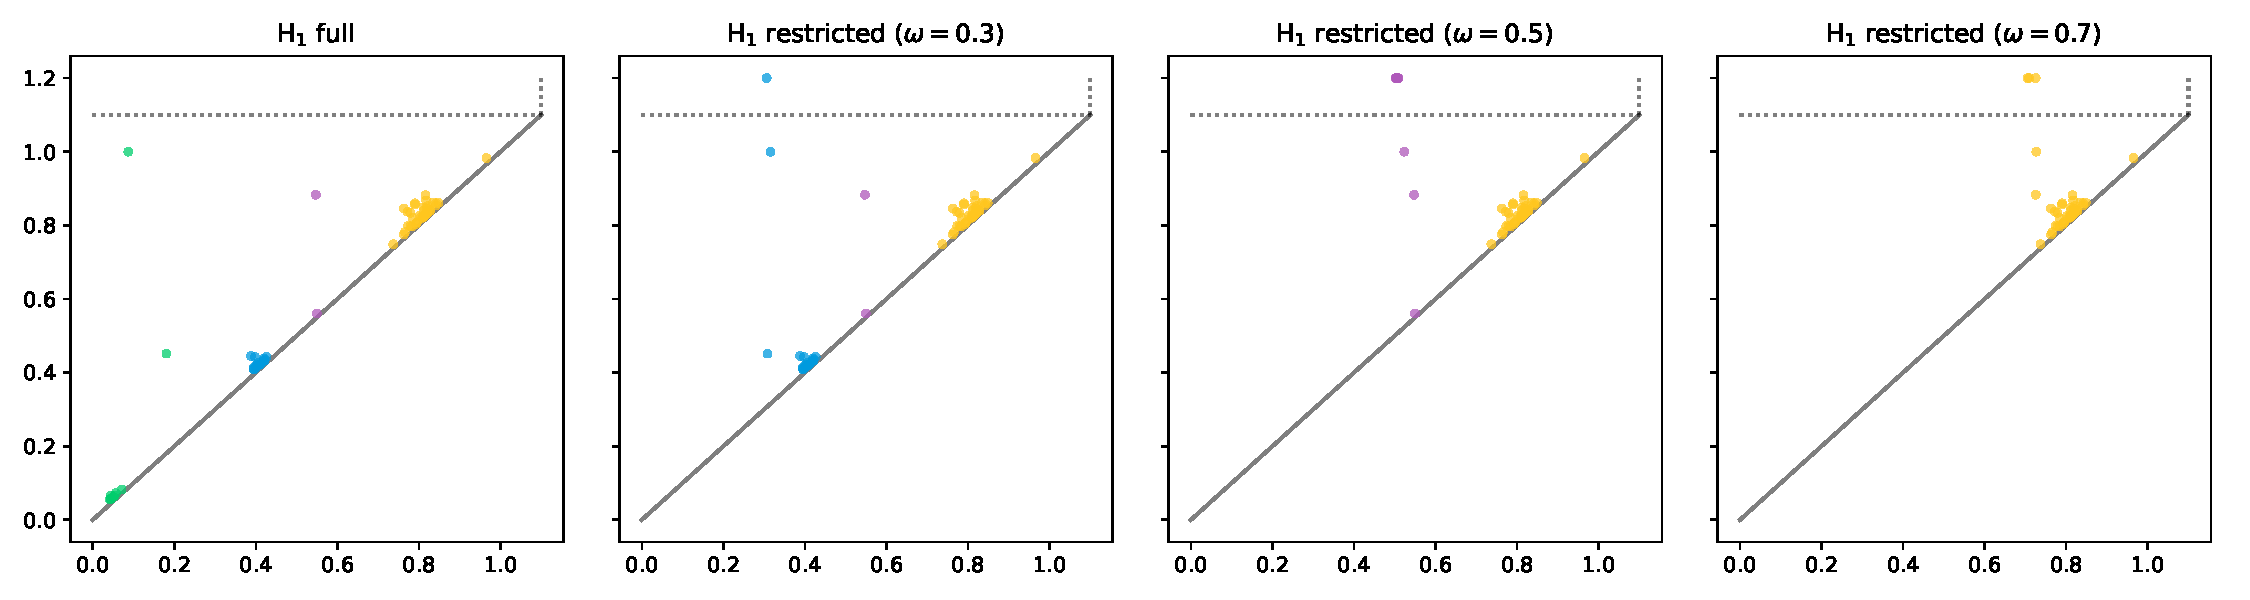
\includegraphics[trim=0 0 790 0, clip, width=0.3\textwidth]{figures/matching2/full-dgm.pdf}
  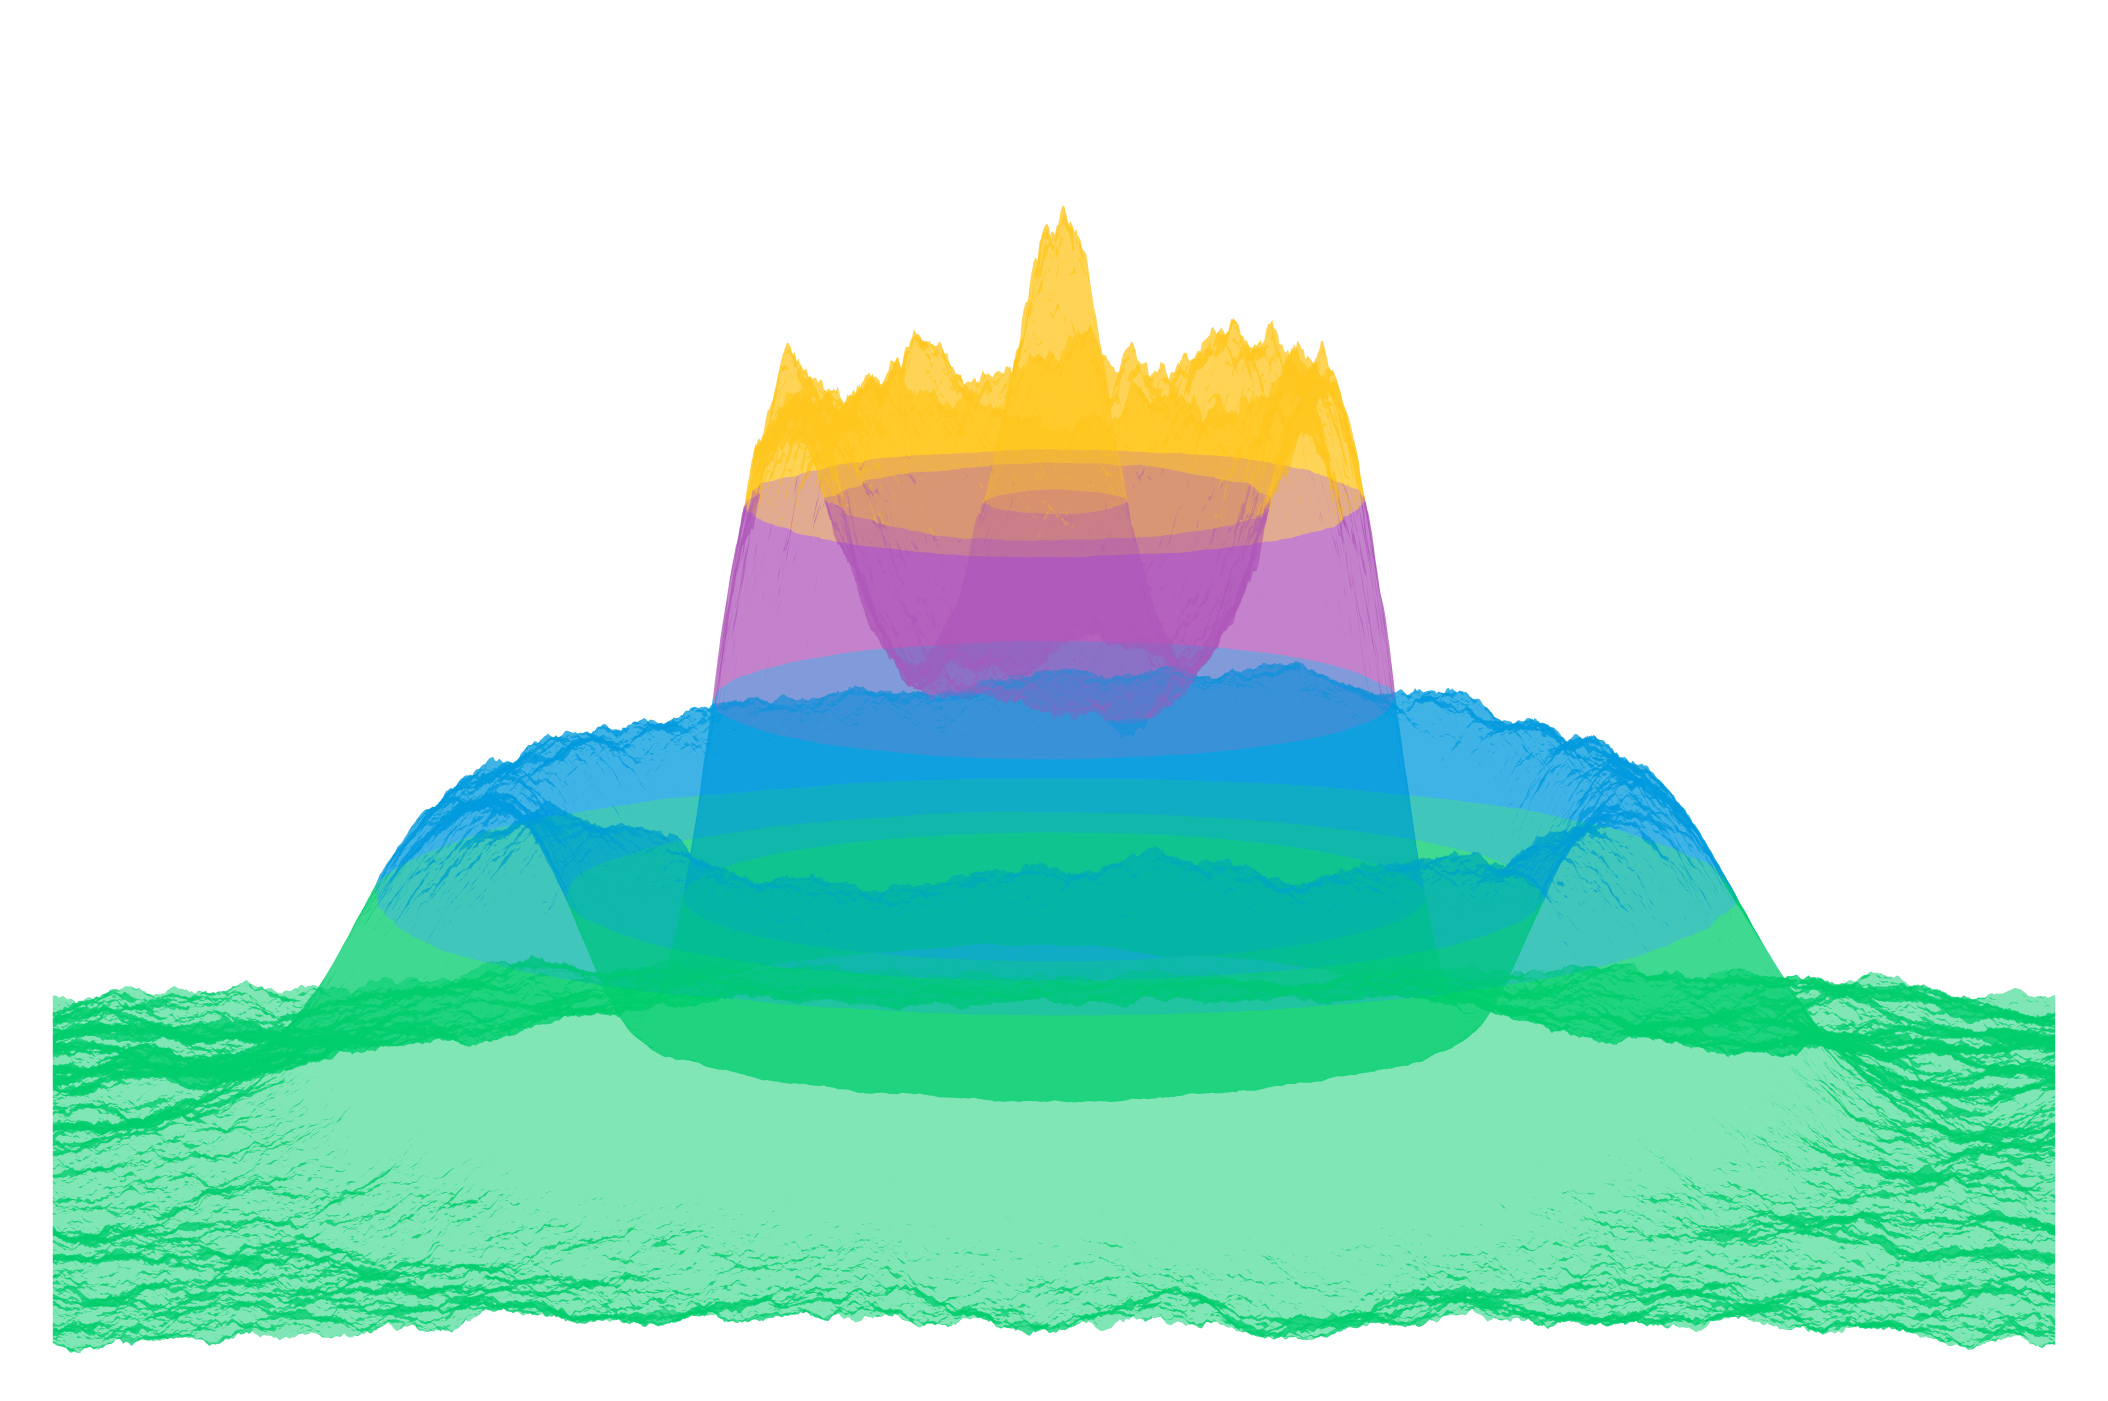
\includegraphics[trim=-350 -800 -700 -300, clip, width=0.4\textwidth]{figures/matching2/full-surf_side-lowres.png}
  
\includegraphics[trim=0 -800 0 0, width=0.25\textwidth]{figures/matching2/full-surf_top-lowres.png}
  % \includegraphics[trim=0 0 0 -10, clip, width=\textwidth]{scripts/figures/matching1/817_1024-3_1-1_1.png}
  \caption{The $\hom_1$ persistence diagram of the sinusoidal function pictured to the right.
  Features are colored by birth time, infinite features are drawn above the dotted line.}\label{fig:ripple1}
\end{figure}

Throughout, the four interlevel sets shown correspond to the ranges $[0, 0.3)$, $[0.3, 0.5)$, $[0.5, 0.7)$, and $[0.7, 1)$, respectively.
Our persistent homology computations were done primarily with Dionysus~\cite{morozov12dionysus} augmented with custom software for computing representative cycles of infinite features.
\footnote{3D figures were made with MayaVi, all other figures were made with Matplotlib.}
The persistent homology of our function was computed with the lower-star filtration of the Freudenthal triangulation on an $N\times N$ grid over $[-1,1]\times[-1,1]\subset\R^2$.
We take this filtration as $\{\rips^{2\delta}(P_\alpha)\}$ where $P$ is the set of grid points and $\delta = \sqrt{2} / N$.

We note that the purpose of these experiments is not to demonstrate the effectiveness of our approximation by Rips complexes, but to demonstrate the relationships between restricted, relative, and truncated diagrams.
Therefore, for simplicity, we will omit the inclusion $\rips^{2\delta}(P_\alpha)\hookrightarrow\rips^{4\delta}(P_\alpha)$ and take the persistent homology of $\{\rips^{2\delta}(P_\alpha)\}$ with sufficiently small $\delta$ as our ground-truth.
% However, in order to keep our diagrams clean we show only those features a distance at least $4\delta$ from the diagonal.
% Note that these features are \emph{not} removed from the diagram, and considered in all computations.

In the following we will take $N = 1024$, so $\delta\approx 1.4\times 10^{-3}$, as our ground-truth.
Figure~\ref{fig:ripple1} shows the \emph{full diagram} of our function with features colored by birth time.
Therefore, for $\omega = 0.3, 0.5, 0.7$ the \emph{truncated diagram} is obtained by successively removing features in each interlevel set.
Recall the \emph{restricted diagram} is that of the function restricted to the $\omega$ \emph{superlvel} set filtration, and computed with $\{\rips^{2\delta}(P_\alpha\setminus Q_\omega)\}$.
We will compare this restricted diagram with the \emph{relative diagram}, computed as the relative persistent homology of the filtration of pairs $\{\rips^{2\delta}(P_\alpha, Q_\omega)\}$.

\paragraph*{The issue with restricted diagrams.}

% In order to get an initial sense of the difference between relative and restricted diagrams we first compare the bottleneck distance of each to the truncated diagram.
% As we have shown the relative diagram is equal to the truncated diagram with additional infinite features we will remove all infinite features from the bottleneck computation.
% We therefore expect the distance between the relative and truncated diagrams to be zero for $N=1024$.

Figure~\ref{fig:bottleneck} shows the bottleneck distance from the truncated diagram at full resolution ($N = 1024$) to both the relative and restricted diagrams with varying resolution.
Specifically, the function on a $1024\times 1024$ grid is down-sampled to grids ranging from $64\times 64$ to $1024\times 1024$.
We also show the expected bottleneck distance to the true truncated diagram given by the interleaving in Theorem~\ref{thm:interleaving_main_2} in black.

\begin{figure}[htbp]
  \centering
  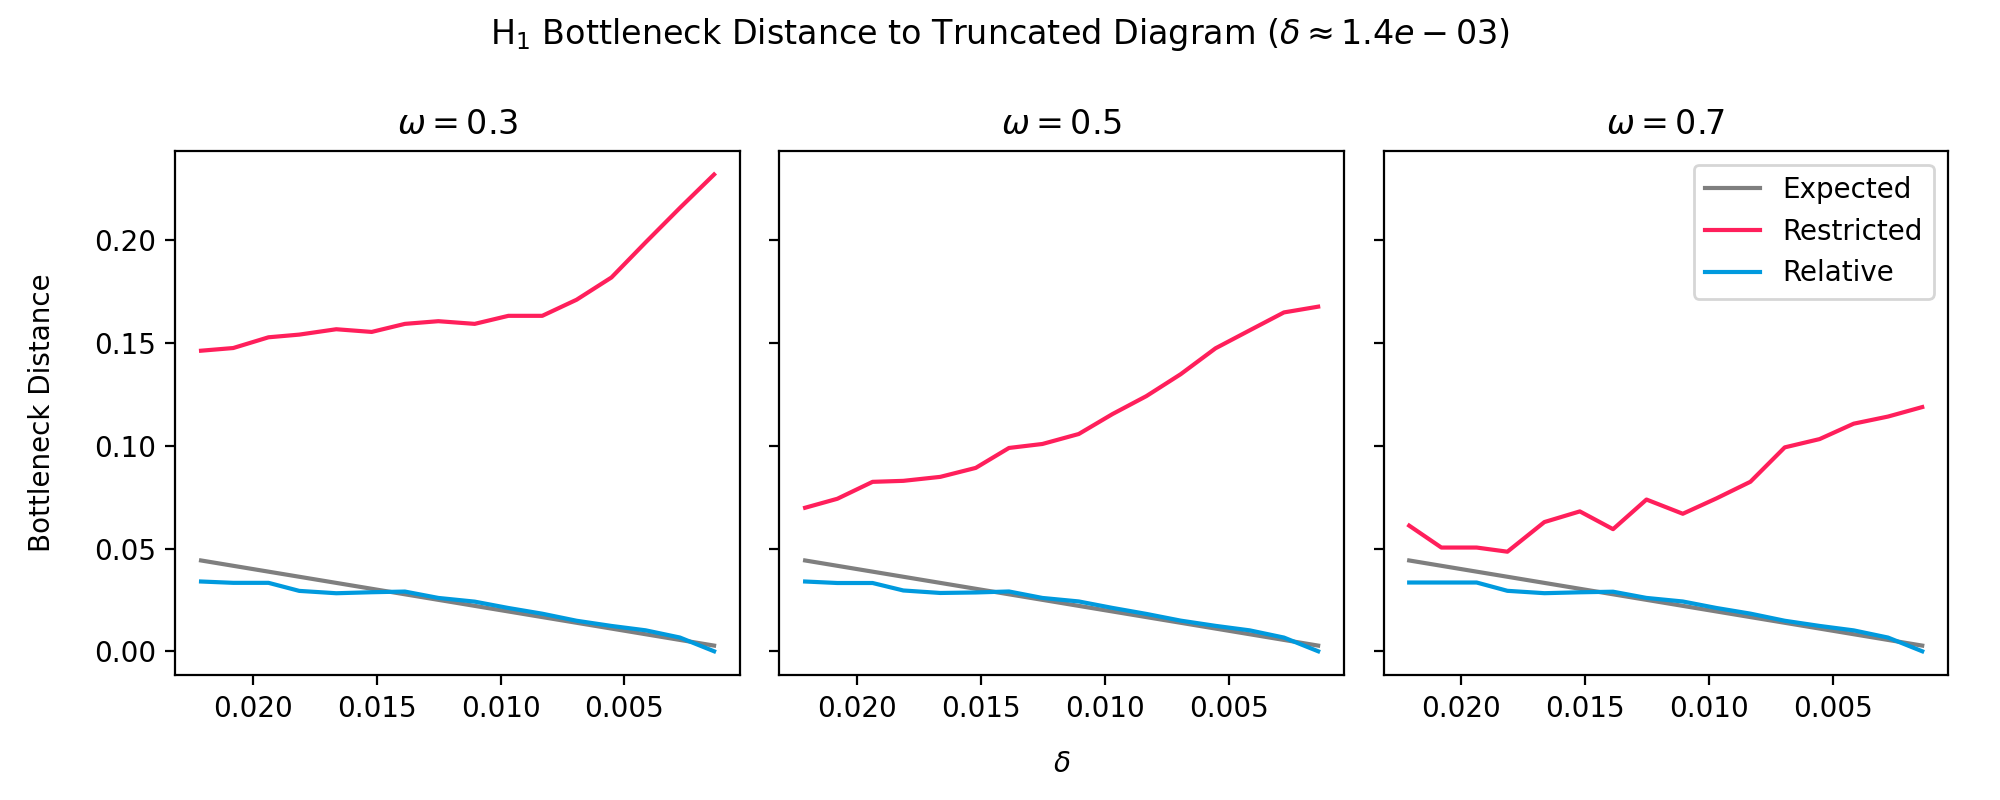
\includegraphics[width=0.95\textwidth]{figures/matching2/bottleneck_delta.png}
  \caption{Comparison of the bottleneck distance between the truncated diagram and those of the restricted and relative diagrams with increasing resolution.}\label{fig:bottleneck}
\end{figure}

As we can see, the relative diagram clearly performs better than the restricted diagram, which diverges with increasing resolution.
% The reason for this is shown in Figure~\ref{fig:restricted} which depicts the restricted diagrams at $\omega = 0.3, 0.5,$ and $0.7$ at full resolution.
Recall that 1-dimensional features that are born before $\omega$ and die after $\omega$ become infinite 2-dimensional features in the relative diagram, with birth time equal to the death time of the corresponding feature in the full diagram.
These same features remain 1-dimensional figures in the restricted diagram, but with their birth times shifted to $\omega$.
% Indeed, the resulting restricted diagram may be closer to the full diagram for sufficiently small $\omega$.
% However, the distance will be proportional to the difference between $\omega$ and the true birth time.

\begin{figure}[htbp]
  \centering
  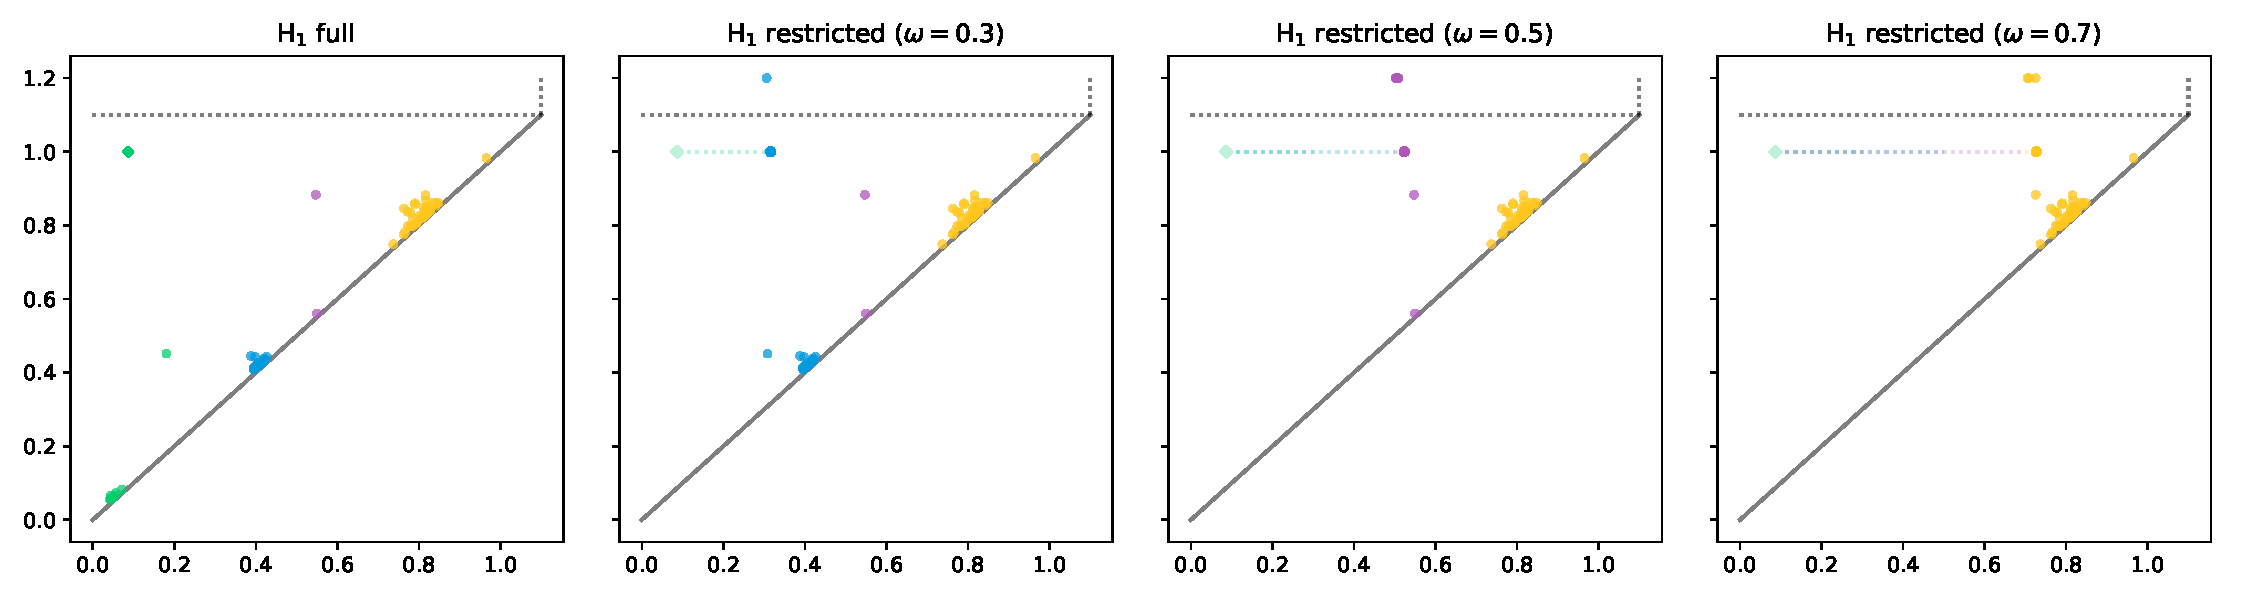
\includegraphics[trim=0 0 -10 0, clip, width=\textwidth]{figures/matching2/dgm-1.pdf}
  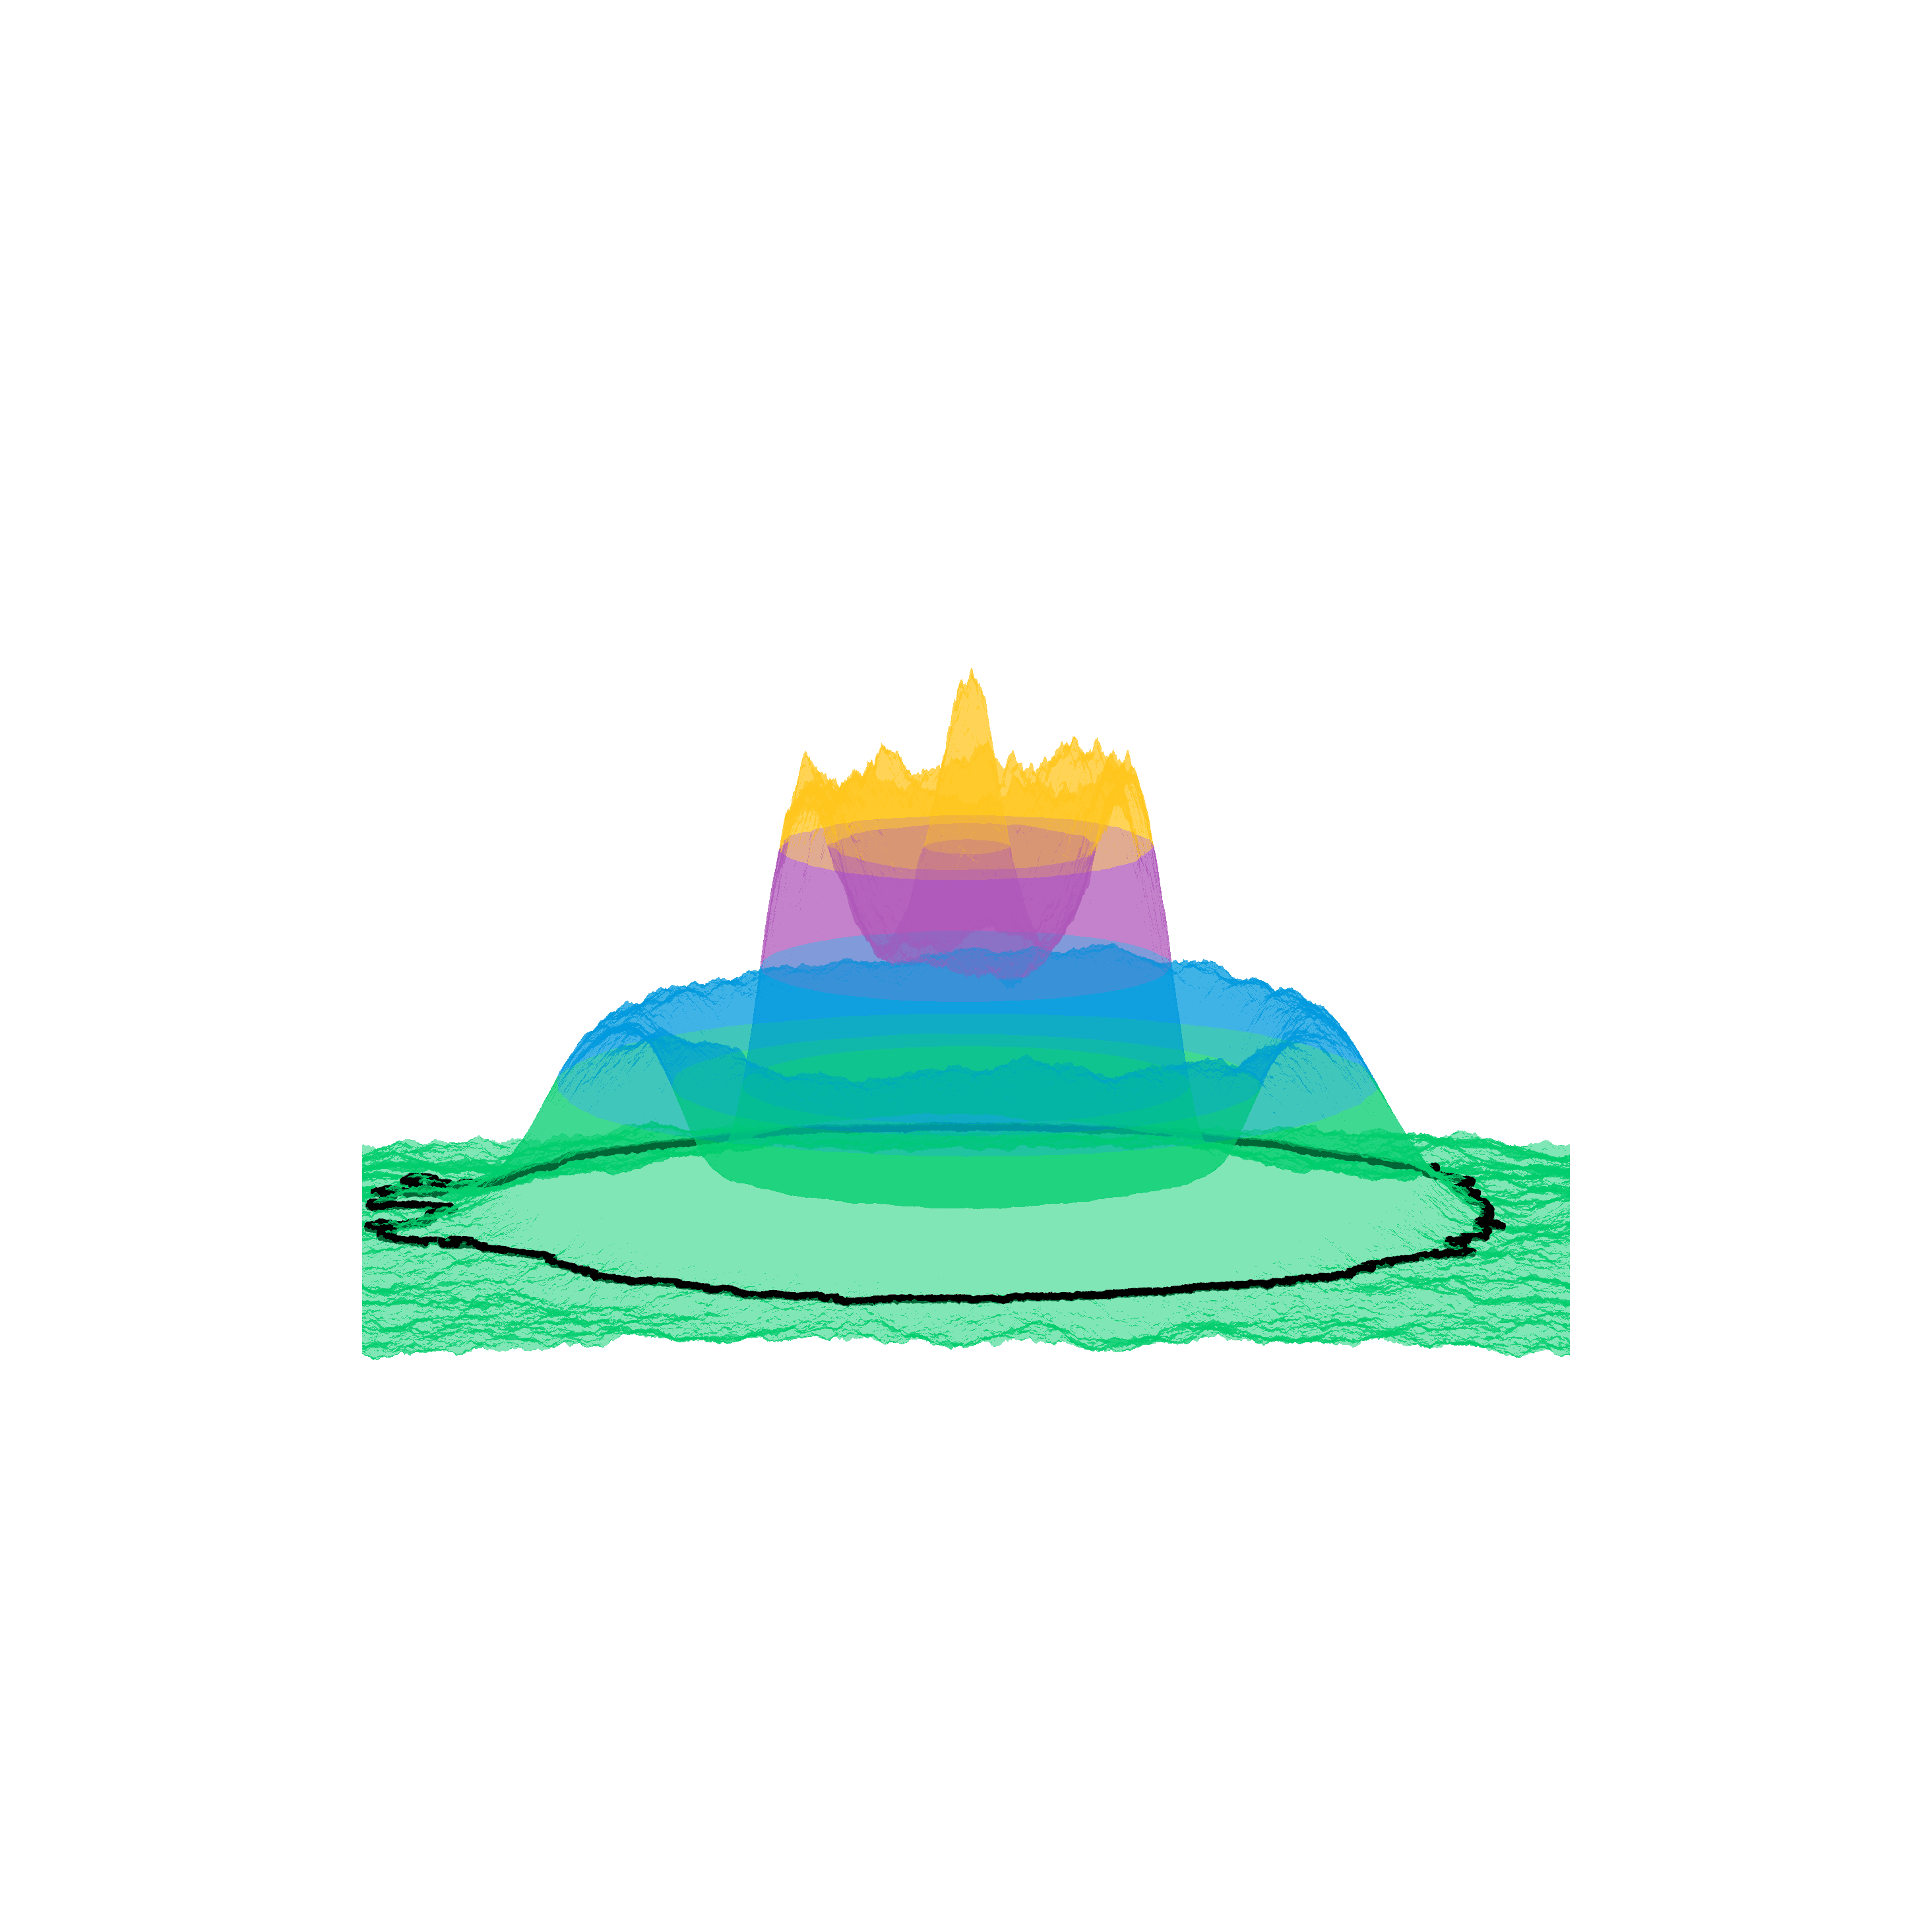
\includegraphics[trim=500 800 500 800, clip, width=0.24\textwidth]{figures/matching2/surf_side-1.png}
  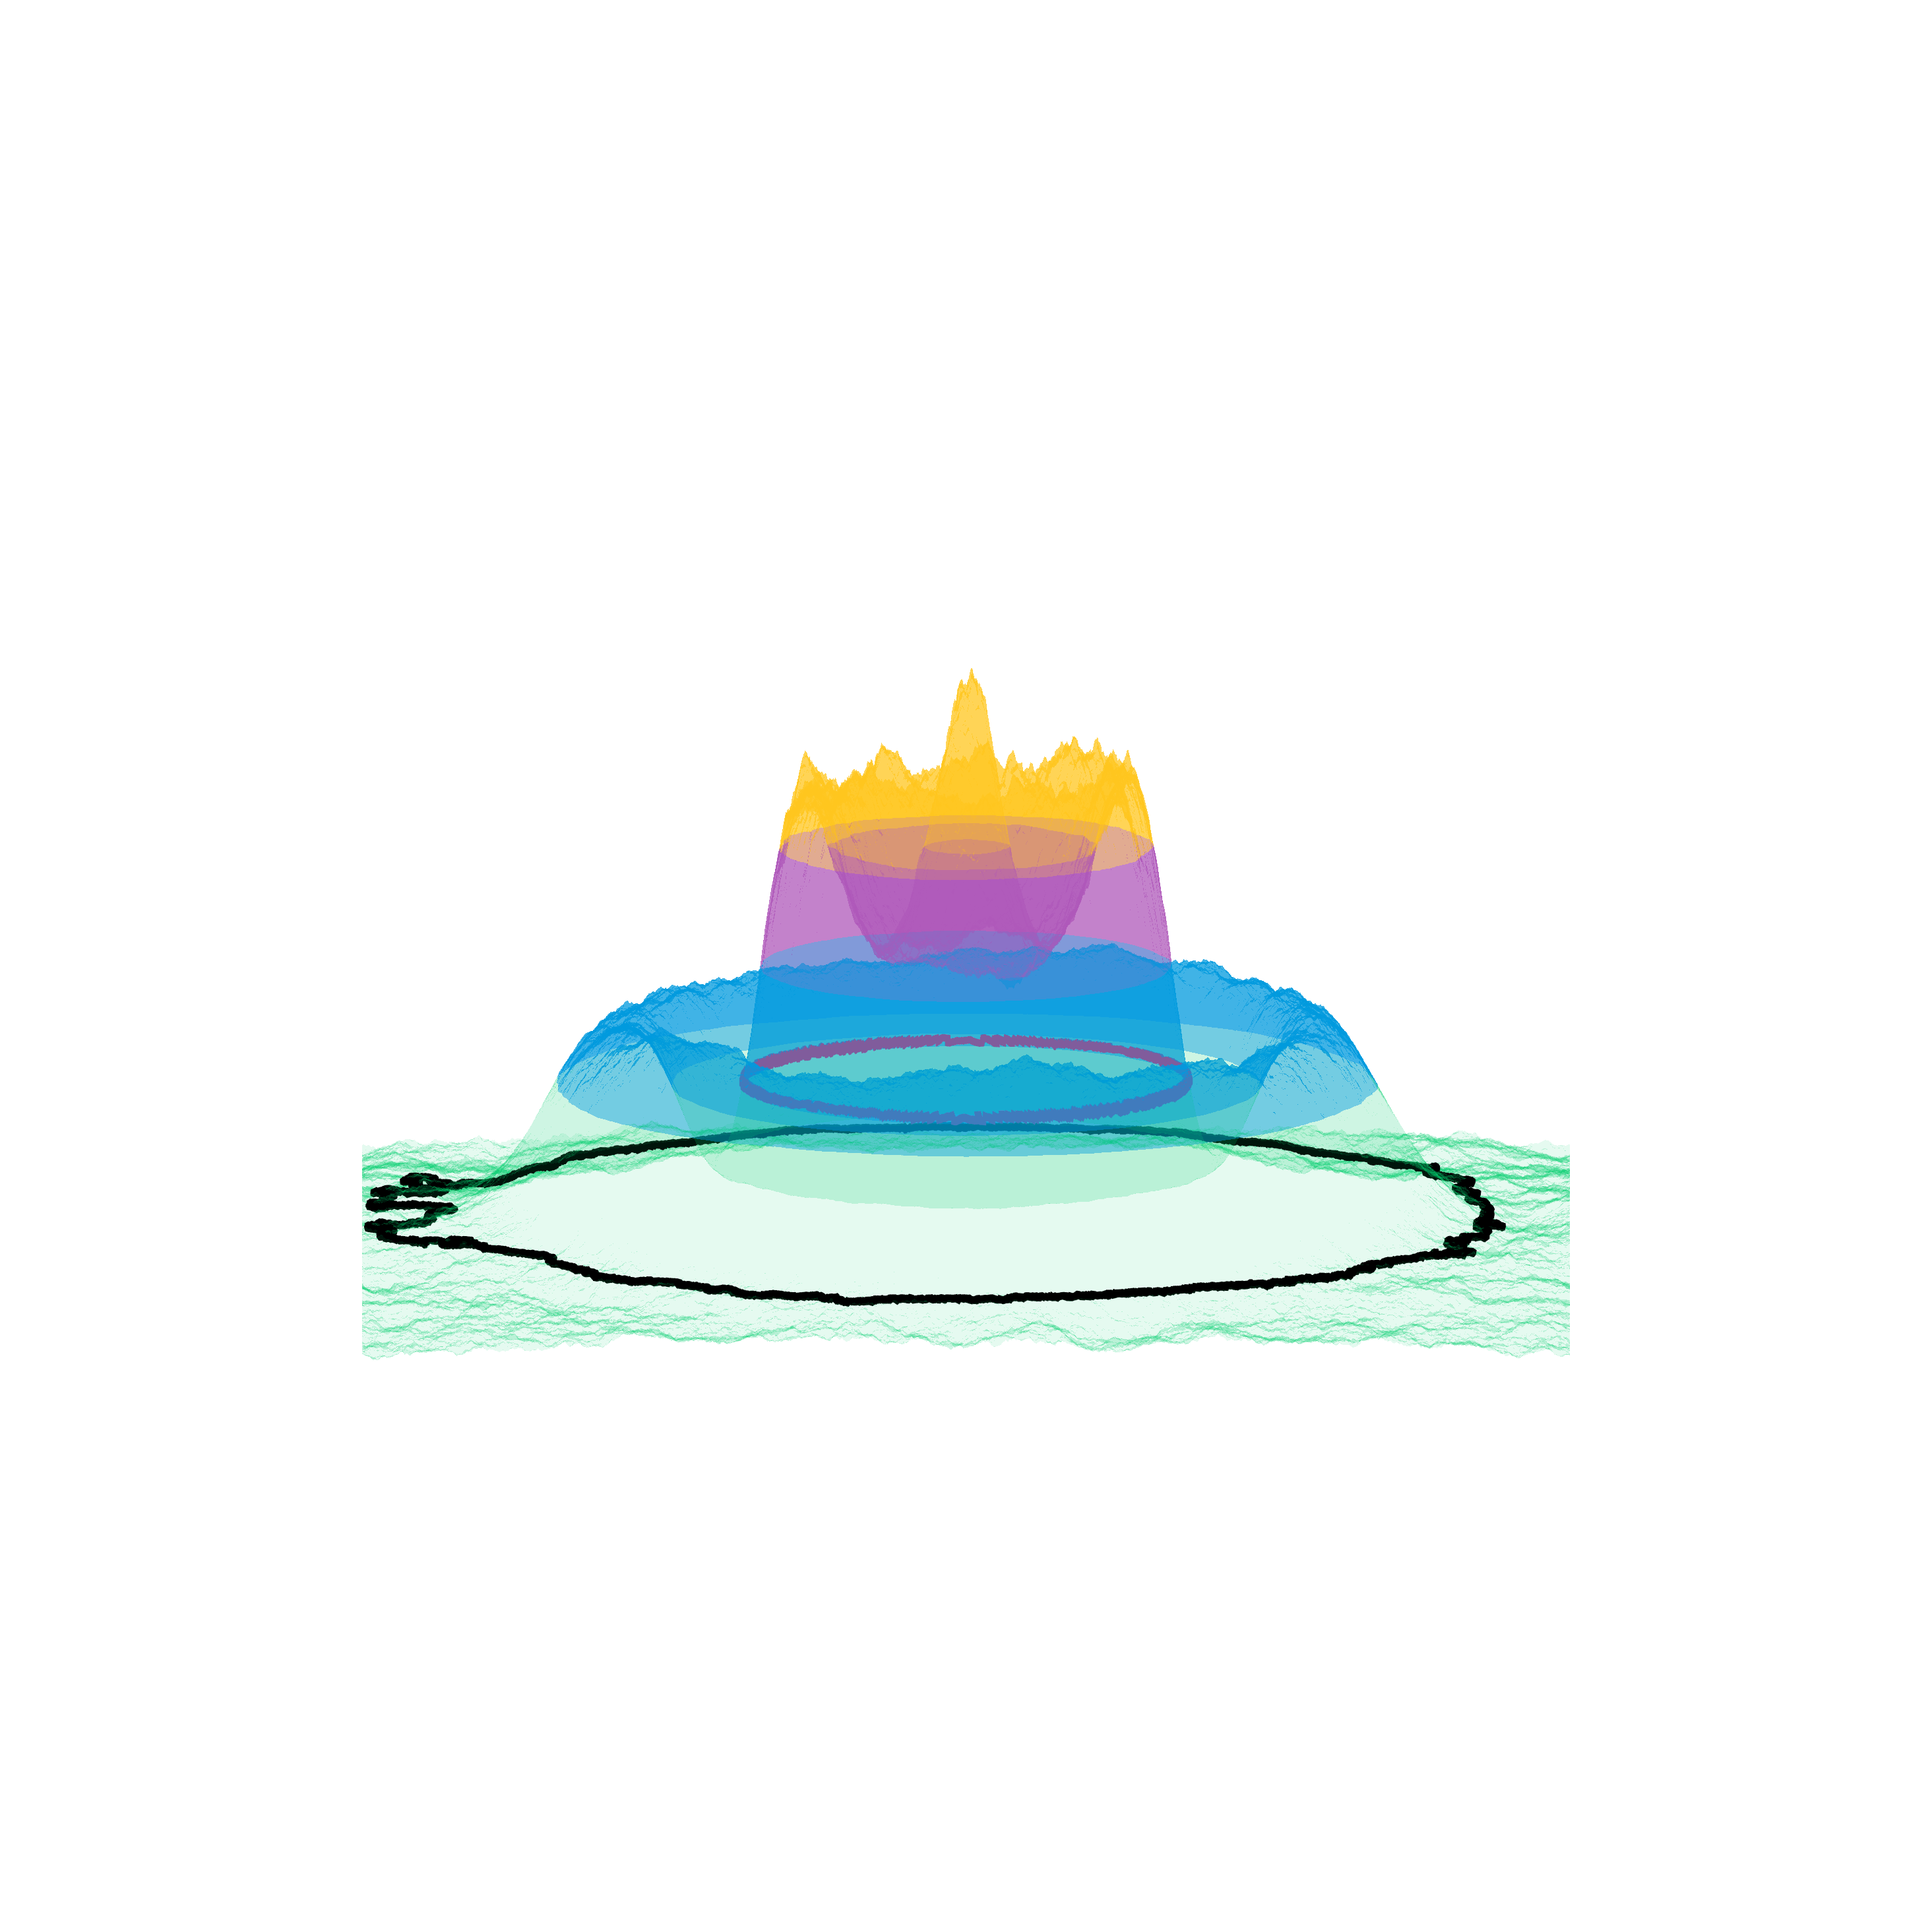
\includegraphics[trim=500 800 500 800, clip, width=0.24\textwidth]{figures/matching2/surf_side-1_0.png}
  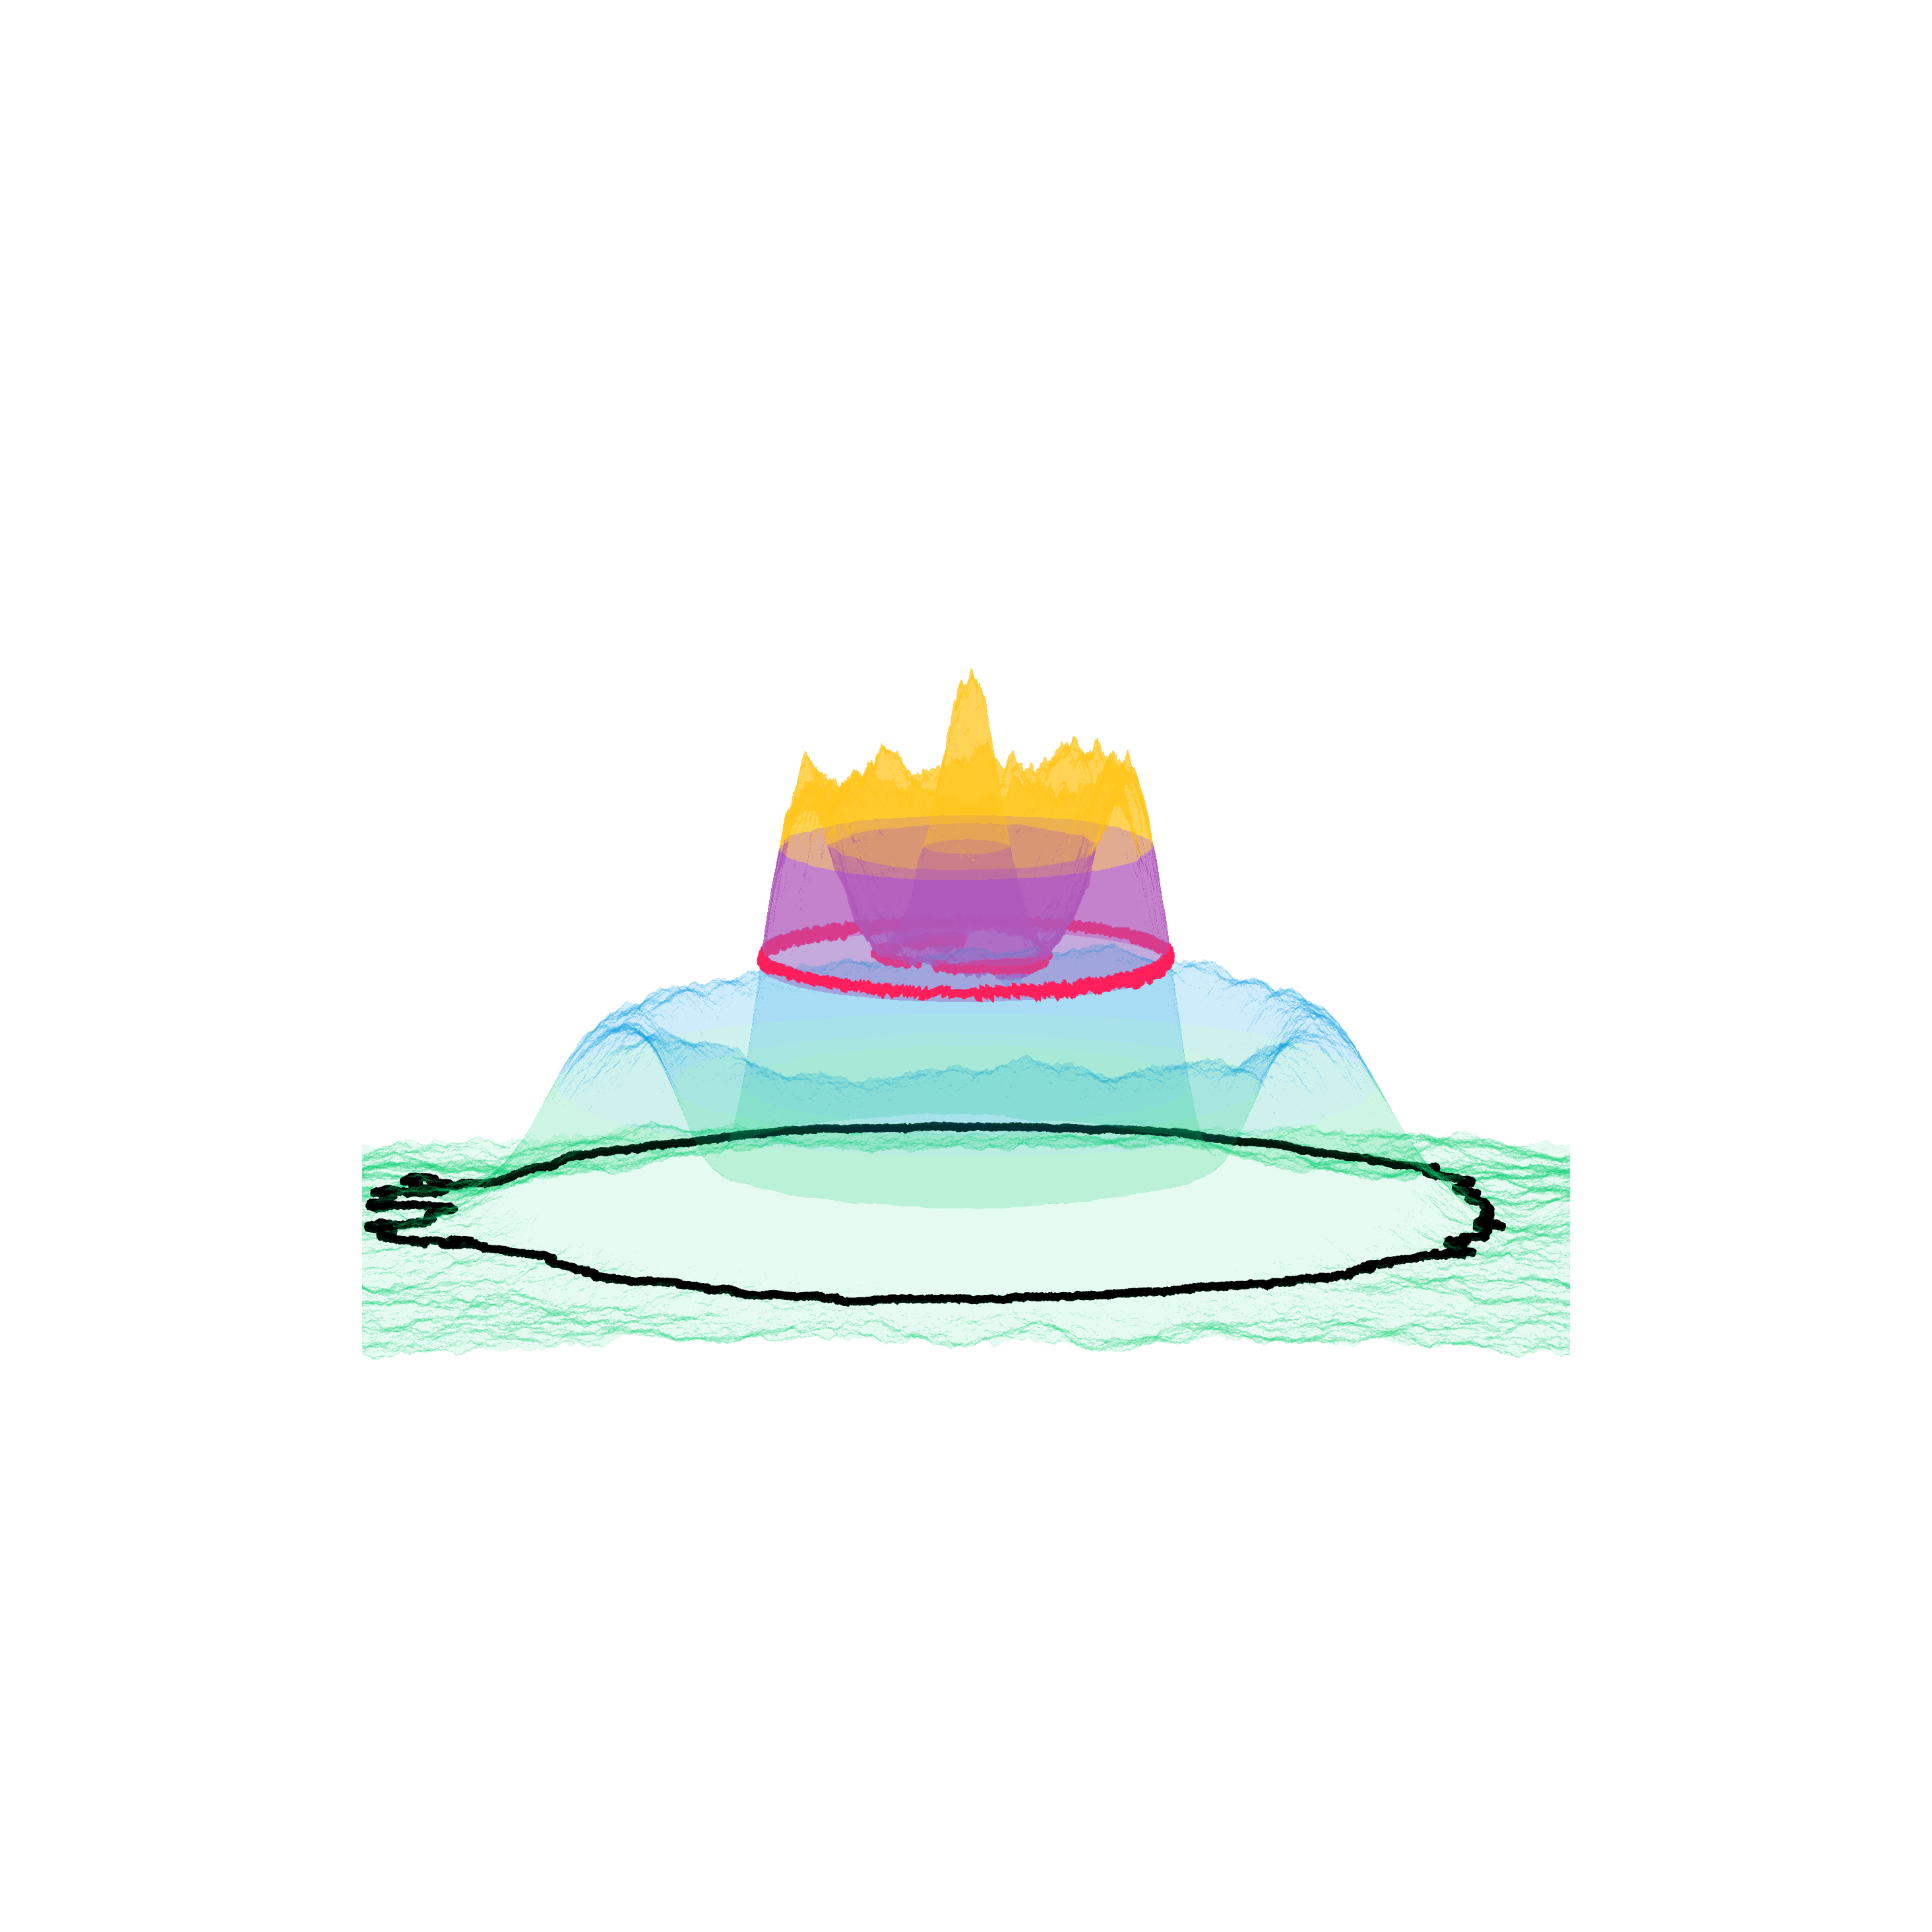
\includegraphics[trim=500 800 500 800, clip, width=0.24\textwidth]{figures/matching2/surf_side-1_1.png}
  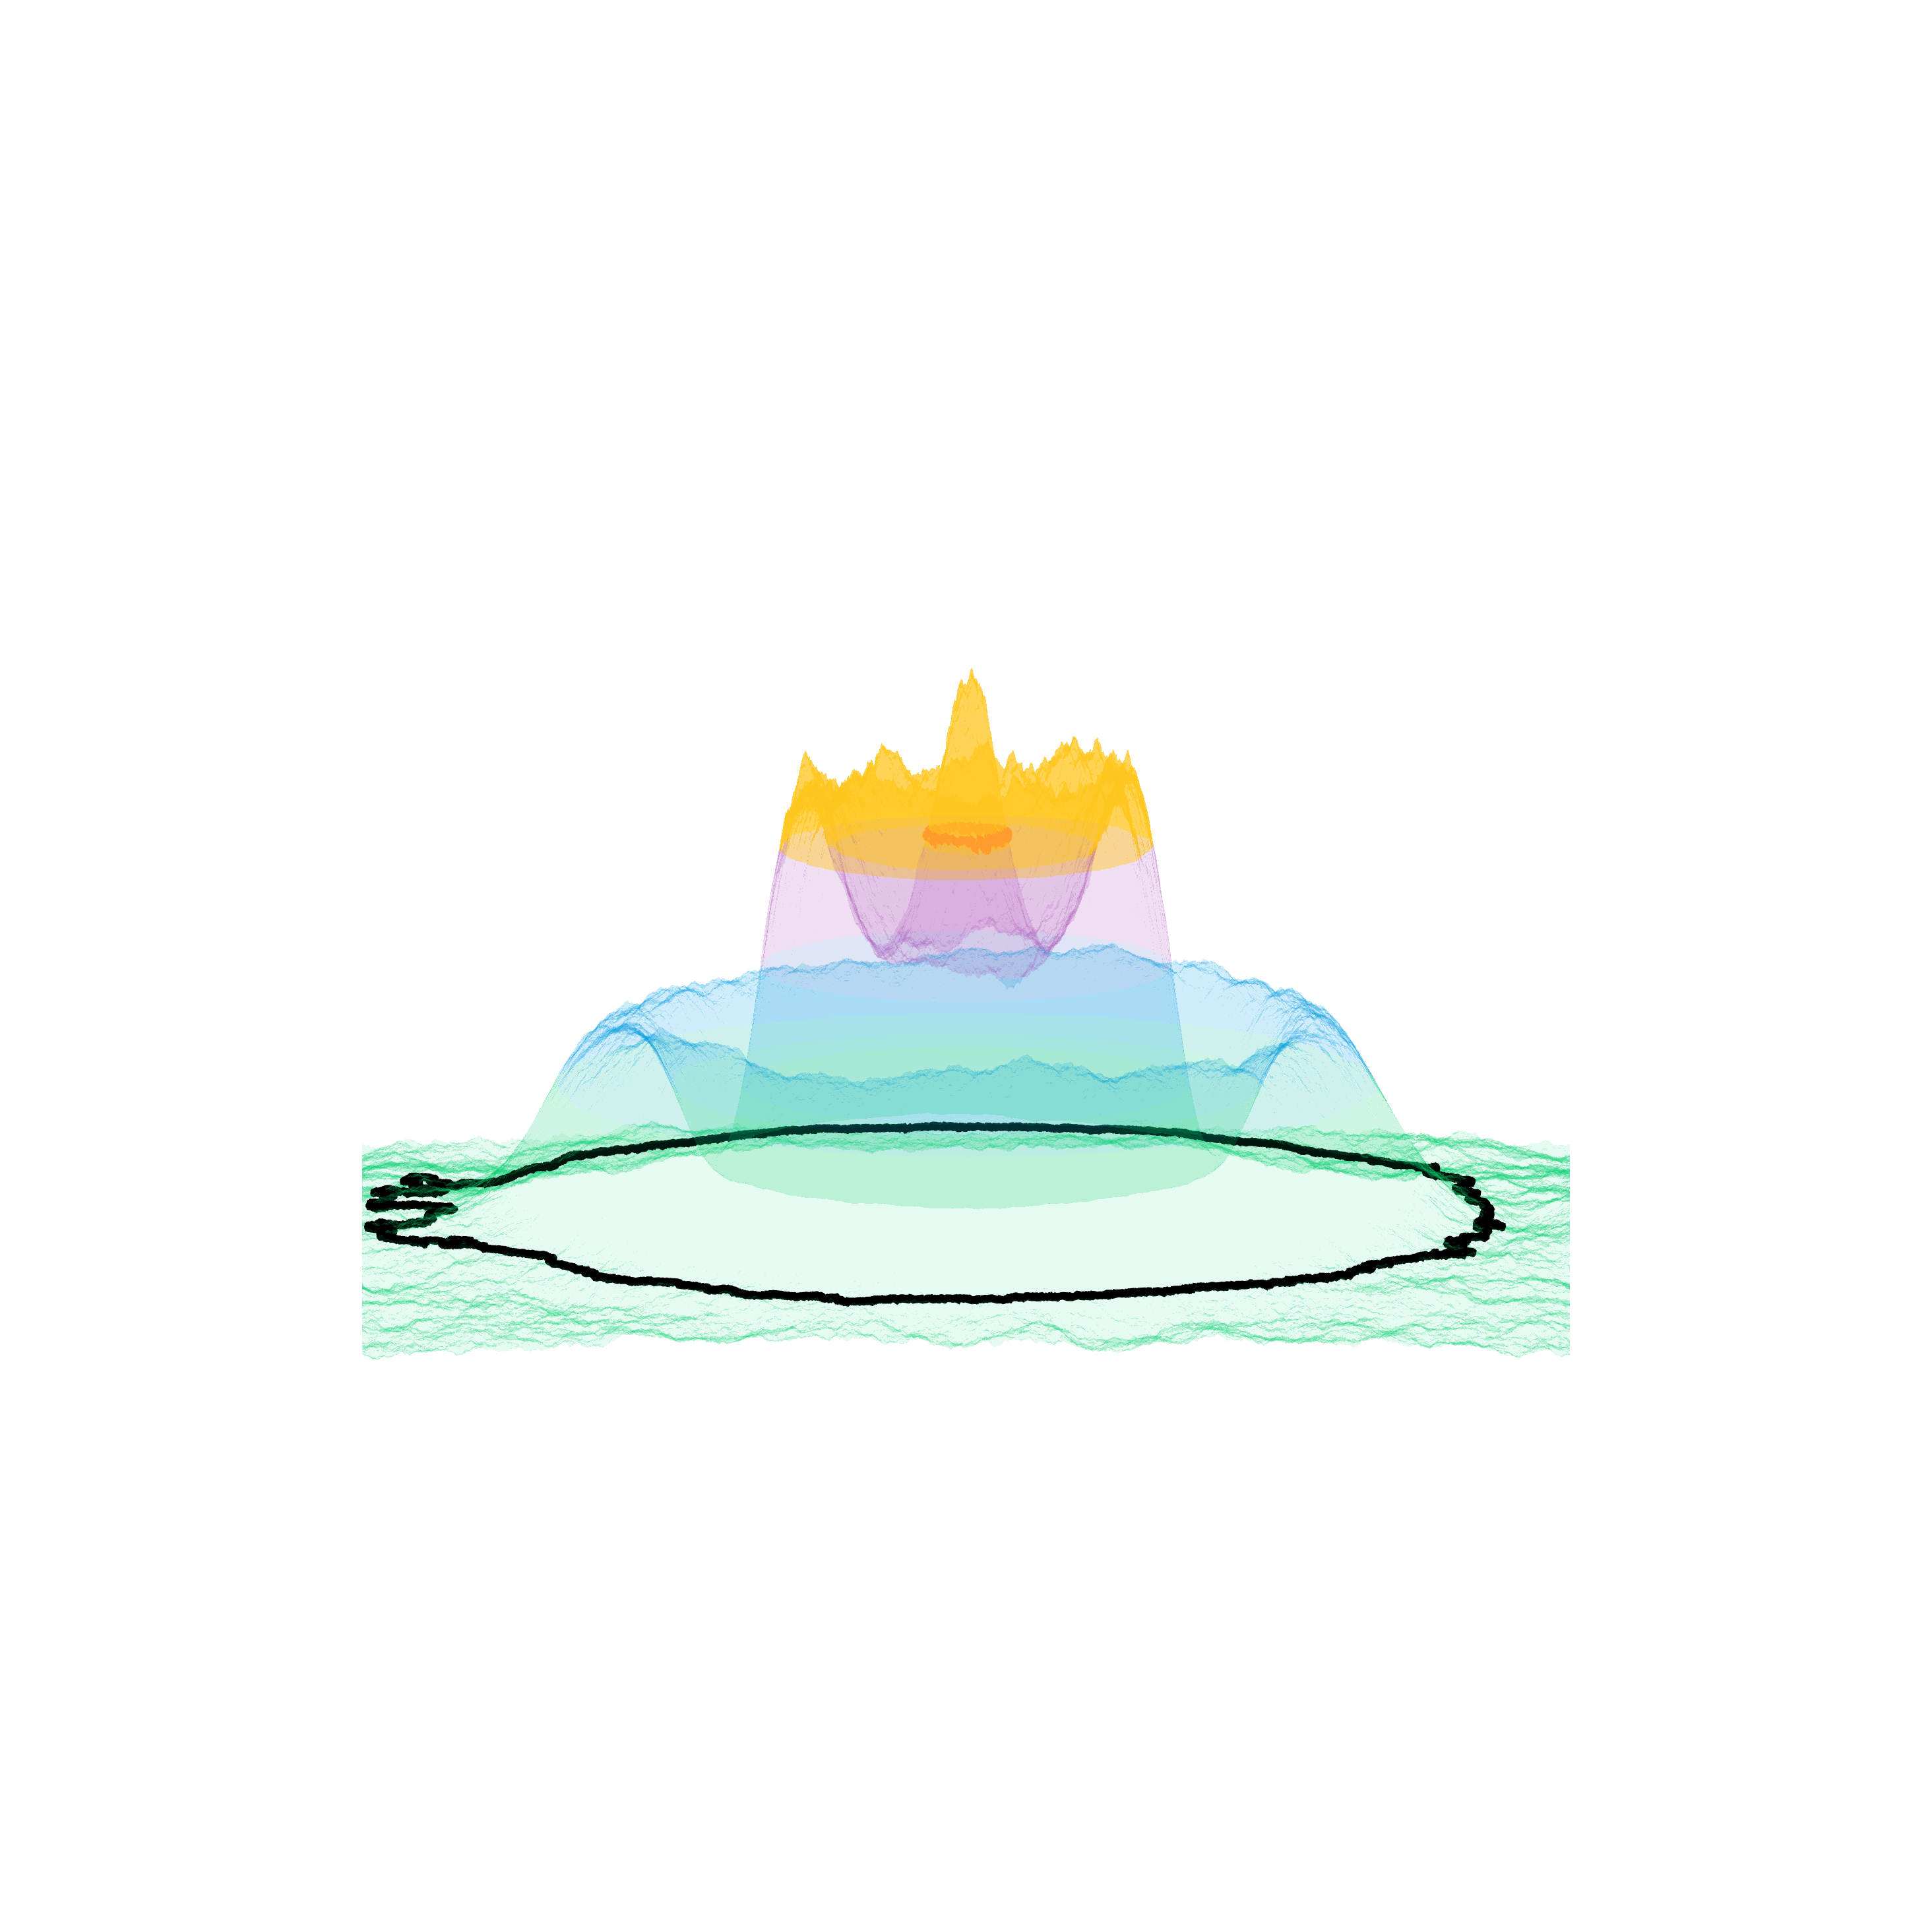
\includegraphics[trim=500 800 500 800, clip, width=0.24\textwidth]{figures/matching2/surf_side-1_2.png}
  
\includegraphics[trim=500 500 500 500, clip, width=0.24\textwidth]{figures/matching2/surf_top-1.png}
  
\includegraphics[trim=500 500 500 500, clip, width=0.24\textwidth]{figures/matching2/surf_top-1_0.png}
  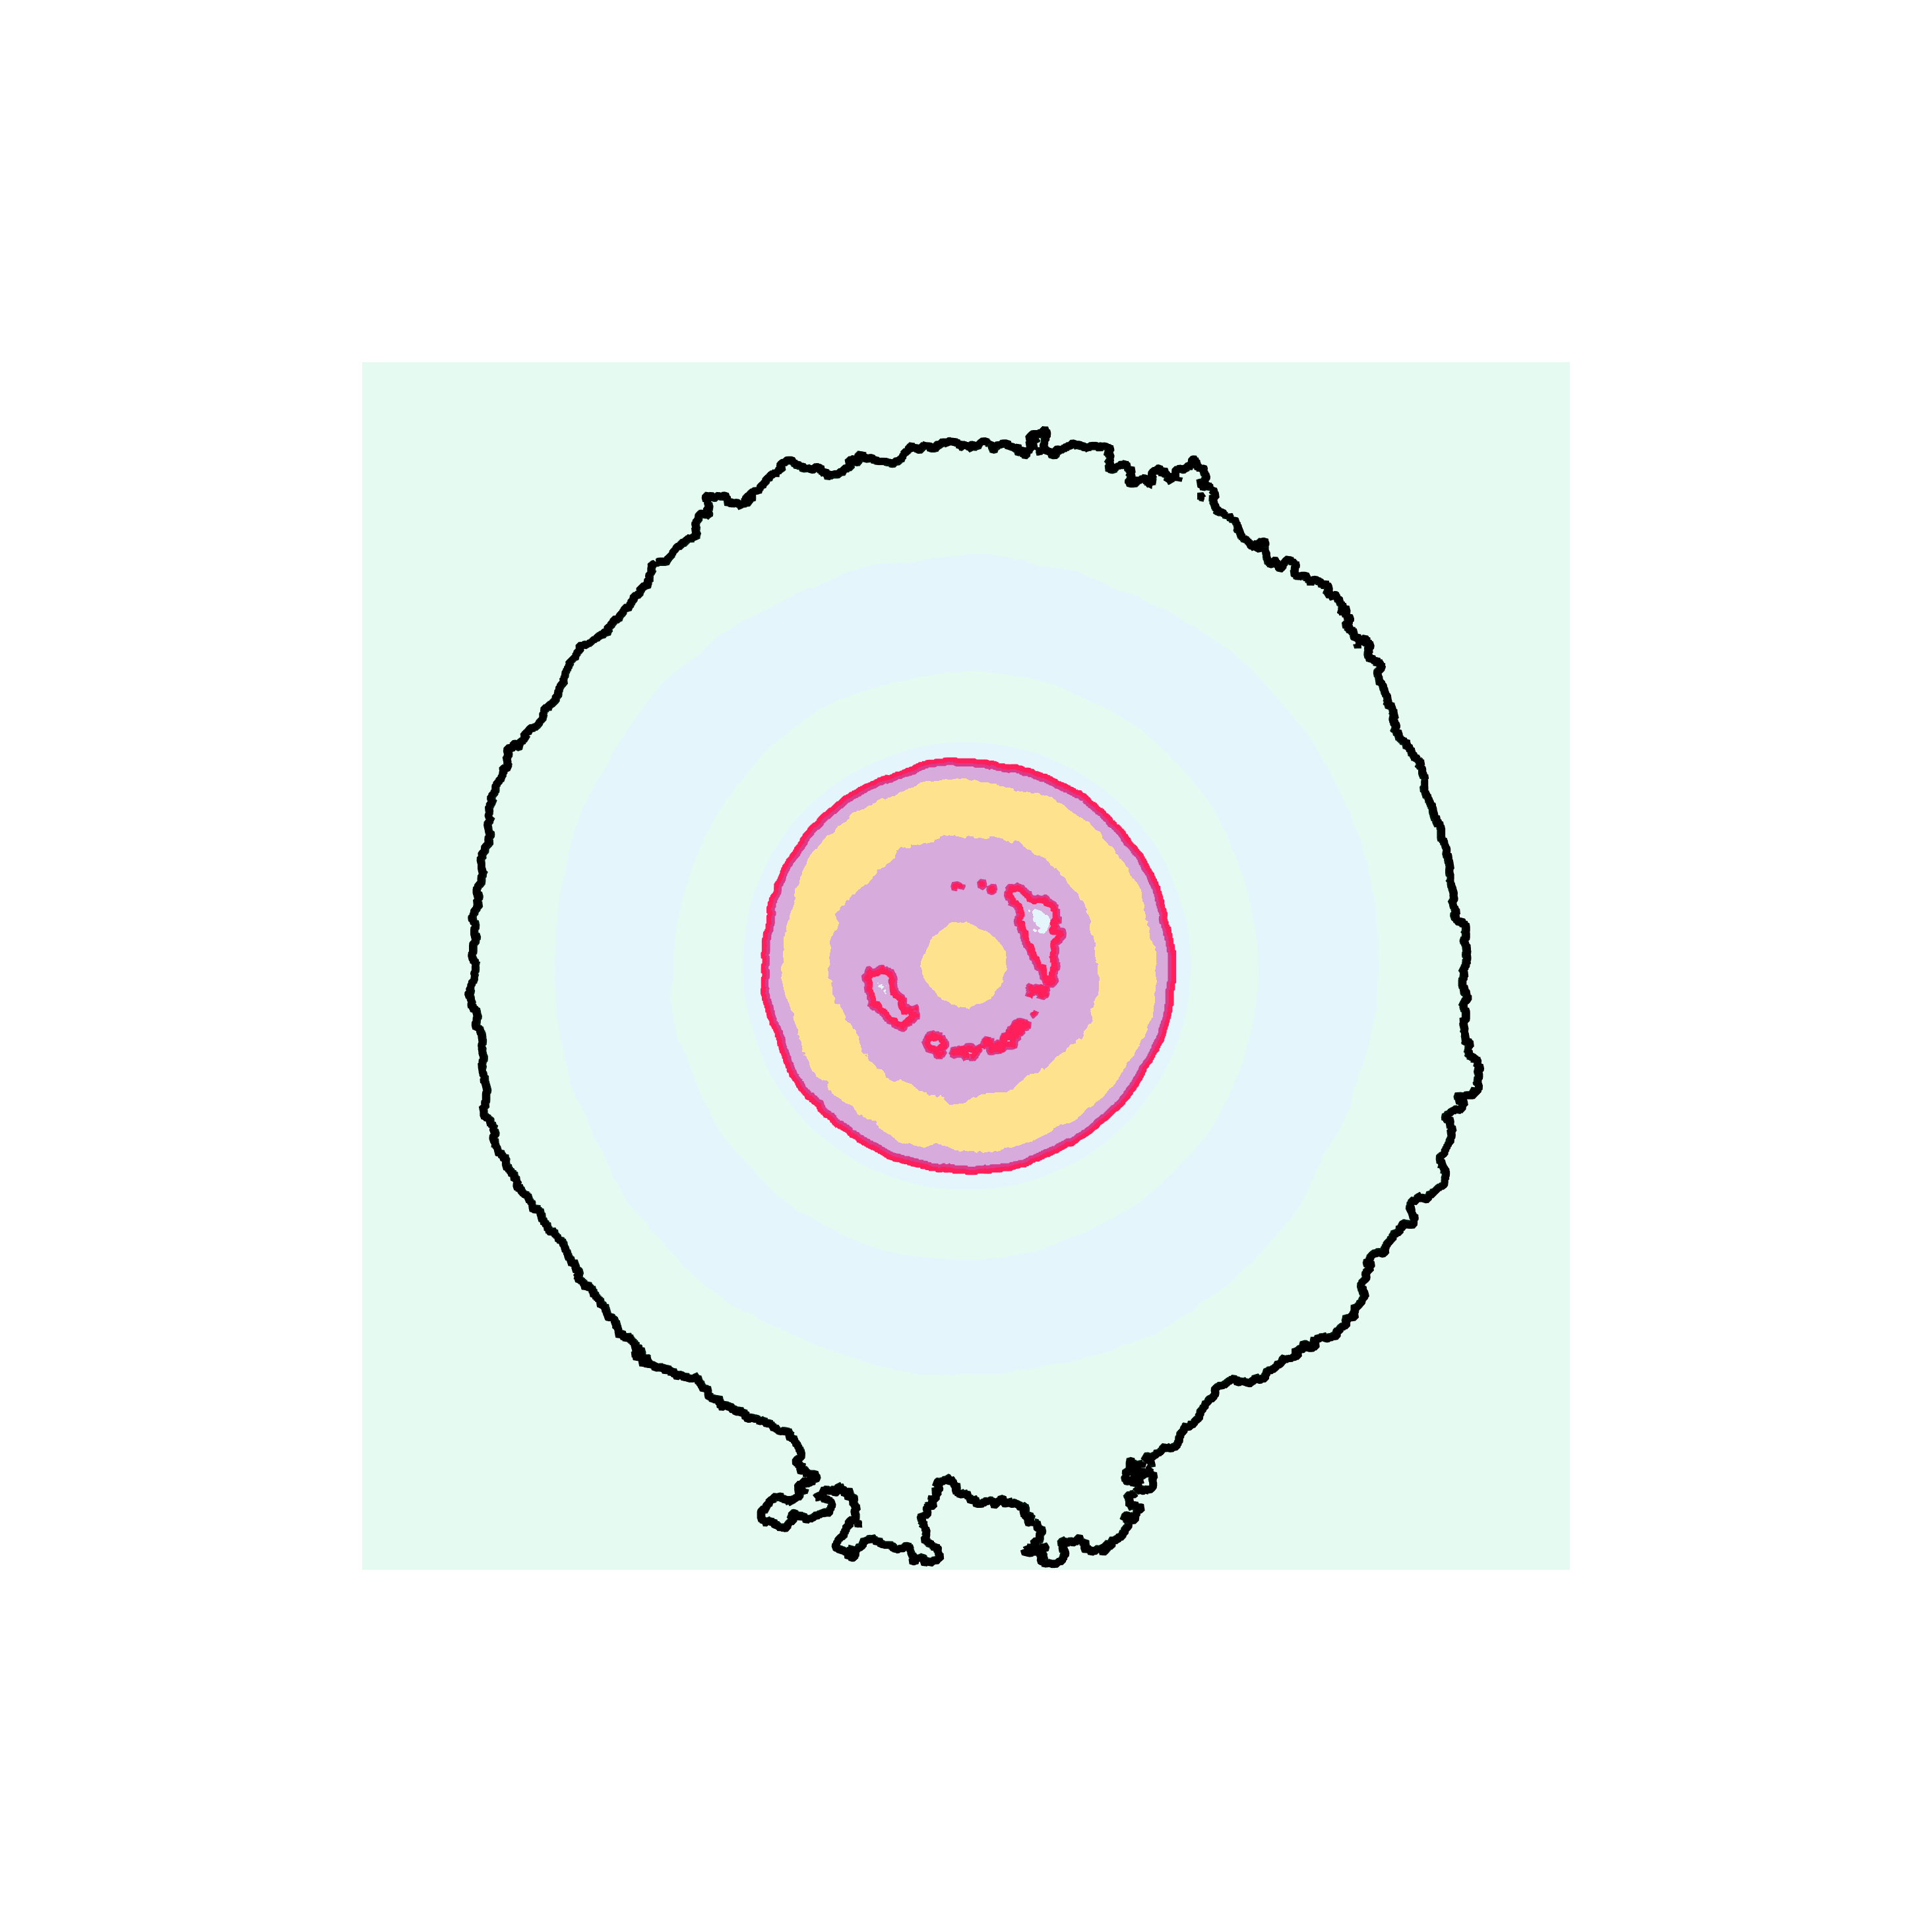
\includegraphics[trim=500 500 500 500, clip, width=0.24\textwidth]{figures/matching2/surf_top-1_1.png}
  
\includegraphics[trim=500 500 500 500, clip, width=0.24\textwidth]{figures/matching2/surf_top-1_2.png}
  \caption{(Top) $\hom_1$ persistence diagrams of the function depicted in Figure~\ref{fig:ripple1} restricted to \emph{superlevel} sets at $\omega = 0.3, 0.5,$ and $0.7$ (on a $1024\times 1024$ grid).
  The matching is shown between a feature in the full diagram (marked with a diamond) with its representative cycle in black.
  The corresponding representative cycle in the restricted diagram is pictured in red.}\label{fig:restricted}
\end{figure}

Figure~\ref{fig:restricted} shows this distance for a feature that persists throughout the diagram.
As the restricted diagram in full resolution the restricted filtration is a subset of the full filtration, so these features can be matched by their death simplices.
For illustrative purposes we also show the representative cycles associated with these features.

% We imagine a setting where we would like to classify a function using a sample that cannot be verified below some known $\omega$.
% That is, we can only check for coverage of the super-levelset $D\setminus B_\omega$ using the variation of the TCC we have introduced in the previous sections.
% We would then like to classify the function with the bottleneck distance to a set of known functions based on the region we cover.
% However, as we have shown, the restricted diagram may contain artifacts of features born before $\omega$ which will skew our measurement.
% Instead, as $\omega$ is known, we can compare the \emph{relative} diagram the collection of \emph{truncated} diagrams of known functions to get a better classification.

\paragraph*{Relative diagrams and reconstruction.}

\begin{figure}[htbp]
  \centering
  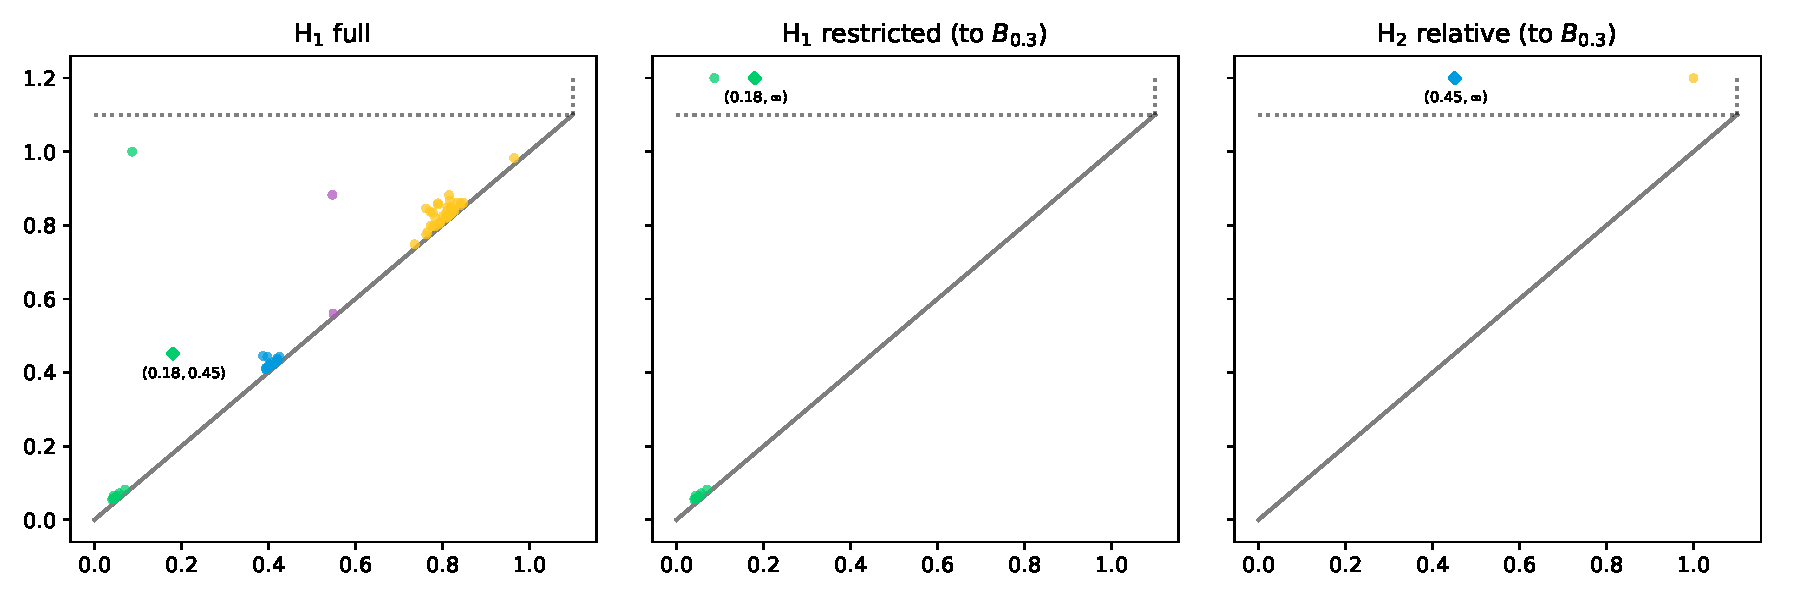
\includegraphics[width=0.9\textwidth]{figures/relative/dgm-0_0.pdf}
  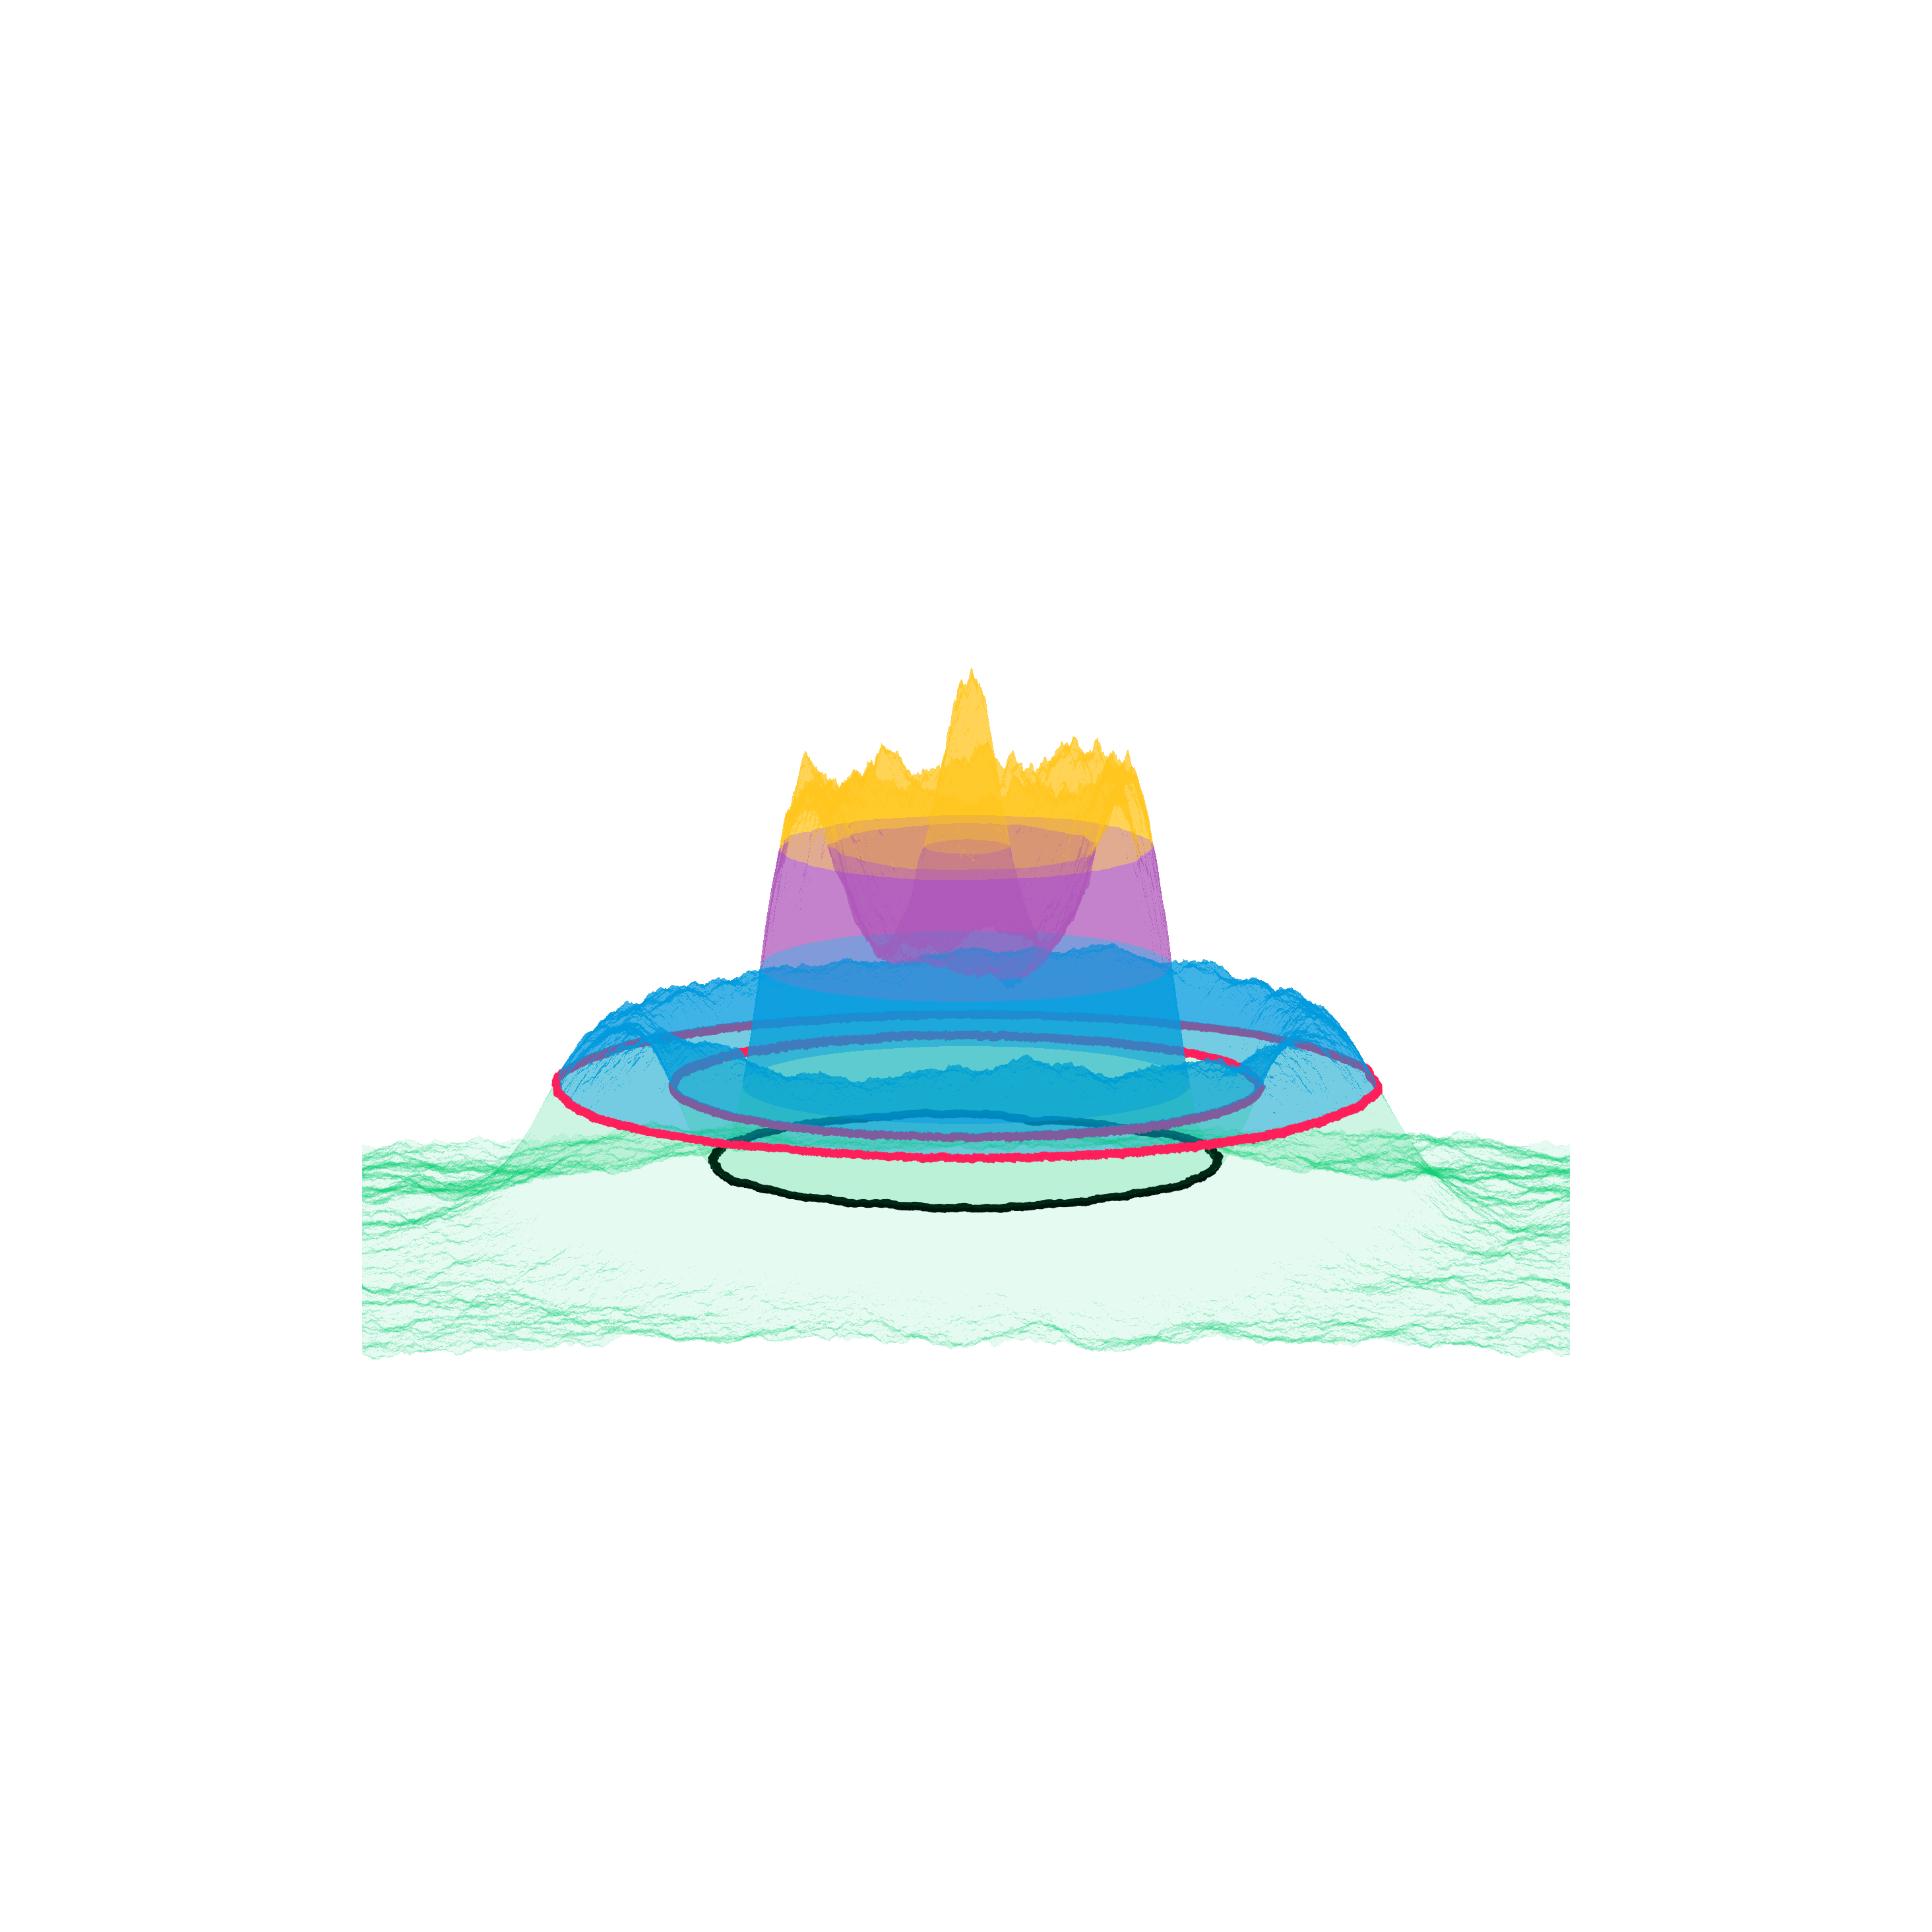
\includegraphics[trim=500 800 500 800, clip, width=0.35\textwidth]{figures/relative/surf_side-0_0.png}
  
\includegraphics[trim=500 500 500 500, clip, width=0.25\textwidth]{figures/relative/surf_top-0_0.png}
  % \caption{(Left) Full $\hom_1$ persistence diagram, (middle) $\hom_1$ persistence diagram of the function restricted to the \emph{sub}-levelset $B_{0.3}$, (right) $\hom_2$ persistence diagram of the the function realtive to the sub-levelset $B_{0.3}$.
  \caption{(Top) The indicated infinite features in the restricted and relative diagrams correspond to the birth and death of the 1-feature $(0.18, 0.45)$ in the full diagram.
  (Bottom) In black, the representative cycle of the infinite 1-feature born at 0.18 in the restricted diagram is shown in black.
  In red, the \emph{boundary} of the representative \emph{relative} 2-cycle born at 0.45 in the relative diagram is shown in red.}\label{fig:relative1}
\end{figure}

Now, imagine we obtain the persistence diagram of our sublevel set $B_\omega$.
That is, we now know that we cover $B_\omega$, or some subset, and do not want to re-compute the diagram above $\omega$.
If we compute the persistence diagram of the function restricted to the \emph{sublevel} set $B_\omega$ any 1-dimensional features born before $\omega$ that die after $\omega$ will remain infinite features in this restricted (below) diagram.
Indeed, we could match these infinite 1-features with the corresponding shifted finite 1-features in the restricted (above) diagram, as shown in Figure~\ref{fig:restricted}.
However, that would require sorting through all finite features that are born near $\omega$ and deciding if they are in fact features of the full diagram that have been shifted.

Recalling that these same features become infinite 2-features in the relative diagram, we can use the relative diagram instead and match infinite 1-features of the diagram restricted below to infinite 2-features in the relative diagram, as shown in Figures~\ref{fig:relative1} and~\ref{fig:relative2}.
For this example the sequence of birth times of relative 2-features in \emph{decreasing} order correspond to the deaths of restricted 1-features in \emph{increasing} order.
How to construct this matching in general, especially in the presence of infinite features in the full diagram, is the subject of future research.

\begin{figure}[htbp]
  \centering
  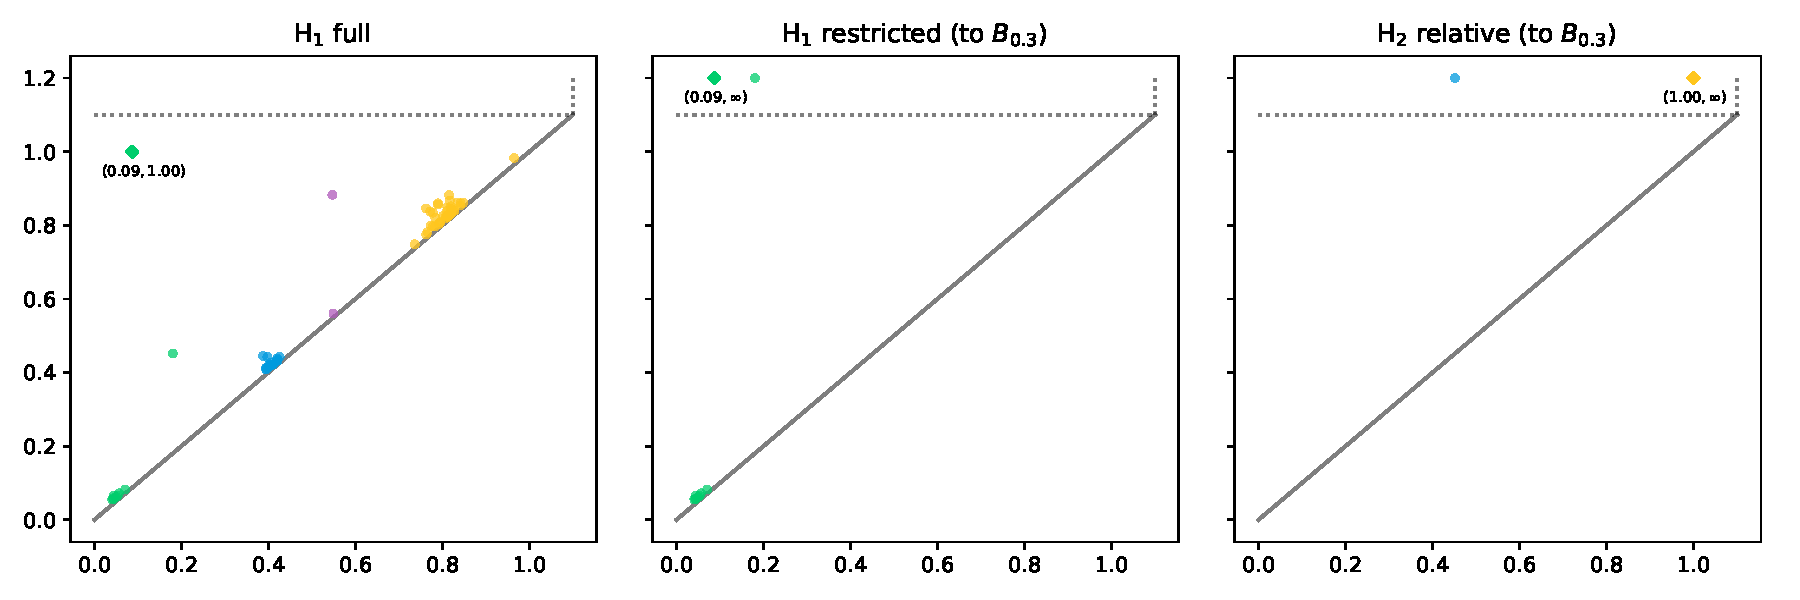
\includegraphics[width=0.9\textwidth]{figures/relative/dgm-0_1.pdf}
  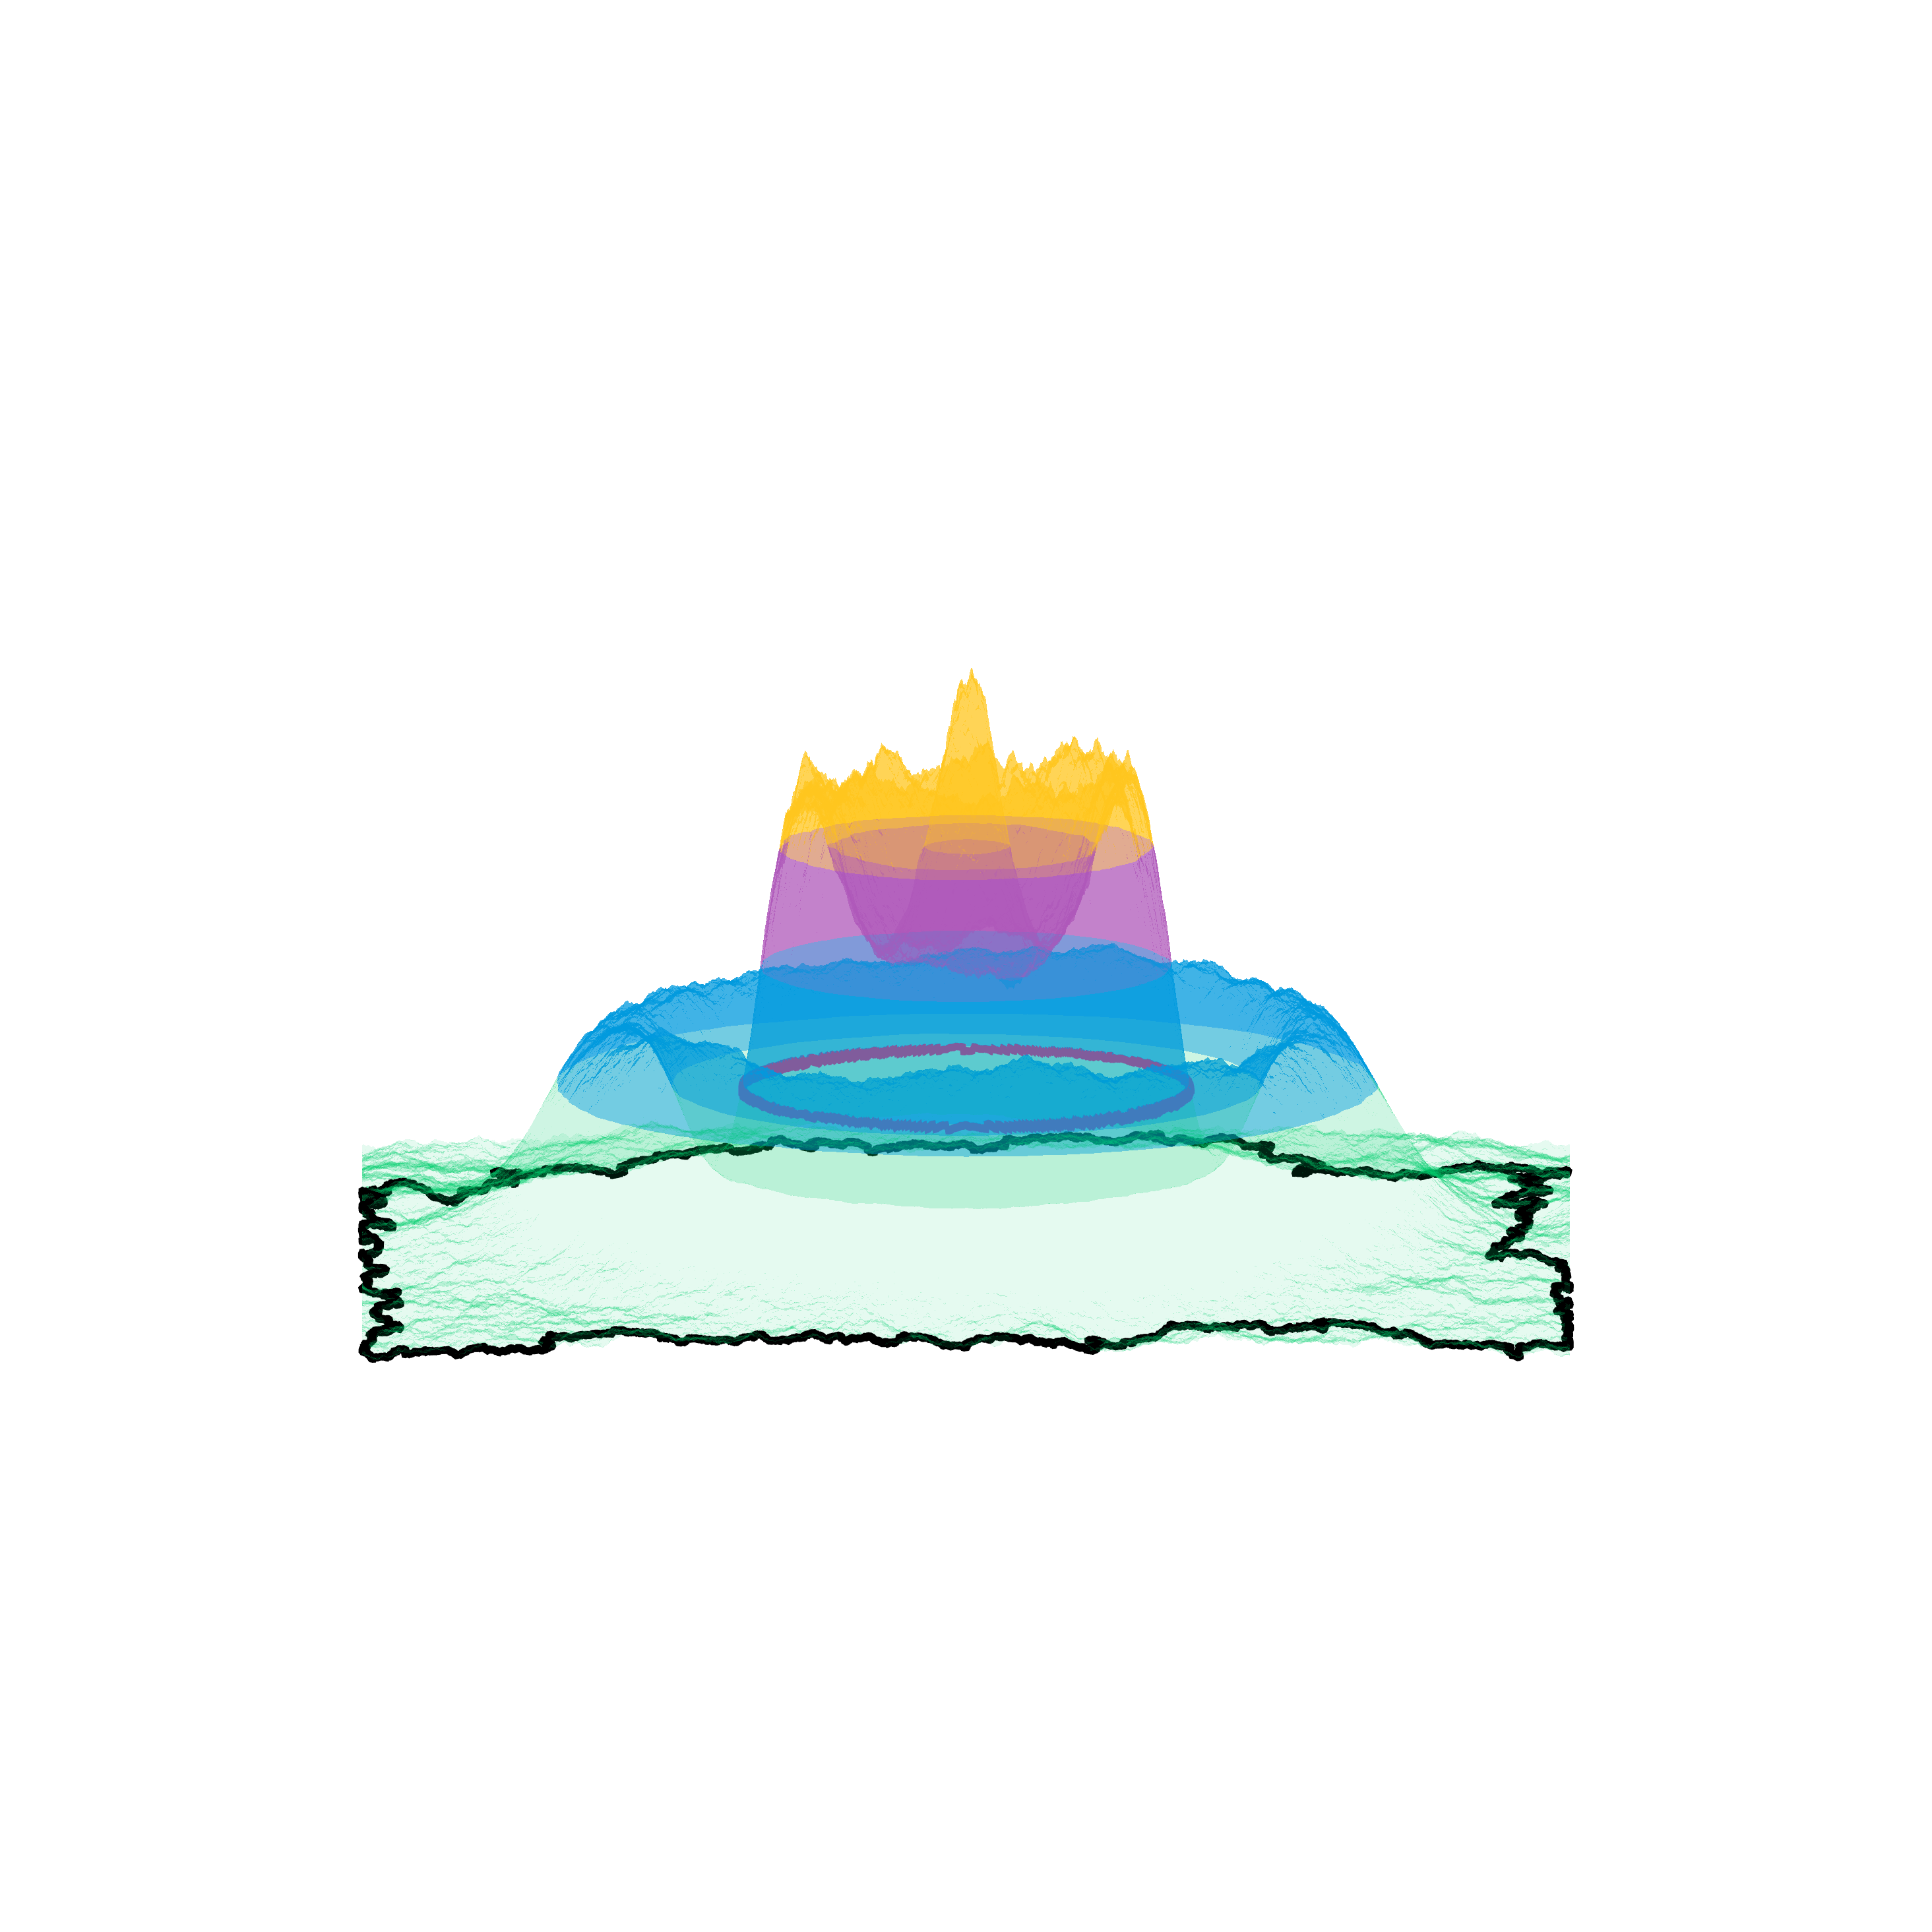
\includegraphics[trim=500 800 500 800, clip, width=0.35\textwidth]{figures/relative/surf_side-0_1.png}
  
\includegraphics[trim=500 500 500 500, clip, width=0.25\textwidth]{figures/relative/surf_top-0_1.png}
  \caption{The infinite 1-features of the restricted diagram can be matched with the infinite 2-features of the relative diagrams.
  The sequence of birth times of relative 2-features in \emph{decreasing} order correspond to the deaths of restricted 1-features in \emph{increasing} order.}\label{fig:relative2}
\end{figure}


\section{Conclusion}
% !TeX root = ../main_socg.tex

We have extended the Topological Coverage Criterion to the setting of Topological Scalar Field Analysis.
By defining the boundary in terms of a sublevel set of a scalar field we provide an interpretation of the TCC that applies more naturally to data coverage.
We then showed how the assumptions and machinery of the TCC can be used to approximate the persistent homology of the scalar field relative to a static sublevel set.
This relative persistent homology is shown to be related to a truncation of that of the scalar field as whole, and therefore provides a way to approximate a part of its persistence diagram in the presence of un-verified data.

There are a number of unanswered questions and directions for future work.
Our theoretical results were limited by our understanding of duality.
Importantly, a more rigorous treatment of duality allow us to formally link the regularity assumptions made in the TCC and our interleaving
This would allow us to merge the assumptions made in these two statements as our main theorem.
It would also simplify some of the assumptions made on our sample in the statement of the TCC.
Moreover, as duality plays a central role in the TCC it is natural to investigate its role in the analysis of scalar fields.
Our hope is to be able to provide a rigorous comparison between the relative approach and the persistent homology of the superlevel set filtration, leading to connections with Extended Persistence~\cite{cohen09extending}.
% This would not only allow us to apply duality to persistent homology~\cite{desilva11duality}, but also allow us to provide a rigorous comparison between the relative approach and the persistent homology of the superlevel set filtration and explore connections with Extended Persistence~\cite{cohen09extending}.

From a computational perspective, we are particularly interested in the matching problem discussed in Section~\ref{sec:experiments} that can be used to recover the full diagram.
Our statements in terms of sublevel sets can also be generalized to disjoint unions of sub and superlevel sets, where coverage is confirmed in an \emph{interlevel} set.
This, along with a better understanding of the duality between sub and superlevel sets could lead to an iterative approach in which the persistent homology of a scalar field is constructed as data becomes available.
% We also note that computing the diagram of a nested pair of relative Rips complexes that vary in both function values and scale is nontrivial.
% We are interested in finding efficient ways to compute these image diagrams.
% We are also interested in finding efficient ways to compute the image persistent (relative) homology that vary in both scalar and scale.

% The problem of relaxing our assumptions on the boundary can be approached from both a theoretical and computational perspective.
% Ways to avoid the isomorphism we require could be investigated in theory, and the interaction of relative persistent homology and the Persistent Nerve Lemma may be used tighten our assumptions.
% We would also like to conduct a more rigorous investigation on the effect of these assumptions in practice.


\bibliography{bibliography}

\appendix

\section{Omitted Proofs}\label{apx:omit}
% !TeX root = ../new.tex

\begin{landscape}
\begin{scriptsize}
\begin{centering}
\[\begin{tikzcd}[row sep=large, column sep=scriptsize]
  |[alias=U]| \D{\omega-c(\delta+\zeta)}{\alpha-3c\delta}
                                  \arrow[to=V, "\gamma_{\alpha-3c\delta}{[3c\delta]}"]
                                  \arrow[to=Sa, "f_{\omega-c(\delta+\zeta}{[\alpha-3c\delta]}"]
  &&&& |[alias=V]| \D{\omega}{\alpha}
                                  \arrow[to=W, "\pi_\alpha{[3c\zeta]}"]
                                  \arrow[to=Ta, "f_\omega{[\alpha]}"]
  &&&& |[alias=W]|
  \D{\omega+c(\delta+2\zeta)}{\alpha+3c\zeta}\\
  %
  & |[alias=Sa]|
  \P{\omega-c\zeta}{\delta}{\alpha-2c\delta}
                                  \arrow[to=Sb, "s_{\alpha-2c\delta}"]
                                  \arrow[to=CSa, "(\E\N_{w-c\zeta}^\delta{[\alpha-2c\delta]})^{-1}"]
  && |[alias=Sb]| \P{\omega-c\zeta}{2\delta}{\alpha-2c\delta}
                                  \arrow[to=Ta, "\vartheta_{\alpha-2c\delta}{[2c\delta+\zeta]}"]
                                  \arrow[to=V, "m_{\omega-c\zeta}^{2\delta}{[\alpha-2c\delta]}"]
  && |[alias=Ta]| \P{\omega+c\delta}{\zeta}{\alpha+c\zeta}
                                  \arrow[to=Tb, "t_{\alpha+c\zeta}"]
                                  \arrow[to=CTa, "(\E\N_{w+c\delta}^\zeta{[\alpha+c\zeta]})^{-1}"]
  && |[alias=Tb]| \P{\omega+c\delta}{2\zeta}{\alpha+c\zeta}
                                  \arrow[to=W, "m_{\omega+c\delta}^{2\zeta}{[\alpha+c\zeta]}"]
  &\\
  %
  & |[alias=CSa]|
  \CP{\omega-c\zeta}{\delta}{\alpha-2c\delta}
                                  \arrow[to=CSb, "\check{s}_{\alpha-2c\delta}"]
                                  \arrow[to=RS, "\I_{\omega-c\zeta}^\delta{[\alpha-2c\delta]}"']
  && |[alias=CSb]| \CP{\omega-c\zeta}{2\delta}{\alpha-2c\delta}
                                  \arrow[to=Sb, "\E\N_{w-c\zeta}^{2\delta}{[\alpha-2c\delta]}"]
                                  \arrow[to=CTa, "\check{\vartheta}_{\alpha-2c\delta}{[2c\delta+\zeta]}"]
  && |[alias=CTa]| \CP{\omega+c\delta}{\zeta}{\alpha+c\zeta}
                                  \arrow[to=CTb, "\check{t}_{\alpha+c\zeta}"]
                                  \arrow[to=RT, "\I_{\omega+c\delta}^\zeta{[\alpha+c\zeta]}"']
  && |[alias=CTb]| \CP{\omega+c\delta}{2\zeta}{\alpha+c\zeta}
                                  \arrow[to=Tb, "\E\N_{w+c\delta}^{2\zeta}{[\alpha+2c\zeta]}"]
  &\\
  %
  && |[alias=RS]| \CP{\omega-c\zeta}{2\delta}{\alpha-2c\delta}
                                  \arrow[to=CSb, "\J_{\omega-c\zeta}^{2\delta}{[\alpha-2c\delta]}"]
                                  \arrow[to=RT, "\rips\lambda_{\alpha-c\zeta}{[c(2\delta+\zeta)]}"]
  &&&& |[alias=RT]| \RP{\omega+c\delta}{2\zeta}{\alpha+c\zeta}
                                  \arrow[to=CTb, "\J_{\omega+c\delta}^{2\zeta}{[\alpha+c\zeta]}"]
  &&\\
\end{tikzcd}\]
\end{centering}
\end{scriptsize}
\end{landscape}


\section{Duality}\label{apx:duality}
% !TeX root = ../main.tex

For a pair $(A, B)$ in a topological space $X$ and any $R$ module $G$ let $\hom^k(A, B; G)$ denote the \textbf{singular cohomology} of $(A,B)$ (with coefficients in $G$).
Let $\hom^k_c(A, B; G)$ denote the corresponding \textbf{singular cohomology with compact support}.
For any compact pair $(A,B)$ there is an isomorphism $\hom^k_c(A, B; G)\to\hom^k(A, B; G)$.

Corollary\ref{cor:univ_coef} follows from the Universal Coefficient Theorem for singular homology (and cohomology) as vector spaces over a field $\FF$, as the dual vector space $\Hom(\hom_k(A, B), \FF)$ is isomorphic to $\hom_k(A, B; \FF)$ for any finitely generated $\hom_k(A, B)$.

\begin{corollary}\label{cor:univ_coef}
  For a topological pair $(A, B)$ and a field $\FF$ such that $\hom_k(A, B)$ is finitely generated there is a natural isomorphism
  \[\nu : \hom^k(A, B; \FF)\to \hom_k(A, B; \FF).\]
\end{corollary}

Let $\overline{\hom}^k(A, B; G)$ be the \textbf{Alexander-Spanier cohomology} of the pair $(A,B)$, defined as the limit of the direct system of neighborhoods $(U,V)$ of the pair $(A, B)$.
Let $\overline{\hom}^k_c(A, B; G)$ denote the corresponding \textbf{Alexander-Spanier cohomology with compact support} where $\overline{\hom}^k_c(A, B; G)\cong\overline{\hom}^k(A, B; G)$ for any compact pair $(A, B)$.

\begin{theorem}[\textbf{Alexander-Poincar\'e-Lefschetz Duality} (Spanier~\cite{spanier1989algebraic}, Theorem 6.2.17)]\label{thm:alexander}
  Let $X$ be an orientable $d$-manifold and $(A, B)$ be a compact pair in $X$.
  Then for all $k$ and $R$ modules $G$ there is a (natural) isomorphism
  \[\lambda : \hom_k(X\setminus B, X\setminus A; G)\to \overline{\hom}^{d-k}(A, B; G).\]
\end{theorem}

A space $X$ is said to be \textbf{homologically locally connected in dimension $n$} if for every $x\in X$ and neighborhood $U$ of $x$ there exists a neighborhood $V$ of $x$ in $U$ such that $\tilde{\hom}_n(V)\to\tilde{\hom}_n(U)$ is trivial for $k\leq n$.

\begin{lemma}[Spanier p. 341, Corollary 6.9.6]\label{lem:alexander_iso}
  Let $A$ be a closed subset, homologically locally connected in dimension $n$, of a Hausdorff space $X$, homologically locally connected in dimension $n$.
  If $X$ has the property that every open subset is paracompact, $\mu : \overline{\hom}_c^k(X,A; G)\to \hom_c^k(X, A; G)$ is an isomorphism for $k\leq n$ and a monomorphism for $q = n+1$.
\end{lemma}

In the following we will assume homology (and cohomology) over a field $\FF$.

\begin{lemma}\label{cor:alexander_iso}
  Let $X$ be an orientable $d$-manifold and $(A,B)$ a compact pair of locally path connected subspaces in $X$.
  Then
  \[\xi : \hom_d(X\setminus B, X\setminus  A)\to \hom_0(A, B)\]
  is a natural isomorphism.
\end{lemma}
\begin{proof}
  Because $X$ is orientable and $(A,B)$ are compact $\lambda : \hom_d(X\setminus B, X\setminus A)\to \overline{\hom}^{0}(A, B)$ is an isomorphism by Theorem~\ref{thm:alexander}.
  Note that
  Moreover, because every subset of $X$ is (hereditarily) paracompact every open set in $A$, with the subspace topology, is paracompact.
  For any neighborhood $U$ of a point $x$ in a locally path connected space there must exist some neighborhood $V\subset U$ of $x$ that is path connected in the subspace topology.
  As $\tilde{\hom}_0(V) = 0$ for any nonempty, path connected topological space $V$ (see Spanier p. 175, Lemma 4.4.7) it follows that $A$ (resp. $B$) are homologically locally connected in dimension $0$.
  Because $(A,B)$ is a compact pair the singular and Alexander-spanier cohomology modules of $(A,B)$ with compact support are isomorphic to those without, thus $\mu:\overline{\hom}^{0}(A, B)\to \hom^0(A, B)$ is an isomorphism.
  By Corollary~\ref{cor:univ_coef} we have a natural isomorphism $\nu : \hom^0(A, B)\to\hom_0(A, B)$ thus the composition $\xi := \nu\circ\mu\circ\lambda : \hom_d(X\setminus B, X\setminus  A)\to \hom_0(A, B)$ is a natural isomorphism.
\end{proof}

\begin{lemma}\label{lem:duality_apply}
  Let $\X$ be an orientable $d$-manifold let $D$ be a compact subset of $\X$.
  Let $P$ be a finite subset of $D$ such that $P^\e\subset \intr_\X(D)$ and $Q\subseteq P$.

  If $D\setminus Q^\e$ and $D\setminus P^\e$ are locally path connected then there is a natural isomorphism
  \[ \xi : \hom_d(P^\e,Q^\e)\to \hom_0(D\setminus Q^\e, D\setminus P^\e).\]
\end{lemma}
\begin{proof}
  Because $Q^\e$ and $P^\e$ are open in $D$ and $D$ is compact in $\X$ the complement $D\setminus Q^\e$ is closed in $D$, and therefore compact in $\X$.
  Moreover, because $P^\e\subset \intr_\X(D)$, $\hom_d(\X\setminus(D\setminus P^\e), \X\setminus(D\setminus Q^\e)) = \hom_d(P^\e, Q^\e)$.
  As we have assumed these complements are locally path connected by assumption we have a natural isomorphism $\xi : \hom_d(P^\e, Q^\e)\to \hom_0(D\setminus Q^\e, D\setminus P^\e)$
  by Lemma~\ref{cor:alexander_iso}.
  %
  % Because $\e > \varrho_D$ the covers by metric balls associated with $P^\e$ and $Q^\e$ are good, so we have isomorphisms $\N : \hom_d(\cech^\e(P, Q))\to \hom_d(P^\e, Q^\e)$ for all $Q\subseteq P$ by the Nerve Theorem.
  % So the composition $\xi\N := \xi\circ\N$ is an isomorphism.
  % Moreover, because $\xi$ is natural and $\N$ commutes with maps induced by inclusions by the persistent nerve lemma the composition $\xi\N$ does as well.
\end{proof}

% \begin{lemma}\label{lem:duality_apply}
%   Let $\X$ be an orientable $d$-manifold let $D$ be a compact subset of $\X$ with strong convexity radius $\varrho_D > \e$.
%   Let $P$ be a finite subset of $D$ such that $P^\e\subset \intr_\X(D)$ and $Q\subseteq P$.
%
%   If $D\setminus Q^\e$ and $D\setminus P^\e$ are locally path connected then there is an isomorphism
%   \[ \xi\N : \hom_d(\cech^\e(P,Q))\to \hom_0(D\setminus Q^\e, D\setminus P^\e)\]
%   that commutes with maps induced by inclusions.
% \end{lemma}
% \begin{proof}
%   Because $Q^\e$ and $P^\e$ are open in $D$ and $D$ is compact in $\X$ the complement $D\setminus Q^\e$ is closed in $D$, and therefore compact in $\X$.
%   Moreover, because $P^\e\subset \intr_\X(D)$, $\hom_d(\X\setminus(D\setminus P^\e), \X\setminus(D\setminus Q^\e)) = \hom_d(P^\e, Q^\e)$.
%   As we have assumed these complements are locally path connected by assumption we have a natural isomorphism $\xi : \hom_d(P^\e, Q^\e)\to \hom_0(D\setminus Q^\e, D\setminus P^\e)$
%   by Lemma~\ref{cor:alexander_iso}.
%
%   Because $\e > \varrho_D$ the covers by metric balls associated with $P^\e$ and $Q^\e$ are good, so we have isomorphisms $\N : \hom_d(\cech^\e(P, Q))\to \hom_d(P^\e, Q^\e)$ for all $Q\subseteq P$ by the Nerve Theorem.
%   So the composition $\xi\N := \xi\circ\N$ is an isomorphism.
%   Moreover, because $\xi$ is natural and $\N$ commutes with maps induced by inclusions by the persistent nerve lemma the composition $\xi\N$ does as well.
% \end{proof}

% The requirement that our complements are locally path connected is necessary in order to satisfy the general statement of the duality theorem.
% A rigorous investigation of the minimal assumptions that can be made on $\X$ and $D$ is beyond the scope of this paper.
% We note that, in practice, it likely suffices to assume that there exists a triangulation of $P^\e$ that is a subcomplex of some refinement of a triangulation of $\X$ (see~\cite{cavanna2017when},~\cite{julian83alexander}).


% % \begin{theorem}[\textbf{Alexander-Poincar\'e Duality} (Julian et. al.~\cite{julian83alexander}, Theorem 5.1)]\label{thm:alexander}
% %   Let $K$ be an abstract simplicial complex that is a combinatorial oriented $d$-manifold.
% %   Let $L$ be a subcomplex of some refinement of $K$ and $M$ be a subcomplex of $L$.
% %   Let $\overline{L}$ and $\overline{M}$ denote the complements of $L$ and $M$ as subcomplexes of $K$ that do not share vertices with the original complexes.
% %   Then for all $k$ there is a natural isomorphism
% %   \[ \hom^k(L, M)\to \hom_{d-k}(\overline{M},\overline{L}). \]
% % \end{theorem}
%
% % \begin{corollary}
% %   Let $X$ be a topological space and $D$ be a compact subspace of $X$.
% %   Let $(U, V)$ be a topological pair of spaces in $D$ and suppose there exists a triangulation $\Delta X$ of $X$ such that there exists triangulation $\Delta U$ of $U\subset$ that is a subcomplex of some refinement of $\Delta X$ and a triangulation $\Delta V$ of $V$ that is a subcomplex of $\Delta U$.
% %   Then for all $k$ there is a natural isomorphism
% %   \[ \hom^k(U, V)\to\hom_{d-k}(D\setminus U, D\setminus V).\]
% % \end{corollary}
%
%
% \begin{corollary}\label{cor:univ_coef}
%   Let $(A, B)$ be a topological pair and $\FF$ be a field such that $\hom_k(A, B; \FF)$ is finitely generated.
%   Then there is a natural isomorphism
%   \[\hom^k(A, B; \FF)\to \hom_k(A, B; \FF).\]
% \end{corollary}
% \begin{proof}
%   As $\mathrm{Ext}(\Hom(A, B), \FF) = 0$ for any field $\FF$ the map
%   \[\hom^k(A, B; \FF)\to \Hom(\hom_k(A, B), \FF)\]
%   in the natural short exact sequence provided by Theorem~\ref{thm:univ_coef} is a natural isomorphism.
%   The result follows from the fact that $\hom_k(A, B; \FF)$ is finitely generated, and is therefore isomorphic to the dual vector space $\Hom(\hom_k(A, B), \FF)$.
% \end{proof}
%
% % \begin{theorem}[\textbf{Universal Coefficient Theorem} (Munkres p. 337, Corollary 56.4)]\label{thm:univ_coef}
% %   Let $(A,B)$ be a topological pair such that $\hom_k(A, B)$ is finitely generated for all $k$.
% %   Then for all $k$ and any abelian group $G$ there is a natural exact sequence
% %   \[ 0\to\mathrm{Ext}(\hom^{k+1}(A, B), G)\to \hom_k(A, B; G)\to \Hom(\hom^k(A, B), G)\to 0.\]
% %   This sequence splits, but not naturally.
% % \end{theorem}
%
% \begin{theorem}
%   Let $X$ be a topological space and $D$ be a compact subspace of $X$.
%   Suppose there exists a triangulation $\Delta X$ of $X$ that is a combinatorial oriented $d$-manifold.
%   Let $(U, V)$ be a topological pair of spaces in $D$ and $\FF$ be a field such that $\hom_k(U,V;\FF)$ is finitely generated for all $k$.
%
%   If there exists a pair of triangulations $(\Delta U, \Delta V)$ of the pair $(U, V)$ such that $\Delta U$ is a subcomplex of some refinement of $\Delta X$ then there is a natural isomorphism
%   \[ \hom_d(U, V; \FF)\to \hom_0(X\setminus V, X\setminus U; \FF).\]
% \end{theorem}
% \begin{proof}
%   By Theorem~\ref{thm:alexander} we have a natural isomorphism
%   \[ \hom^d(\Delta U, \Delta V; \FF)\to \hom_{0}(\overline{\Delta V}, \overline{\Delta U}; \FF) \]
%   where $\overline{\Delta V}$ and $\overline{\Delta U}$ denote the complements of $\Delta V$ and $\Delta U$ as subcomplexes of $\Delta X$ that do not share vertices with their respective original complexes.
%   \textbf{TODO}\footnote{$\hom^d(U, V;\FF)\cong \hom^d(\Delta U, \Delta V;\FF),\ \hom_{0}(\overline{\Delta V}, \overline{\Delta U}; \FF) \cong \hom_0(X\setminus V, X\setminus U; \FF).$}
%
%   Because $\hom_d(U, V; \FF)$ is finitely generated $\hom_d(U, V;\FF)\cong\hom^d(U, V; \FF)$ by Corollary~\ref{cor:univ_coef}.
%   It follows that the composition
%   \[\hom_d(U, V; \FF)\to \hom^d(U,V;\FF)\to\hom_0(X\setminus V, X\setminus U; \FF)\]
%   is a natural isomorphism as desired.
% \end{proof}
% % \begin{proof}
% %   \begin{itemize}
% %     \item By Theorem~\ref{thm:univ_coef} we have a short exact sequence
% %       \[ 0\to\mathrm{Ext}(\hom^{d+1}(\Delta U, \Delta V), G)\to \hom_d(\Delta U, \Delta V; G)\to \Hom(\hom^d(\Delta U, \Delta V), G)\to 0\]
% %       for any abelian group $G$.
% %       Because $\Delta U,\Delta V$ are subcomplexes of the combinatorial $d$-manifold $\Delta X$, $\hom^{d+1}(\Delta U, \Delta V) = 0$, so $\hom_d(\Delta U, \Delta V; G)\to \Hom(\hom^d(\Delta U, \Delta V), G)$ is an isomorphism.
% %     \item By Theorem~\ref{thm:alexander} we have a natural isomorphism $\hom^d(\Delta U, \Delta V)\to \hom_0(\overline{\Delta V},\overline{\Delta U})$.
% %       Therefore, because we have natural\footnote{\textbf{TODO} natural short exact $\implies$ natural isomorphism.} isomorphisms $\hom_d(\Delta U, \Delta V; G)\to \Hom(\hom^d(\Delta U, \Delta V), G)$ for all abelian groups $G$, we have a natural isomorphism (\textbf{TODO} prove it).
% %       \[\hom_d(\Delta U, \Delta V)\to \hom_0(\overline{\Delta V},\overline{\Delta U}).\]
% %     \item Because $\hom_d(U, V)\cong \hom_d(\Delta U, \Delta V)$ and $\hom_0(X\setminus V, X\setminus U)\cong \hom_0(\overline{\Delta V},\overline{\Delta U})$ (\textbf{TODO} prove it\footnote{$(X\setminus V, X\setminus U)$ or $(D\setminus V, D\setminus U)$?}), we have a natural isomorphism
% %     \[ \hom_d(U, V)\to \hom_0(X\setminus V, X\setminus U). \]
% %   \end{itemize}
% % \end{proof}
%
%
% %
% % \begin{theorem}[\textbf{Alexander Duality} (Spanier p. 296, Theorem 6.2.17)]
% %   Let $U$ be an orientation over $R$ of an $d$-manifold $X$ and let $(A, B)$ be a compact pair in $X$.
% %   Then for all $k$ and $R$ modules $G$ there is a natural isomorphism
% %   \[ \hom_k(X\setminus B, X\setminus A; G)\to\overline{\hom}^{d-k}(A, B; G).\]
% % \end{theorem}
% %
% % \begin{lemma}
% %   Let $U$ be an orientation over $R$ of an $d$-manifold $X$ and let $(A, B)$ be a compact pair in $X$ such that $\hom_k(A, B)$ is finitely generated for all $k$.
% %   Then for all $R$ modules $G$ there is a natural isomorphism
% %   \[ \hom_0(X\setminus B, X\setminus A; G)\to\hom_d(A, B; G). \]
% % \end{lemma}
% % \begin{proof}
% %   \textbf{TODO}
% % \end{proof}


\end{document}
